%  ========================================================================
%  Copyright (c) 1985 The University of Washington
%
%  Licensed under the Apache License, Version 2.0 (the "License");
%  you may not use this file except in compliance with the License.
%  You may obtain a copy of the License at
%
%      http://www.apache.org/licenses/LICENSE-2.0
%
%  Unless required by applicable law or agreed to in writing, software
%  distributed under the License is distributed on an "AS IS" BASIS,
%  WITHOUT WARRANTIES OR CONDITIONS OF ANY KIND, either express or implied.
%  See the License for the specific language governing permissions and
%  limitations under the License.
%  ========================================================================
%

% Documentation for University of Washington thesis LaTeX document class
% by Jim Fox
% fox@washington.edu
%
%    Revised for version 2015/03/03 of uwthesis.cls
%    Revised, 2016/11/22, for cleanup of sample copyright and title pages
%
%    This document is contained in a single file ONLY because
%    I wanted to be able to distribute it easily.  A real thesis ought
%    to be contained on many files (e.g., one for each chapter, at least).
%
%    To help you identify the files and sections in this large file
%    I use the string '==========' to identify new files.
%
%    To help you ignore the unusual things I do with this sample document
%    I try to use the notation
%       
%    % --- sample stuff only -----
%    special stuff for my document, but you don't need it in your thesis
%    % --- end-of-sample-stuff ---


%    Printed in twoside style now that that's allowed
%
 
\documentclass [11pt, proquest, article] {uwthesis}[2016/11/22]
 
%
% The following line would print the thesis in a postscript font 

\usepackage[style=authoryear,backend=bibtex,style=numeric]{biblatex}
\def\bibpreamble{\protect\addcontentsline{toc}{chapter}{Bibliography}}
\addbibresource{uwthesis.bib}
%


\setcounter{tocdepth}{1}  % Print the chapter and sections to the toc
 

% ==========   Local defs and mods
%

% --- sample stuff only -----
% These format the sample code in this document
\usepackage{placeins}
\usepackage{amsmath}
\usepackage{fixltx2e}
\usepackage{hyperref}
\usepackage[pdftex]{graphicx}     
\usepackage{alltt}  % 
%\usepackage{hyperref}  % 
\newenvironment{demo}
  {\begin{alltt}\leftskip3em
     \def\\{\ttfamily\char`\\}%
     \def\{{\ttfamily\char`\{}%
     \def\}{\ttfamily\char`\}}}
  {\end{alltt}}
 
\hypersetup{
	colorlinks,
	citecolor=black,
	filecolor=black,
	linkcolor=black,
	urlcolor=black
}

% metafont font.  If logo not available, use the second form
%
% \font\mffont=logosl10 scaled\magstep1
\let\mffont=\sf
% --- end-of-sample-stuff ---
 



\begin{document}
 
% ==========   Preliminary pages
%
% ( revised 2012 for electronic submission )
%

%\prelimpages
 
%%
%% ----- copyright and title pages
%%
%\Title{The Suitability of the \LaTeX\ Text Formatter\\
%  for Thesis Preparation by Technical and\\
%  Non-technical Degree Candidates}
%\Author{Jim Fox}
%\Year{2016}
%\Program{IT Infrastructure}

%\Chair{Name of Chairperson}{Title of Chair}{Department of Chair}
%\Signature{First committee member}
%\Signature{Next committee member}
%\Signature{etc}
%
%\copyrightpage
%
%\titlepage  

 
%
% ----- signature and quoteslip are gone
%

%
% ----- abstract
%


%\setcounter{page}{-1}
%\abstract{%
%This sample dissertation is an aid to students who are attempting
%to format their theses with \LaTeX, a sophisticated
%text formatter widely used by mathematicians and scientists everywhere.
% 
%\begin{itemize}
%\item It describes the use of a specialized
%macro package developed specifically for thesis production
%at the University.
%The macros customize \LaTeX\ for the correct thesis style,
%allowing the student to concentrate on the substance of
%his or her text.%
%\footnote{See Appendix A to obtain the source to this
% thesis and the class file.}
%\item It demonstrates the solutions to a variety of
%formatting challenges found in thesis production.
%\item It serves as a template for a real dissertation.
%\end{itemize}
%}
 
%
% ----- contents & etc.
%
\tableofcontents
\raggedbottom
%\listoffigures
%%\listoftables  % I have no tables
% 
%%
%% ----- glossary 
%%
%\chapter*{Glossary}      % starred form omits the `chapter x'
%\addcontentsline{toc}{chapter}{Glossary}
%\thispagestyle{plain}
%%
%\begin{glossary}
%\item[argument] replacement text which customizes a \LaTeX\ macro for
%each particular usage.
%\item[back-up] a copy of a file to be used when catastrophe strikes
%the original.  People who make no back-ups deserve
%no sympathy.
%\item[control sequence] the normal form of a command to \LaTeX.
%\item[delimiter] something, often a character, that indicates
%the beginning and ending of an argument.
%More generally, a delimiter is a field separator.
%\item[document class] a file of macros that tailors \LaTeX\ for
%a particular document.  The macros described by this thesis
%constitute a document class.
%\item[document option] a macro or file of macros
%that further modifies \LaTeX\ for
%a particular document.  The option {\tt[chapternotes]}
%constitutes a document option.
%\item[figure] illustrated material, including graphs,
%diagrams, drawings and photographs.
%\item[font] a character set (the alphabet plus digits
%and special symbols) of a particular size and style.  A couple of fonts
%used in this thesis are twelve point roman and {\sl twelve point roman
%slanted}.
%\item[footnote] a note placed at the bottom of a page, end of a chapter,
%or end of a thesis that comments on or cites a reference
%for a designated part of the text.
%\item[formatter] (as opposed to a word-processor) arranges printed
%material according to instructions embedded in the text.
%A word-processor, on the other hand, is normally controlled
%by keyboard strokes that move text about on a display.
%\item[\LaTeX] simply the ultimate in computerized typesetting.
%\item[macro]  a complex control sequence composed of 
%other control sequences.
%\item[pica] an archaic unit of length.  One pica is twelve points and
%six picas is about an inch.
%\item[point] a unit of length.  72.27 points equals one inch.
%\item[roman]  a conventional printing typestyle using serifs.
%the decorations on the ends of letter strokes.
%This thesis is set in roman type.
%\item[rule] a straight printed line; e.g., \hrulefill.
%\item[serif] the decoration at the ends of letter strokes.
%\item[table] information placed in a columnar arrangement.
%\item[thesis] either a master's thesis or a doctoral dissertation.
%This document also refers to itself as a thesis, although it
%really is not one.
% 
%\end{glossary}
% 
%%
%% ----- acknowledgments
%%
%\acknowledgments{% \vskip2pc
%  % {\narrower\noindent
%  The author wishes to express sincere appreciation to
%  University of Washington, where he has had the opportunity
%  to work with the \TeX\ formatting system,
%  and to the author of \TeX, Donald Knuth, {\it il miglior fabbro}.
%  % \par}
%}

%
% ----- dedication
%
%\dedication{\begin{center}to my dear wife, Joanna\end{center}}

%
% end of the preliminary pages
 
 
 
%
% ==========      Text pages
%

\textpages
 
% ========== Chapter 1
 
\chapter {Introduction}
 
In this thesis I introduce the development of new techniques for the production of materials in the warm dense matter (WDM) regime, and for interrogation of the structure and thermodynamic state of such systems using x-ray diffraction and (to a lesser extent) spectroscopy. The main results include a scheme for single-shot determination of the static structure factors of WDM systems generated at laser plasma facilities; a technique for enhancing the density of deposited energy in WDM generated at fourth-generation X-ray sources such as the Linac Coherent Light Source (LCLS); and interpretation of experimental data that puts new constraints on the thermalization (both electronic and lattice) of a solid state material upon fs-scale XFEL heating. In addition to this thread of research I discuss some secondary work on the development of software and electronics for energy- and position-sensitive pixel detectors including current applications in the context of soft x-ray laboratory and possible future ones in XFEL, synchrotron, and laser plasma facility-based experiments.

\begin{figure}[h] 
\caption{The atlas of high-energy density physics (cite)}
\label{fig:atlas}
\centering
\includegraphics[scale=0.25]{../Figures/atlas.png}
\end{figure}

Before proceeding it is useful to define WDM in terms of the microphysical context it occupies. Fig. \ref{fig:atlas} presents a map of thermodynamic parameter space, with the logarithm of density and temperature on the horizontal and vertical axes, respectively. A few bounding curves can be identified. First, ionization occurs at temperatures exceeding approximately 1 eV; this is denoted by curve (a), which forms a boundary between the plasma and condensed matter regimes. Second, curve (b) indicates the boundary at which the Fermi energy is approximately equal to the average thermal energy $k_BT$; i.e. where the electron degeneracy parameter, $E_f/k_B T$ is of order unity. Third, curve (c) corresponds to a value of 1 for the ratio of the Coulomb energy to the thermal to the thermal one, also called the plasma coupling parameter  $\Gamma$. 

Above curves (a), (b) and (c) is the regime of classical plasma physics where, as a result of the weak interaction between neighboring ions ($\Gamma << 1$), collective interactions predominate over binary collisions and quantum statistics can be neglected ($\Lambda << 1$) except for the purpose of calculating blackbody spectra. In this regime continuous, classical modeling treatments are widely-used and fully validated (cites). Below curves (a), (b), and (c) is the low-temperature, intermediate-density realm of condensed matter physics, where the established theoretical framework is that of many-body quantum mechanics, wherein the potential landscape is built on the interaction between electrons and ion cores. In this framework finite-temperature effects are incorporated perturbatively. WDM occupies the transitional regime above curve (a) and near the intersection of curves (b) and (c), characterized by partial degeneracy and strong ion-ion coupling ($\Gamma$ and $\Lambda$ of order unity). As a result, treatments of plasma physics originating in the classical regime are not applicable to WDM. Solid state physics models similarly fail in the WDM regime due to large, non-perturbative effects of finite temperature on the structure and thermodynamics of WDM (cites).  

Modeling of the ionization potential depression (IPD) in a plasma is a case in point of the difficulties that manifest themselves with theoretical treatments of WDM. Adequate descriptions of IPD are given the Debye-Hueckel approximation and ion sphere model, which cover opposite regimes of high temperature and low density, and low density and high temperature, respectively. We here briefly introduce both models, with focus on the assumptions and approximations that they adopt.

The Debye-Hueckel model applies to a weakly-coupled plasma in local thermal equilibrium. It identifies the electrostatic potential in the Poisson equation with the mean field generated by a population of Maxwell-Boltzmann-distributed ions or electrolytes. This results in the Poisson-Boltzmann equation which, when solved, gives the electrostatic potential produced by an arbitrary charge distribution. The condition for validity of the Debye-Hueckel model is for the Thomas-Fermi screening length (also called the Debye length) to be much larger than the mean inter-ion separation. This condition is satisfied at comparable temperatures, but lower densities, than those encompassed by the WDM regime. (check that this is right, and cite)
%Debye-Hueckel validity: cite 
%Electronic energy-levels in dense plasmas
%Richard M More
%Journal of quantitative spectroscopy & radiative transfer , 1982, Vol.27(3), p.345-357
% Need cites showing experimental validity of DH model

In the opposite limit, the ion-sphere model describes IPD in a high-density material with $\Gamma > 1$ (in the low-temperature context IPD is more commonly referred to as pressure ionization). The picture offered by the ion-sphere model is that of a plasma with highly-correlated ion positions and therefore no close encounters between ion pairs. Each ion is treated as a sphere whose potential is unaffected by the presence of neighboring ions. (cite Stewart-Pyatt). The sphere radius is $R_0 = (3/4 \pi N_i)^{1/3}$, where $N_i$ is ion number density, while the orbital radius of the ion sphere's $n$th principal energy level is approximately $r_n = (n^2/Z_n)(0.529 \AA$. For the $n$th bound state to exist it is necessary that $r_n \leq R_0$; thus, IPD manifests itself as a reduction in the number of bound states as a function of the inter-ion distance $R_0$. It should be noted that, although the ion-sphere model is a frequently-used heuristic in high-temperature plasmas with near-ambient densities, it is known to be incorrect in the high-density, strongly-coupled ($\Gamma >> 1$) regime. Neaton et al. have done ab-initio (DFT) simulation of Li--a free electron-like material under ambient conditions--showing that, contrary to intuitive expectations and the ion-sphere model, it becomes less free-electron like at high densities and additionally loses its common bcc crystal structure. (cite Neaton 1999) Due to overlap of core electrons, the distortion of electronic wavefunctions in this regime is strongly nonperturbative--again in conflict with the ion-sphere model's assumptions. 



% TODO: need stuff here on the validity of the ion sphere model
% Cite Zimmerman and More 1979

Leaving aside, momentarily, the ion sphere model's limitations, we might contemplate constructing a model of ionization potential depression that reduces to the ion sphere and Debye-Hueckel models in their respective limits. Doing so is challenging because it allows none of the simplifying approximations invoked by the two limiting cases. One manifestation of the lack of consensus concerning the correct approach is the existence of two mutually-contradictory models for IPD in WDM, those of Stewart and Pyatt (cite) and Ecker and Kroll (cite). Though the Stewart-Pyatt model is more widely used and has the virtue of reproducing the ion-sphere and Debye-Hueckel behaviors (cite Crowley review article), its validity has been called into question by recent direct XFEL-measurements of IPD in Al heated to 180 eV (cite Ciricosta paper). Such conflicts exemplify the persistent difficulty of constructing models with validity across different sub-regimes of WDM.
% TODO: insert Fig. 2 from Ciricosta paper.
% TODO: talk about XRTS data interpretation issues


\section{Motivations for study of WDM}
In addition to the basic physics questions intrinsic to the WDM regime, there are a number of points of contact between WDM and particular problems in other fields. This interaction has been bolstered in recent years by rapid development of laser plasma facilities and x-ray free electron lasers (XFELs) with unprecedented experimental capability for producing WDM and probing its physical properties. This has brought many previously-intractable physical regimes into the scope of both empirical investigation and numerical simulation.  

\subsection{Astrophysical modeling}
A large contribution to this growth in interest is the relevance of WDM theory as a microphysical basis on for models of various systems in planetary and stellar astrophysics. Here we introduce two examples in which this relationship is salient.

The interiors of both rocky and gas giant planets contain dense, and in some cases Fermi-degenerate, plasmas at 1 eV-scale temperatures. Examples include the iron under conditions of the earth's core (pressure = 3 Mbar; T = 6000 K), whose viscosity and equation of state (EOS) has consequences on convective heat transfer and the formation of earth's magnetic field. (cites) Similarly, modeling of the evolution and structure of gas giant planets depends on the EOS of H under the regime of gas giant interiors. The existence of metallic H caused by pressure ionization at Mbar-scale pressures has been experimentally demonstrated, but its onset is poorly understood at the level of theoretical models for the EOS: although a first-order dielectric-to-metal phase transition has been postulated, current approaches do not attempt to model pressure ionization, instead limiting themselves to interpolation between the better-understood atomic and fully ionized limits. (cites)

% TODO Probably need more of a transition here, talk about the consequences of uncertainty in the behavior
% of metallic H
The solubility physics of binary WDM mixtures combining H with species found in rocky planetary bodies has direct consequences on mass transport across the core-mantle boundary in gas giant planets. It also has crucial importance in the modeling of gas giant formation, where the solubility of H with rocky elements bears on the plausibility of the planetesimal accretion hypothesis for gas giant genesis, which requires condensation of H and He around a rocky core. (cite Wilson MgO solubility paper). 

\begin{figure}[h] 
\caption{Saturation solubility of MgO in H as a function of pressure and temperature from \emph{ab initio} calculation by Wilson et al. The temperature conditions of the core-mantle boundaries of Saturn and Jupiter are indicated. (cite Wilson)}
\label{fig:wilson}
\centering
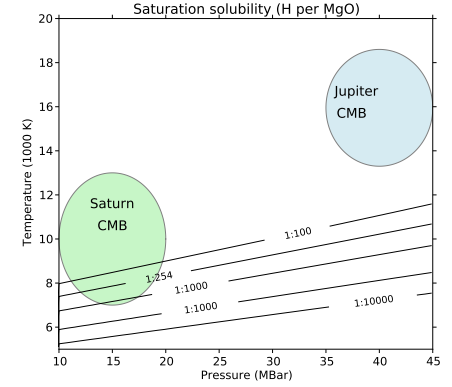
\includegraphics[scale=0.65]{../Figures/wilson_solubility.png}
\end{figure}

% cite doi:10.1088/1742-6596/717/1/012082 (Sterne et al., equations of state for ablator materials in inertial confinement fusion simulations) on the pressure ionization stuff
% cite Weir et al., Metallization of Fluid Molecular Hydrogen at 140 GPa
% cite Ebeling and Richert, PLASMA PHASE TRANSITION IN HYDROGEN 
%(cite koenig et al, doi: http://dx.doi.org/10.1088/0741-3335/47/12B/S31)
% other questions: is convection possible in the metallic H core, etc., see pg 91 of x-games

Another case in which the material properties of warm dense matter determine the behavior of an astrophysical object is that of white dwarfs, whose envelopes consist of a hot, partially Fermi-degenerate plasma. Modeling the cooling of white dwarfs is a topic of interest (cites), especially in the context of the importance of type 1a supernovae as `standard candles' for measuring distances to distant galaxies. Doing so, however, requires knowledge of stellar envelope opacities, equations of state (EOS), and transport properties, many of which properties are currently unknown to within factors of order unity. The absence of understanding of the simplest available system--the hydrogenic one-component plasma--underscores the difficulty of this thread of research.
% cites needed, see pg 58 of x-games

\subsection{Inertial Confinement Fusion}
The effort to reach controlled fusion through implosion of deuterium-tritium fuel capsules--an approach termed inertial confinement fusion--has progressed significantly in the last decade due to completion of laboratory facilities capable of producing high-energy density (HED) plasmas with densities and temperatures approaching levels needed for ignition. Fig. \ref{icf} shows a schematic of an ignition technique called indirect drive. In this configuration the ICF target, which consists of a hollow spherical capsule of ablator material filled with deuterium-tritium fuel, is confined in a hollow capsule of a high-Z material (the Hohlraum). A multi-TW, ns-duration duration laser passes through apertures in the Hohlraum and heats the Hohlraum to blackbody temperatures on the order of several hundred eV. The resulting thermal spectrum of soft X rays isotropically heats and ablates the fuel capsule's surface, causing its interior to implode by conservation of momentum. Typical parameters of the plasma created at maximum compression include areal densities (capsule density x radius) of 0.3 g/cm$^2$ and temperatures of the order 10 keV. (cites)%. see x-games pg 113)

\begin{figure}[h] 
\caption{Schematic of indirect-drive inertial confinement fusion shot. (cite)}
\label{icf}
%(cite https://lasers.llnl.gov/science/icf/how-icf-works)}
\centering
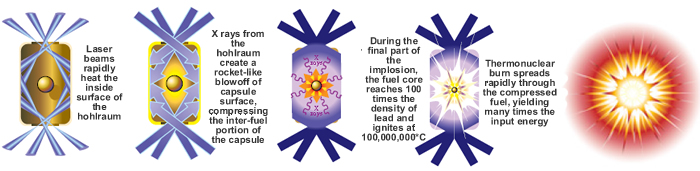
\includegraphics[scale=0.5]{../Figures/indirect-drive.jpg}
\end{figure}

Although its end state falls well within the regime of a classical plasma, the fuel capsule transitions through the WDM state during compression. The opacity and EOS of warm dense matter therefore has a strong influence on the development and propagation of shocks during ablation of the fuel capsule, which in turn affects the optimization of various experimental parameters, including fuel capsule geometry and temporal profile of the laser driver. Accurate modeling of the fuel capsule's transport properties under the WDM regime is equally important for understanding the development during compression of hydrodynamic instabilities, which are known to be a major obstacle to the efficient coupling of laser energy into fuel compression (cites).
% cite doi:10.1088/1742-6596/717/1/012082 (Sterne et al., equations of state for ablator materials in inertial confinement fusion simulations)
%TODO: cite D A Callahan, D E Hinkel, R L Berger on NIF Hohlraum temperature
% don't necessarily cite, but saumon et al. 1995 is a good reference on EOS modeling approaches.
% TODO: can say more about ICF if extra length is needed

\section{Experimental Generation of WDM}
WDM conditions may be generated using X-ray free electron lasers (XFELs) and several varieties of lasers, found both in large-scale facilities and laboratory-scale systems. Here we provide an overview of existing technologies. 
\subsection{Long-pulse lasers}
% TODO: how rapidly does the coronal plasma form?
%(TODO: equation for laser wavelength critical density
Lasers with pulse durations on the order of nanoseconds and energies of 1 kJ or more are among the most versatile tools for producing high energy density states, including warm dense matter. In the most common use cases of long pulse lasers the target is a bulk material, and coupling of laser energy into it occurs in two stages. First, the laser rapidly  generates a coronal plasma at the material's surface. Once the electron density of this plasma exceeds the laser wavelength's critical density  the laser becomes electromagnetically shielded from the material's interior and can no longer transfer energy to it. In the context of direct drive (where the material is a target to which laser energy is directly coupled), subsequent energy transfer occurs by thermal conduction of energy from the surface plasma to higher-density regions as well as by compression of the target resulting from ablation of its surface. In the case of indirect drive, the laser's energy is used to heat a surface (typically the interior of a Hohlraum) that provides a thermal bath which, in turn, couples to the target via its blackbody radiation. 

The ns duration of long-pulse lasers matches the timescale on which mechanical and hydrodynamic processes occur on typical target scales. Long-pulse lasers are thus suited to generating ramp and shock compression, notably including for the application of ICF. The largest-scale laser plasma facilities--Omega EP at the Laboratory for Laser Energetics in Rochester, NY and the National Ignition Facility--are long-pulse laser systems targeted toward the ICF program.

% TODO: pull stuff on tie-in with ICF from Brian's thesis

\subsection{Short-pulse lasers}
Short pulse lasers are a second class of systems used to generate HED conditions. They are typically defined by pulse durations on the order of a picosecond or less, down to as little as $\sim$1 fs. 

% TODO: what applications do short pulse lasers excel at?
Short-pulse laser systems arose after the development of chirped pulse amplification in the 1980s (cite) and have proliferated ever since (cites), especially with the recent advent of compact (university laboratory-scale) versions with tens of Joules of pulse energy, sufficient to generate scientifically interesting HED conditions. The largest-scale short pulse lasers have pulse powers up to 100 TW, with durations on the order of 10 to 100 fs.

Due to the smaller total energies of short-pulse lasers and the relatively slow cooling timescale of materials heated above ambient conditions \textit{regardless} of the pump duration, short-pulse lasers are used to generate HED conditions under direct-drive configurations alone. Energy is coupled into a target indirectly (as is the case with long-pulse systems) via `hot' MeV-scale electrons generated in the laser's interaction with plasma at the target surface. In the (typical) case where bulk heating is required, the target thickness is small compared to the hot electrons' stopping range, causing them to reflux through the target once it acquires net positive charge. This process lasts on the order of one ps (cite Nilson) and thus sets the time resolution of experiments in which the short-pulse laser is used to both heat and probe the target.

\label{foobar}
\subsection{X-Ray Free Electron Lasers}
The advent of X-Ray Free Electron lasers is a major advance in capability for WDM research. Existing incarnations of these sources, notably the Linac Coherent Light Source (LCLS), provide $10^{14}$ photons in a $\geq 10$ fs-duration monochromatic pulses with tunable energy. While the energies per pulse are smaller than those attainable with a short-pulse laser, they are largely sufficient to produce HED states with temperatures in excess of 100 eV (cite). Because XFELs can heat volumetrically, they are free of the primary deficiency of lasers with respect to the task of generating dense plasmas: namely, the latter can only heat bulk materials indirectly and over durations of 1 ps or longer, which exceeds the timescale for changes in WDM, preventing the study of short-lived transient states.

The ability to generate (and probe) WDM on truly inertial timescales, wherein atomic nuclei are effectively frozen, has been duly exploited in early pioneering studies at the LCLS. It forms the basis, for example, for a new thread of materials science research on nonthermal lattice and spin dynamics (cite Lee and others). Likely even more significantly, it is the enabling feature for macromolecular crystallography under the `diffract before destroy' paradigm. (cites) The possibilities surrounding rapid generation of WDM is a topic to which I return in chapters \ref{hef} and \ref{mgo}. (cite Vinko et al. and other early LCLS papers).

% TODO: insert figure Brightness_overview.jpg and cite doi:10.1038/nphoton.2007.76
% cite Richard W. Lee, Stephen J. Moon, and Hyun-Kyung Chung 2003
% cite Lee Non-thermal dynamics of the spin and charge order in striped nickelates

\section{X-ray diagnostics of WDM}
Experimental studies of WDM suffer from a substantial complication: the opacity of WDM to photons is large at energies up to the soft X ray regime. As mentioned in section \ref{foobar}, in the context of laser heating this is merely a frustration; for the purposes of measuring the conditions of a bulk WDM system, however, the need for direct detection of radiation originating from the target's interior makes optical probes wholly ineffective. Determination of the structure and thermodynamic state variables of a dense plasma therefore requires sufficiently penetrating radiation; for this reason, the large majority of WDM diagnostics are X ray photon-in photon-out measurements. 

In the remainder of this section I provide an overview of the various available techniques.
% TODo: more text...
% TODO: plot of opacity vs T and rho, or somehting like that

\subsection{Scattering}
Elastic scattering and nonresonant inelastic X-ray scattering (NIXS) are among the most-frequently probed signals for inferring the structure, temperature and ionization state of WDM. In dense plasmas generated by long-pulse lasers, where LTE is commonly assumed, NIXS also serves as a probe of temperature.

For a given sample, the sum of scattering interactions is characterized by the double-differential scattering cross section (DDCS) $d^2\sigma/d\Omega d\omega$, which describes the probability of a photon to scatter into a solid angle increment $d\Omega$ within an energy loss interval $d\omega$. Within the independent-electron and first Born approximations the DDCS is given by

\begin{equation} \label{ddcs}
\frac{d^2\sigma}{d\Omega d\omega} = r_0^2 (\frac{\omega_2}{\omega_1}) |\epsilon_1 \times \epsilon_2^*|^2 S(\vec{q}, \omega),
\end{equation}

where 


\begin{equation} \label{sofq}
S(\vec{q}, \omega) \equiv \sum_F  \sum_j\langle F|  exp(i \vec{q} \cdot \vec{r}_j) |I\rangle |^2 \delta(E_F - E_I - \hbar \omega).
\end{equation}

The first term in equation \ref{ddcs} is the Thomson cross section, which describes the interaction between a probe photon and a single electron; $S(\vec{q}, \omega)$ is referred to as the dynamic structure factor, and encapsulates all system-specific properties. $I$ and $F$ are initial and final states of the sample with energies $E_I$ and $E_F$, respectively, and the second summation in \ref{sofq} is over electrons in the scatterer.

Following Chihara (cite Chihara), the typical treatment of a dense plasma separates the dynamic structure factor into several components:

\begin{equation}
S(\vec{q}, \omega) = |f_I(q) + f_e(q)|^2 S_{ii}(q, \omega) + S_{ff}(q, \omega) + S_{bf}(q, \omega),
\end{equation}

$S_{ii}$ is the atomic/ionic structure factor, $f_I$ and $f_e$ are the form factors for the ion and a surrounding cloud of screening charge. $S_{ff}$ contains scattering from free, delocalized electrons, and $S_{bf}$ represents Raman-type bound-free transitions resulting from scattering from tightly-bound core level electrons. Note that spherical symmetry has been assumed: all terms of the structure factor depend only on the magnitude of $\vec{q}$.

The first term corresponds to elastic ($\omega = 0$) scattering, and is connected to the dense plasma's pair distribution function by a Fourier transform. Though not a component of the NIXS signal, it must often be considered in simulations and analyses of NIXS data, wherein the Bethe sum rule (cite) and other conserved quantities consist of integrals over the entire energy-loss domain of the dynamic structure factor. Elastic scattering is a highly-useful probe of structure; we consider it separately in section \ref{coh}. 

The free-free contribution to $S(q, \omega)$ can be expressed in terms of the free-electron dielectric function $\epsilon(q, \omega)$  via the fluctuation-dissipation theorem (cite Kubo et al.):

\begin{equation}
S(q, \omega) = \frac{\epsilon_0 \hbar q^2}{\pi e^2 n_e} \frac{1}{1 - e^{\hbar \omega/k_B T_e}} \Im\frac{1}{\epsilon(q, \omega)},
\end{equation}

The random phase approximation (RPA) (cite Bohm and Pines) is typically used as an approximation for $\epsilon(q, \omega)$, but more recent treatments incorporate a perturbative treatment of electron-ion interactions using the Born-Mermin Approximation (cite Mermin). 
The scattering contribution of $S_{ff}$ consists of a pair of plasmon peaks with opposite, equal-magnitude energy offsets from the elastic scattering peak. Electron density is inferred from the magnitude of the Plasmon peak shifts while temperature is obtained from the ratio of intensities of the two peaks, following the principle of detailed balance (cite Glenzer 2007 and Lee 2009).
% TODO: find and add that figure (see below)
% As shown in Fig. (which figure?), the scattering contribution of $S_{ff}$ consists of a pair of Plasmon peaks with opposite, equal-magnitude energy offsets from the elastic scattering peak. Electron density is inferred from the magnitude of the Plasmon peak shifts while temperature is obtained from the ratio of intensities of the two peaks, following the principle of detailed balance (cite Glenzer 2007 and Lee 2009).
% R Kubo.  The fluctuation-dissipation theorem.  Reports on Progress in Physics, 29(1):255, 1966.
% David Bohm and David Pines. A collective description of electron interactions: Iii.  coulomb interactions in a degenerate electron gas. Phys. Rev., 92:609–625, Nov 1953.
%N. D. Mermin. Lindhard dielectric function in the relaxation-time approximation.  Phys. Rev. B, 1:2362–2363, Mar 1970.
% figure comes from Lee 2009

Although the connection of temperature and density to the free-free component of the dielectric function is well-founded, there are two obstacles to effective interpretation of collective scattering data from WDM systems; one is theoretical and the other experimental. First, the validity of established treatments of the dielectric function has been called into question, with recent plasmon spectrum calculations based on MD-DFT simulations showing a significant change in the plasmon profile compared to that predicted by the Born-Mermin Approximation. (cite Mattern thesis and Plagemann). Second, the plasmon peak suffers from poor signal to background and has a small separation from the elastic scattering peak under typical WDM electron densities, making it difficult to resolve. As a result only a handful of experiments to date have pursued this technique. 

We finally turn our attention to the last term of \ref{sofq}, $S_{bf}$, whose contribution to the inelastic DDCS is often referred to as x-ray Thomson scattering (XRTS). Obtaining state variable information from a system's bound-free scattering contribution is dependent on the underlying model of electronic structure used; as a result, various treatments exist, including the Impulse Approximation (IA) of Eisenberger and Platzman, wherein the bound-free contribution to XRTS is equivalent to Doppler-broadened Compton scattering (cite Eisenberger and Platzman); the plane wave form factor approximation (PWFFA) of Schumacher (cite Schumacher), which attempts to extend the IA by incorporating electron binding energies; and calculation of matrix elements using a real space Green's function (RSGF) formalism applied to atomic clusters, as implemented in the atomic spectroscopy code FEFF (cite Mattern).

% TODO: need to track down the paper...
%\begin{figure}[h] \label{fig:lee}
%\caption{}
%\centering
%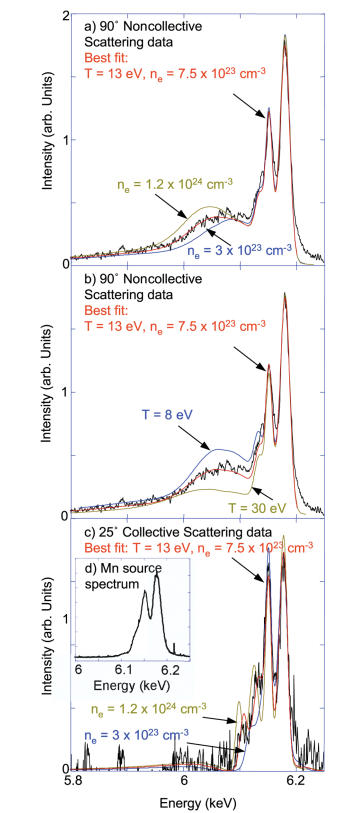
\includegraphics[scale=0.5]{../Figures/lee_xrts.png}
%\end{figure}

% TODO: examples of fruitful outcomes of WDM XRTS
% TODO: (do predicitons of XRTS heavily depend on the choice of model, or is it just that uncertainties are high, regardless of the choice?) check brian's work
In current practice, measurement of the  bound-free component of XRTS from WDM is performed in the large-$q$ regime, where the Compton feature is broad and can be measured using high-efficiency (but low-resolution) HOPG-based spectrometers (need cites for this). As such, single-particle bound-free scattering is more readily measured than collective excitation features. Since an early demonstration of the technique by Glenzer et al. (cite Glenzer 2003) it has been frequently implemented at both laser plasma and XFEL facilities (cite figures showing how these experiments are set up). Despite some fruitful outcomes, the large statistical uncertainties in XRTS spectra--particularly at laser plasma facilities, where single-shot measurements are photon-starved--make the inference of state variables difficult, and dependent on one's choice of electronic structure model. \cite{mattern2013condensed} Mattern et al. have demonstrated this concretely by comparing theoretical fits to XRTS data of shock-compressed Be, and argue that the lack of rigorous validation of electronic structure models for WDM models strongly undermines their validity for first-principles measurement of state variables. 
%With this context as motivation, we revisit the topic of WDM thermometry in chapter (reference chapter).
% S. H. Glenzer, G. Gregori, F. J. Rogers, D. H. Froula, S. W. Pollaine, R. S. Wallace, and O. L. Landen. X-ray scattering from solid density plasmas. Physics of Plasmas, 10(6):2433–2441, 2003.
% TODO fix the terminology here. Does XRTS refer to just bound-free contribution (don't think so)

\label{coh}
\subsection{Coherent Scattering}
Coherent scattering is the zero-energy loss component of the double differential cross section.  The inference of structural information from coherent scattering varies by material; two primary cases present themselves.

%, consisting of the contribution of terms in equation \ref{sofq} with  $\langle I| = \langle F|$. From equation \ref{sofq} ts differential cross section $d\sigma_{coh}/d\Omega$ has the simple proportionality
%
%\begin{equation}
%\frac{d\sigma_{coh}}{d\Omega} \propto \Sigma_j exp(i \vec{q} \cdot \vec{r}_j) 
%\end{equation}
%finish this..............


First, for amorphous materials, such as hot dense plasmas generated by ramp- or shock-compression and lacking long-range order, the scattering amplitude is isotropic and is characterized by the one-dimensional static structure factor, which is connected by a Fourier transform to the material's pair correlation function. Inference of the full pair correlation function is in practice frustrated by the difficulty of inverting a limited momentum transfer range-sampling of the structure factor, but even in the most information-limited scenarios a density can nevertheless be recovered from the structure factor's first correlation peak. Although coherent scattering measurements from dense plasmas have been demonstrated in the context of long-pulse laser compression experiments, implementation difficulties unique to that environment prevent its adoption as a routine technique. We address these difficulties, and proposed solutions, in chapter \ref{hef}. (cite Ma et al).

Second, in materials with long-range crystalline order, as typically found in XFEL-based experiments (whose timescales are shorter than the thermalization rate of electronic and ionic degrees of freedom), the coherent scattering amplitude is given by

\begin{equation}
F(\vec{q}) = \sum e^{i \vec{q} \cdot \vec{R_n}} \sum f_j(\vec{q}) e^{i \vec{q} \cdot \vec{r_j}},
\end{equation}

where the first summation is over all lattice vectors $\vec{R_n}$ and the second, referred to as the \emph{unit cell structure factor}, is over positions $\vec{r_j}$ of atoms within the unit cell. By the convolution theorem, the crystal's scattering amplitude in reciprocal space is equal to the product of the lattice and unit cell structure factor. The coherent scattering signal is therefore a discrete sampling of the unit cell structure factor at individual Bragg peaks with momentum transfers corresponding to vectors of the reciprocal lattice.

\begin{figure}[h] 
\caption{Experimental elastic scattering intensity of shock-compressed Al at OMEGA-60, compared to several hypernetted chain (HNC), Debye-Hueckel (DH), and screened one-component plasma (SOCP) models. (cite Ma et al.)}
\label{fig:ma}
%(cite https://lasers.llnl.gov/science/icf/how-icf-works)}
\centering
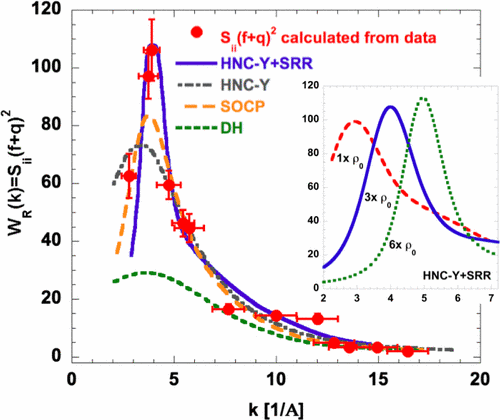
\includegraphics[scale=0.5]{../Figures/ma_Al.png}
\end{figure}

In the context of XRD from a material undergoing thermalization under fs XFEL heating, the crystal scattering amplitude's decomposition into lattice and unit cell components has a direct correspondence to interpretation of structural change. The onset of long-range lattice disorder is readily identifiable as a quenching in Bragg peaks roughly proportional to $e^{-q^2}$. Evolution of the unit cell structure factor, on the other hand, is dependent on the details of atomic level populations and the material's finite-temperature electronic structure, and can be used as a test of competing theoretical models of both. 

(need cites and discussion of the existing literature on XRD of XFEL-heated WDM)




\subsection{X-ray absorption}
X-ray absorption spectroscopy (XAS) may be used to measure the structure and unoccupied electronic density of states of WDM systems. The information available by X-ray absorption near-edge spectroscopy (XANES) and X-ray absorption fine structure (XAFS) is the same as in other scientific contexts, but the experimental implementation differs in a few respects. In all instances, the short duration of WDM states requires instantaneous collection of absorption spectra using a source with broad-band spectrum. At laser plasma facilities this is arranged using a spherical capsule of CH polymer imploded using a long-pulse laser (cite Yaakobi 2003) that emits a thermal spectrum with a \textbackslash 1 MeV temperature (check this). This so-called broadband backlighter has been used to collect XAFS for the study of compression-induced phase transitions, such as that from bcc to hcp Fe driven by ns shock-compression (cite Yaakobi 2005).

\begin{figure}[h] 
\caption{FEFF calculation of XAFS for hcp and bcc phases of Fe (a), compared to experimental data taken on ambient and shock-compressed Fe at the OMEGA laser (b). (cite Yaakobi)}
\label{fig:xafs}
%(cite https://lasers.llnl.gov/science/icf/how-icf-works)}
\centering
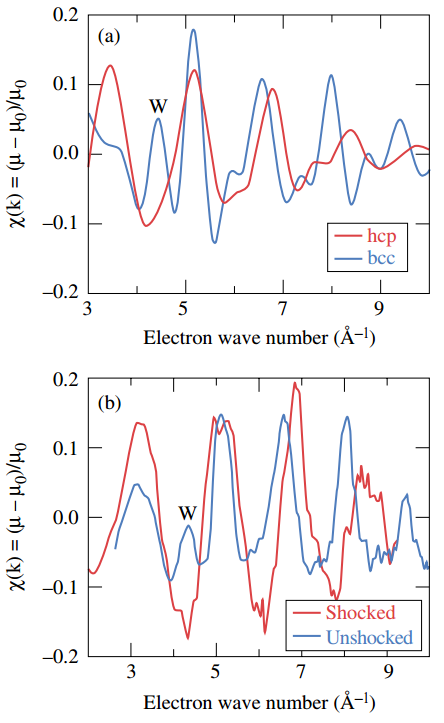
\includegraphics[scale=0.6]{../Figures/yaakobi_shock_xafs.png}
\end{figure}

XANES measurements on dense plasma have also been performed at laser plasma facilities. This requires narrower-band illumination compared with XAFS, which has been achieved using short pulse laser-driven multicomponent X-ray fluorescence backlighters. Levy et al., for example, have used this technique to demonstrate XANES-based thermometry based on measurement of the K-edge slope in Al isochorically heated to 3 eV. (cite Levy et al).

Laser wakefield accelerator X-ray sources generate fs-duration broadband X-ray emission, affording time resolution that surpasses what is possible with laser-driven backlighters. This makes wakefield accelerators especially well-suited to X-ray absorption spectroscopy of WDM generated at XFEL facilities (cite Albert). The combination of wakefield accelerators with XFELs promises the unprecedented possibility of XFEL pump-probe experiments with simultaneous fs-duration interrogation of the target using broad- and narrow-band hard X-rays. This combination also enables XAS measurements of low-Z materials, which is much more challenging at laser plasma facilities as a result of the mismatch between the short penetration lengths of x-rays near the K-edges of low-Z species and the relatively large target thicknesses (tens of microns) needed for effective laser ablation. 
% TODO  this paragraph sucks. 
% One appealing possibility is that of simultaneous XAS and XRD.
% TODO: use the figure from Albert et al., and cite it.

\begin{figure}[h] 
\caption{Parameter spaces of several x-ray techniques (X-ray phase contrast imaging (XPCI), x-ray absorption, and nuclear resonance fluorescence (NRF)), overlaid with curves indicating the regions of parameter space accessible by various x-ray source technologies and individual facilities (cite Albert).}
\label{albert_sources}
%(cite https://lasers.llnl.gov/science/icf/how-icf-works)}
\centering
\includegraphics[scale=0.5]{../Figures/albert_sources.png}
\end{figure}


\subsection{X-ray Emission and X-ray Fluorescence}
X-ray fluorescence spectroscopy (XRF) is an extensively used probe in experiments studying the interaction of high-intensity lasers with solid targets. In short-pulse laser experiments involving mid-Z elements heated to temperatures comparable to or larger than M-shell binding energies the ratio of $K_\beta$ to $K_\alpha$ emission is used as a measurement of temperature. Modeling the coupling efficiency between high-power laser and electrons in a solid-density target is of considerable significance to the effort to understand optical radiation-matter interactions at high laser intensities ($> 10^{19}$ W/cm$^2$); in this context, inference of target heating using $K_\beta/K_\alpha$ branching ratios provides a useful consistency check in the application of models to experimental data. (cite Myatt et all 2007, Nilson).

\begin{figure}[h] 
\caption{Experimental $K_\alpha/K_\beta$ ratios of emission from Cu foil heated by short-pulse lasers, with inferred electron temperature on the right vertical axis. Model calculations are heating for hot electron coupling efficiencies $\eta_e$ equal to 10\% and 30\% (cite Nilson)}
\label{fig:nilson}
%(cite https://lasers.llnl.gov/science/icf/how-icf-works)}
\centering
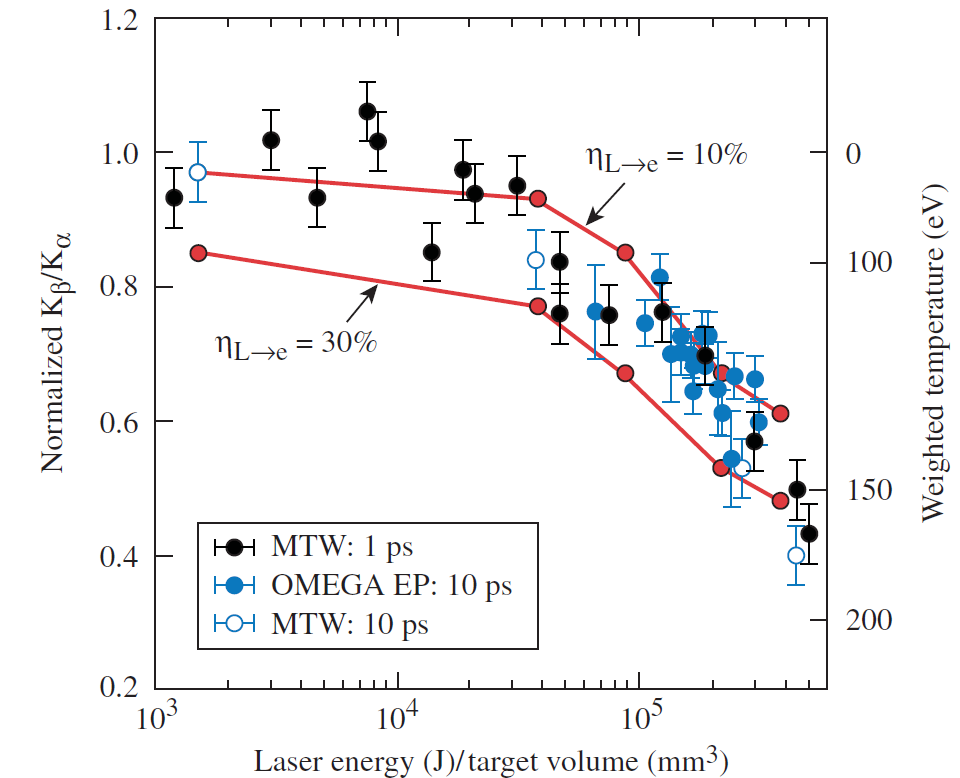
\includegraphics[scale=0.5]{../Figures/nilson_branching.png}
\end{figure}

X-ray emission spectroscopy (XES), the finer-grained cousin of XRF, provides more detailed information on the occupied density of states in a material and can be sensitive to valence-level excitations in the `tepid' transitional regime between ambient and warm dense matter states (cites). It has seen use primarily at XFEL facilities, where higher shot rates and probe intensities make the collection of datasets with satisfactory statistical quality easier. (cite photosystem 2 XES papers). The advent of XFELs as the first high-intensity, monochromatic, and tunable WDM probes has also enabled resonant inelastic X-ray scattering (RIXS) measurements, which has made possible the direct measurement of ionization potential depression on a fs timescale, as demonstrated by Vinko et al. (cite Vinko, Ciricosta.).

% K-U Plagemann, P Sperling, R Thiele, M P Desjarlais, C Fortmann, T D ̈oppner, H J Lee, S H Glenzer, and R Redmer. Dynamic structure factor in warm dense beryllium.  New Journal of Physics, 14(5):055020, 2012.


%In the high-momentum transfer Impulse Approximation of Eisenberger and Platzman, for example, XRTS becomes equivalent to Doppler-broadened Compton scattering, wherein the DDCS is proportional to an integral over the system's momentum-space density $\rho(p)$:
%
%\begin{equation}
%	\frac{d^2\sigma}{d\Omega d\omega} \propto \int d^3p \rho(p) \delta(p_q - (\omega m / q - \hbar q / 2)).
%\end{equation}
% TODO figure out what to do with section. How much detail is needed.


	% TODO: latex vectors?
	% TODO: cites. use either brian's thesis or same source as in the edxrd paper

	%The fundamental observable of XRTS is the dynamic structure factor $S(q, \omega)$ 


\section{Dissertation Outline}
% TODO sort out the name of UW Xap
The overarching theme in this thesis is the relationship, and frequent feedback, between scientific discovery and the development of new experimental techinique. To begin, in chapter 2 I introduce a scheme for single-shot measurement of the static structure factors of disordered dense plasmas produced at large-scale laser facilities such as Omega and NIF. In Chapter 3 I present an experimental observation of nonlocal heat transport by keV-scale electrons in a nanophase material and consider the question of how this effect can be used to improve WDM experiments conducted at XFELs via optimized nanostructured target design. In chapter 4 I discuss experimental results of a recent experiment at the LCLS in which we established bounds on the timescales for thermalization of the lattice in XFEL-heated metal oxides and measured the consequences of XFEL heating on electronic charge density, with subsequent comparisons to different model predictions.  In chapter 5 I describe an instrument-development effort toward a disposable CMOS-based X-ray camera for use in experimental environments hostile to electronics, particularly laser plasma facilities. Finally, in chapter 6 I introduce UW-XAP, a software tool for streamlined realtime data collection and analysis at the LCLS. 
 
\chapter{Physics of PENELOPE} % Main chapter title
This chapter serves as background material for Chapter 3 \ref{chap:hef_chapter}, in which we present the use of the Monte Carlo Code PENELOPE for the simulation of electron transport in nanostructured XFEL targets.

\label{Penelope} % For referencing the chapter elsewhere, use \ref{Chapter1} 

%----------------------------------------------------------------------------------------

% Define some commands to keep the formatting separated from the content 
%\newcommand{\keyword}[1]{\textbf{#1}}
%\newcommand{\tabhead}[1]{\textbf{#1}}
%\newcommand{\code}[1]{\texttt{#1}}
%\newcommand{\file}[1]{\texttt{\bfseries#1}}
%\newcommand{\option}[1]{\texttt{\itshape#1}}

%----------------------------------------------------------------------------------------

%Outline for this section.
%Context: splice this section into the HEF paper as part of an extended
%methods section. Before talking about PENELOPE I need to state what it
%is that we need to model, and with what accuracy.
%4. PENELOPE's treatment of the material-dependent energy-loss function.
%Discuss the program MATERIAL and justify penelope's use of Bragg's rule.
%May need to discuss the estar database?
% TODO: compare to the version of Dec 30 2016 (some changes were lost).
PENELOPE performs Monte Carlo simulations of coupled electron-photon transport in arbitrary materials in the energy range of 100 eV to 1 GeV. It uses a mixed simulation method that treats soft interactions (that is, those involving small angular deflections) with a multiple-scattering approach while individually simulating hard interactions. It is paired with a geometry-definition program, PENGEOM, that allows defining samples with volumes of different material composition separated by arbitrary quartic surfaces.

\section{Types of interactions}
In this section we consider the interactions that must be simulated to accurately model the spatial distribution of energy in a nanostructured target material heated by x-ray photons with energy on the order of 10 keV.
PENELOPE simulates the following interactions: electron scattering (elastic and inelastic), Bremsstrahlung emission, photon scattering (both elastic (Rayleigh) and inelastic (Compton)), photoelectric absorption and Auger emission, x-ray fluorescence, and pair production and annihilation. 
Figs. \ref{fig:sp} and \ref{fig:photon_sigma} show the energy dependence of the relative strengths of the above electron and photon interactions, respectively. 
Several of the processes have negligible or nonexistent roles on the $<$ 10 keV energy scale considered in the current work, allowing us to limit our scope to the electron scattering and photoabsorption (with consequent fluorescence and Auger emission).

\begin{figure}[h] 
\caption{Collisional and radiative electron stopping powers as a function of energy (cite)}
\label{fig:sp}
\centering
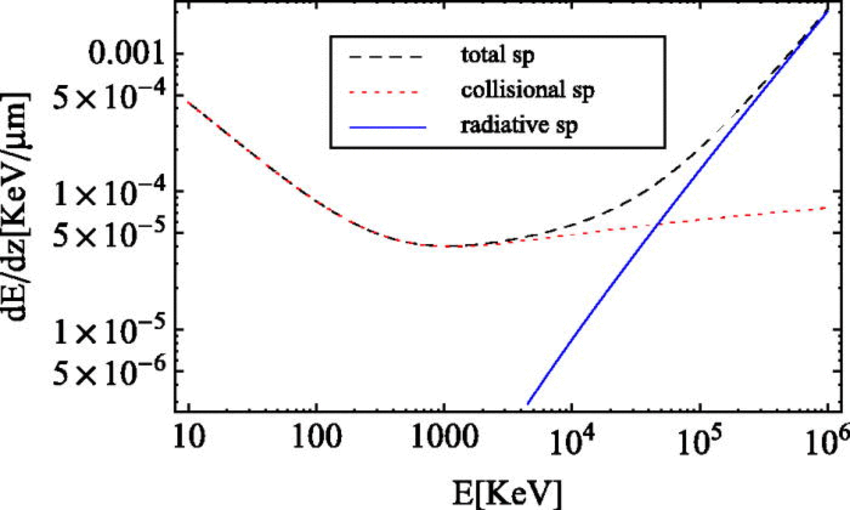
\includegraphics[scale=0.4]{../Figures/collisional_sp.png}
\end{figure}

\begin{figure}[h] 
\caption{Photon cross section components in C as a function of energy (cite Hubbell 1980)}
\label{fig:photon_sigma}
\centering
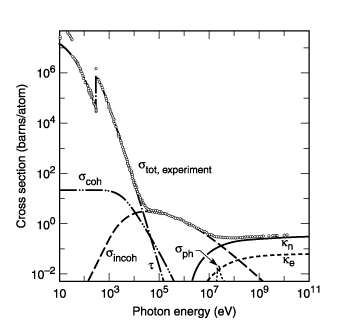
\includegraphics[scale=1]{../Figures/photon_sigma.png}
\end{figure}

In what follows we introduce the physics of photoabsorption and elastic and inelastic scattering with attention to each process's contribution to the spatial distribution of deposited energy in a relaxation cascade beginning with photoionization by a hard x-ray photon. We discuss standard modeling approaches relevant to the 100 eV--10 keV regime, with a focus on the aspects of PENELOPE's treatments most relevant to our regime of interest. % (including, for example, including relativistic energies).
%In the case of inelastic electron scattering, where numerous treatments of the central quantity (the generalized oscillator strength, or GOS) exist, we discuss necessary common features of all GOS models before introducing PENELOPE's specific treatment.

\subsection{Fluorescence}
Fig \ref{fig:photoionization} illustrates the photoionization of inner atomic shells and introduces the notation used to describe atomic energy levels and transitions between them.
Both the photoelectric effect and secondary (Auger) emission resulting from high-energy atomic excitations can be accurately modeled using established treatments that combine theoretical calculation of atomic states via self-consistent modeling (cite Pratt et al. 1973) with experimental data. Associated quantities are compiled in existing public databases; PENELOPE uses tabulated ionization energies from Carlson (cite Carlson et al.) and photoelectic cross sections from the LLNL Evaluated Photon Data Library (EPDL). The EPDL additionally provides emission probabilities for fluorescence photons and Auger electrons in the relaxation of ionized atoms to the ground state.

\begin{figure}[h] 
\caption{Atomic energy levels of the first three principal quantum numbers (left) and corresponding allowed radiative transitions (right).}
\label{fig:photoionization}
\centering
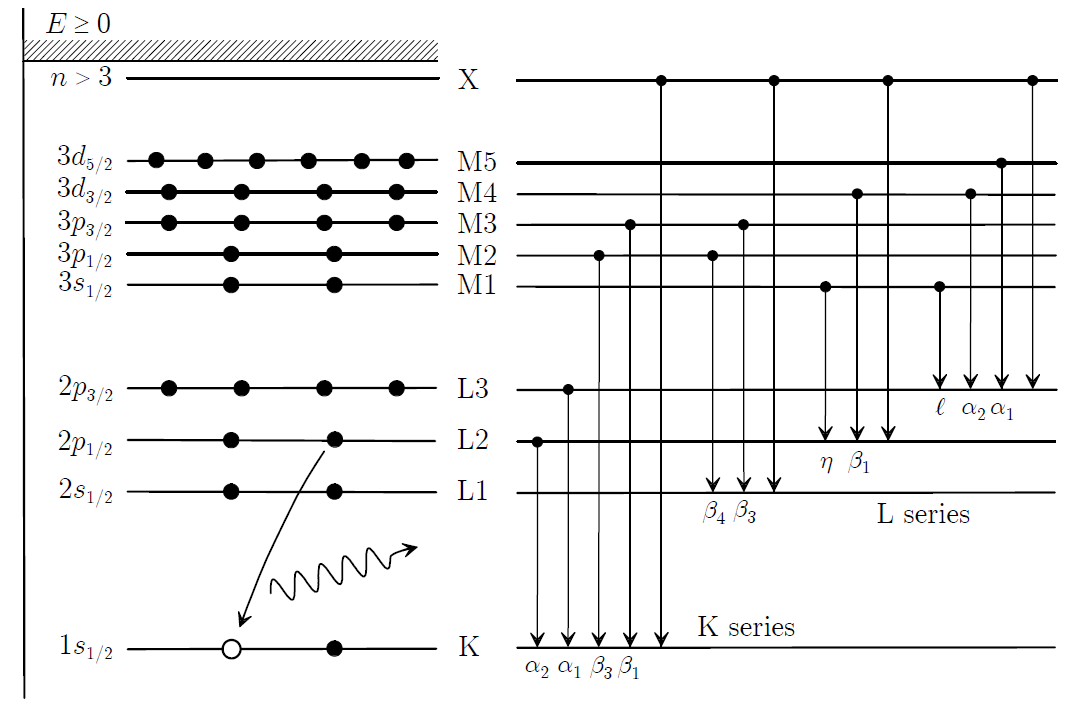
\includegraphics[scale=0.4]{../Figures/penelope_2_2.png}
\end{figure}



\subsubsection{Assumptions}
The above data sources are known to be accurate to the $1\%$ level above $1$ keV, under the condition (assumed by PENELOPE) of low incident photon densities, such that only single-electron transitions occur (cite PENELOPE manual).

% TODO: cite on the polarization dependence thing?
PENELOPE assumes that incident photons are unpolarized and consequently fails to reproduce the polarization-dependent angular distribution of emitted electrons. 
We note that it does incorporate the angular distribution from Sauter's (cite sauter 1931) treatment of relativistic photoelectron emission--which, however, reduces to isotropic emission in the nonrelativistic regime covered here.



\subsection{Elastic scattering}
Elastic scattering of electrons refers to interactions that do not alter target atoms' states. 
% TODO: consider moving some of the below text to the end of this section
%PENELOPE uses the static field approximation (cite Mott and Massey), which is accurate above energies of a few hundred eV (cite PENELOPE manual, page 102) but introduces a considerable error to the elastic DCS at and below 1 keV (discuss in next section). 
%An atom's electrostatic potential is expressed in terms of the nuclear and electronic charge densities, $\rho _n (r)$ and $\rho _e (r)$ respectively: 
%
%% TODO: nuclear charge should be a point
%\begin{multline}
%\phi (r) = e~4~\pi [\frac{1}{r}\int_0^{r}\rho(r')r'^{2} + \int_r^{\infty}\rho_n(r')r'dr'] -\\ e~4~\pi \frac{1}{r} \int_0^r\rho_e(r')r'^2 dr' + \int_r^\infty \rho_e(r') r' dr'].
%\end{multline}
%We note that, although PENELOPE accounts for the effect of the finite nuclear size on the elastic DCS, we simply treat the nucleus as a point source as this is sufficient for electrons with energy below 1 MeV. (cite PENELOPE manual)

%Fermi distribution:
%
%\begin{equation}
%\rho_n(r) = \frac{\rho_0}{exp[(r - R_n)(4ln3/t)] + 1},
%\end{equation},

%(cite Hahn et al. 1956 and understand the orgin of this expression)  $R_n$ is the mean radius and $t$ is the 'skin` thickness of $\rho_n$ defined in Hahn et al. 1956. 

%The total interaction energy for electrons is
%
%\begin{equation}
%V(r) = -e\phi(r) + V_{ex}(r),
%\end{equation}
%
%where $V_{ex}(r)$ is a local approximation of the exchange interaction between the incident electron and atomic electrons. The angular distribution of elastic scattering off this central field is axially symmetric, and the DCS $d\sigma_{el}/d\Omega$ may therefore be expanded into a sum of Legendre polynomials. [Citing Salvat 2005 or Walker, describe how the phase shifts are obtained from the Dirac radial wave functions. What's the role of the exchange term in all this?]

%\section{First view: Yukawa potential}
The simplest widely-used model for elastic scattering of electrons in a solid is the semi-classical approach of Wentzel and Lenz (cite Egerton p. 114 ), known as the Lenz model, which uses the Yukawa potential for the interaction between a fast electron and a target atom:

\begin{equation}\label{eq:yukawa} 
V(r) = \alpha^2 \frac{e^{-r/r_0}}{r}
\end{equation}

%sufficient to derive the approximate differential cross section of elastic scattering and to describe its influence on the spatial distribution of scattered electrons at our energy scale of interest. 

The first Born approximation gives the amplitude for a particle's scattering off of a spherically symmetric potential as
% TODO cite http://itp.uni-frankfurt.de/~valenti/SS14/QMII_2014_chap1.pdf or other

 \begin{equation}\label{born}
	f(\theta) \simeq -2 \frac{m}{\hbar^2 q} \int_0^\infty r V(r) \sin (qr)\, dr
\end{equation}

Substituting (\ref{eq:yukawa}) into (\ref{born}) yields 
%from http://itp.uni-frankfurt.de/~valenti/SS14/QMII_2014_chap1.pdf
%TODO: make the notation here consistent.
\begin{equation}
	f(\theta) \simeq -2 \frac{m \alpha^2}{\hbar^2 q} \int_0^\infty e^{-r/r_0} \sin (qr)\, dr = -\frac{2m\alpha^2}{\hbar^2 (r_0^{-2} + q^2)},
\end{equation}

therefore giving the following differential scattering cross section:
$$
\frac{d\sigma}{d\Omega} = |f(\theta)| = \frac{4 Z^2}{a_0^2 k_0^4} \frac{1}{(\theta^2 + \theta_0^2)^2},
$$
where $k_0 = m_0 v$ is the momentum of the incident electron, $\theta_0 = (k_0 r_0)^{-1}$ is the characteristic angle for elastic scattering and $a_0 = 4 \pi \epsilon_0 \hbar^2/m_0 e^2$ is the Bohr radius.

Using the Thomas-Fermi model, Wentzel and Lenz obtain $r_0 = a_0 Z^{-1/3}$ (cites). Doing this substitution and integrating over scattering angles gives
\begin{equation}
\sigma_e = \int_0^\pi \frac{d\sigma}{d\Omega} 2 \pi \sin \theta d \theta = \frac{4 \pi}{k_0^2} Z^{4/3}
\end{equation}

% TODO: copper->iron
We thus see that the angular deflections of elastic scattering decrease with increasing energy. For 10 keV electrons, $\theta_0 \simeq 0.1$ rad and $\sigma_e = 4.2 \times 10^{-20}~\mathrm{m}^2$. The elastic mean free path, an alternate measure of the collision frequency, is equal to $\lambda_e = 1/(\sigma_e n)$, where $n$ is atomic number density. As an example, inserting $\sigma_e = 39~\mathrm{\AA}^2$ and $n = 8.5\times 10^{25}/m^3$ for Fe yields $\lambda_e = 300$ \AA. The product of expected numbers of elastic collisions on typical transport length scales (whose values exceed 10 nm) and the characteristic scattering angle are therefore at least of order unity (in radians), demonstrating that elastic scattering has a substantial influence on the propagation of below--10 keV electrons.


Despite its simplicity, the Lenz model gives total cross sections to within 10 \% for light elements (cite Geiger 1964). For heavier species it underestimates the small-angle differential cross section (Fig. \ref{fig:e3.3}) but correctly reproduces the large-angle DCS.

\begin{figure}[h] 
	\caption{Angular dependence of elastic DCS of 30 keV electrons from a Hg atom under the Lenz model using the Wentzel potential (solid), and based on Hartree-Fock (dotted), Hartree-Slater (dot-dashed) and Dirac-Slater (dashed) wavefunctions.  (cite Egerton) }
	\label{fig:e3.3}
\centering
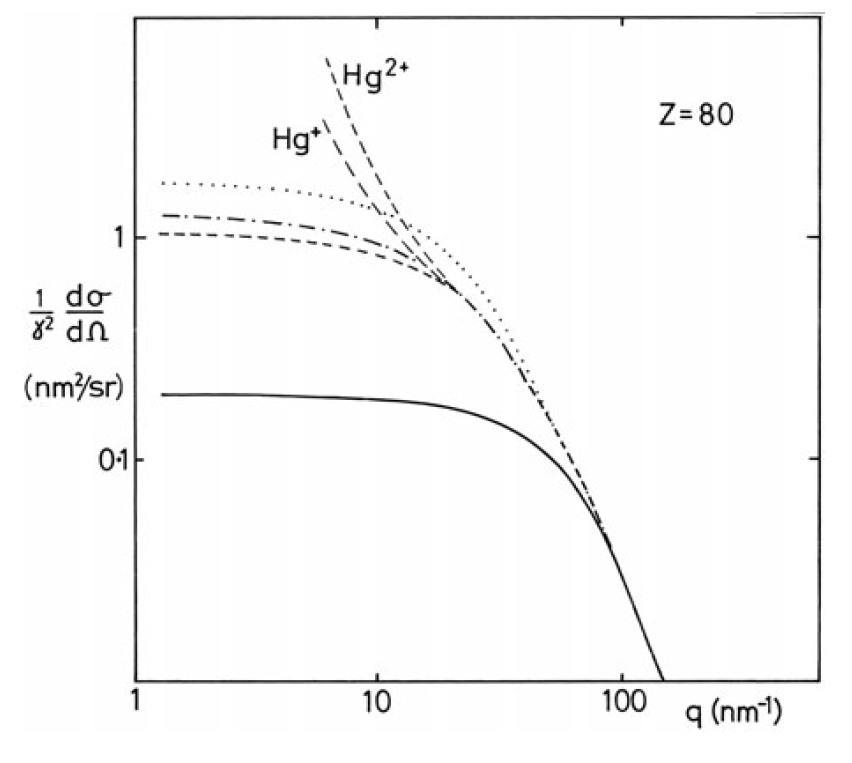
\includegraphics[scale=0.5]{../Figures/egerton_3_3.png}
\end{figure}

% reference title: applicability of the born approximation to collisions between electrons and excited atoms
More accurate approaches use iterative (e.g. Hartree-Fock) solutions to the Schroedinger or Dirac equations to solve for the atomic potential. (cite Rez 1984 or Starostin). Additionally, partial wave approaches can be used to avoid the Born approximation in regimes for which it fails (low electron energy and high-Z species). PENELOPE combines the above techniques: it solves the partial-wave expanded Dirac equation with a potential based on the Dirac-Fock electron density of Desclaux (1975, see citation on pg 102 of penelope manual) and exchange interaction of Furness and McCarthy (1973). We will elaborate on PENELOPE's modeling of elastic scattering only within the narrow concern of assessing its accuracy within the physical regimes that we simulate; for more detail the reader may refer to Chapter 3 of the PENELOPE manual. 


% Fig. (fig reference) shows the angular dependence of scattering for Fe. 

\section{Inelastic scattering}
We now discuss the treatment of inelastic collisions, which are the dominant mechanism for energy loss of electrons up to above 10 keV (Fig. \ref{fig:photon_sigma}).  In an atomic system, the differential cross section for a transition from initial state wavefunction $\psi_0$ to final state wavefunction $\psi_n$ is
%The double differential cross section for collisions with momentum transfer $q$ and energy loss $\omega$ is given by Fano (cite Fano 1963, see page 114 of PENELOPE manual) as

\begin{equation} \label{bornDCS}
\frac{d\sigma_n}{d\Omega} = \frac{m_0}{2\pi \hbar^2}^2 \frac{k_1}{k_0} \mid \int V(r) \psi_0 \psi_n exp(i q r) d\tau \mid ^2
\end{equation}
%TODO: fix the notation here. How does one do bolded text? dot products?
where $\textbf{k}_0$ and $\textbf{k}_1$ are the wave vectors of the incident electron before and after scattering and $q = \hbar (\textbf{k}_1 - \textbf{k}_1)$ is the corresponding momentum transfer. 

At nonrelativistic velocities the potential between electron and atom may be expressed as the following sum of Coulomb potentials of the nucleus and atomic electrons:

\begin{equation} \label{cpotential}
V(r) = \frac{Ze^2}{4\pi \epsilon_0 r} - \frac{1}{4 \pi \epsilon_0} \sum_{j = 1}^Z \frac{e^2}{\mid \mathbf{r} - \mathbf{r_j} \mid}
\end{equation}
%TODO
%(define whichever quantities haven't been introduced yet)
Substituting the second term of equation \ref{cpotential} into \ref{bornDCS}, we note that the nuclear potential is independent of the coordinates of the atomic electrons and can therefore be removed from the integral. The orthogonality of the wave functions $\psi_n$ implies that the nuclear potential does not contribute to inelastic scattering; the expression for the differential cross section of inelastic scattering is therefore:

\begin{equation} \label{inelasticDCS}
\frac{d\sigma_n}{d\Omega} = (\frac{4}{a_0^2 q^4}) \frac{k1}{k0} \mid \epsilon(q)\mid^2,
\end{equation}

where

\begin{equation}
	\epsilon_n = \int \psi_n \sum_j e^{i q r_j} \psi_0 d\tau.
\end{equation}


The generalized oscillator strength is an important related quantity:

\begin{equation}
f_n(q) = \frac{E_n}{R} \frac{\mid \epsilon_n(q)\mid ^2}{(q a_0)^2},
\end{equation}


where $R = (m_0 e^4 / 2)(4 \pi \epsilon_0 \hbar)^{-2}$, the Rydberg energy, and $E_n$ is the energy change of the transition. 

The GOS is in general continuous and therefore better expressed as a density with dimensions 1/energy, i.e. $df(q, E)/dE$, where $E$ is energy loss. This allows us to re-express the double-differential cross section of inelastic scattering as follows:

\begin{equation} \label{inelastic_DDCS}
\frac{d^2\sigma}{d\Omega dE} = {4 R}{Eq^2} \frac{k_1}{k_0} \frac{df}{dE}(q, E).
\end{equation}

%TODO: calculate a typical inelastic scattering cross section for comparison elastic scattering. The fact that the ratio is of order unity demonstrates that both matter.

\subsection{Dielectric function}
While this formulation makes it possible to calculate the GOS and associated quantities starting from atomic models, in solid state systems the scattering cross section of outer-shell electrons is influenced by collective effects and chemical bonding. It's therefore preferable to describe the inelastic scattering of an electron from a solid using the solid's dielectric response function, $\epsilon(q, E)$. 

Ritchie (cite Ritche 1957) showed, using Poisson's equation and Fourier transforms, that an electron moving in the z-direction in an infinite medium experiences a force of the following magnitude opposite its direction of motion: 


\begin{equation} \label{stp}
\frac{dE}{dz} = \frac{2\hbar}{\pi a_0 m_0 v^2} \int \int \frac{q_y E \Im[-1/\epsilon(q, E)]}{q_y^2 + (E/\hbar v)^2},
\end{equation}
% TODO: vectors?
where $q_y$ is the component of the momentum transfer vector perpendicular to $v$ and $\omega = E/\hbar$. This quantity is referred to as the stopping power. It can be expressed in terms of the previously-defined DDCS:

\begin{equation} \label{stp2}
\frac{dE}{dz} = \int \int n E \frac{d^2\sigma}{d\Omega dE} d\Omega dE,
\end{equation}

%\frac{d^2\sigma}{d\Omega dE} = 
where $E$ is energy loss and $\Omega$ is solid angle. By equating equations \ref{stp} and \ref{stp2} in the small-angle limit it can be shown, by comparison with the atomic treatment (cite), that 

$$
\frac{df}{dE}(q, E) = \frac{2E}{\pi E_a^2} \Im[\frac{-1}{\epsilon(q, E)}],
$$

thus demonstrating the equivalence of the atomic and dielectric approaches.

Note, finally, that the GOS fully determines the value of equation \ref{inelastic_DDCS} within the first Born approximation. As such, given the potential of equation \ref{bornDCS} all modeling of the inelastic scattering of electrons at intermediate energies (1 keV -- 300 keV) reduces to construction of a GOS model. 


%For a continuous energy loss spectrum, it takes the differential form $dF/dE(q, E)$, a density with respect to energy loss.

% TODO: move this somewhere
% We note that PENELOPE incorporates Fano's (1963) relativistic treatment of inelastic scattering of electrons in condensed media in place of the current treatment. 

\subsection{Modeling the generalized oscillator strength}
Analytical expressions for the GOS are known for only the two simple cases of the free electron gas and hydrogen atom. In practice, however, it has been shown that the physics of inelastic scattering is mostly determined by a few global features of the GOS (cite Salvat and Fernandez-Varea, 1992) and that relatively simple models are therefore adequate in most situations.


% TODO: fix the E/omega inconsistency
% TODO: read Salvat and Varea, 1992
The GOS is conventionally represented as a two-dimensional surface plot called the Bethe surface (Fig. \ref{fig:bethe}). 
We identify two constraints on the behavior of the Bethe surface which any GOS model must reproduce. First, in the limit $Q\rightarrow 0$, the GOS of the dielectric formulation becomes proportional to  the optical oscillator strength $\Im[-1/\epsilon(0, E)]$, which is experimentally constrained by x-ray emission measurements. Second, in the limit of large momentum transfer the most probable energy loss is equal to the kinematically-determined value for collision between two free electrons, $E = q^2/2$. (cite Sorini). The corresponding trace in energy and momentum is a feature of the Bethe surface known as the Bethe ridge.

% From 3.36 in Egerton book
\begin{figure}[h] 
\caption{Bethe surface for ionization of the K shell in C, based on a hydrogenic GOS model. (cite Egerton 1979)}
\label{fig:bethe}
\centering
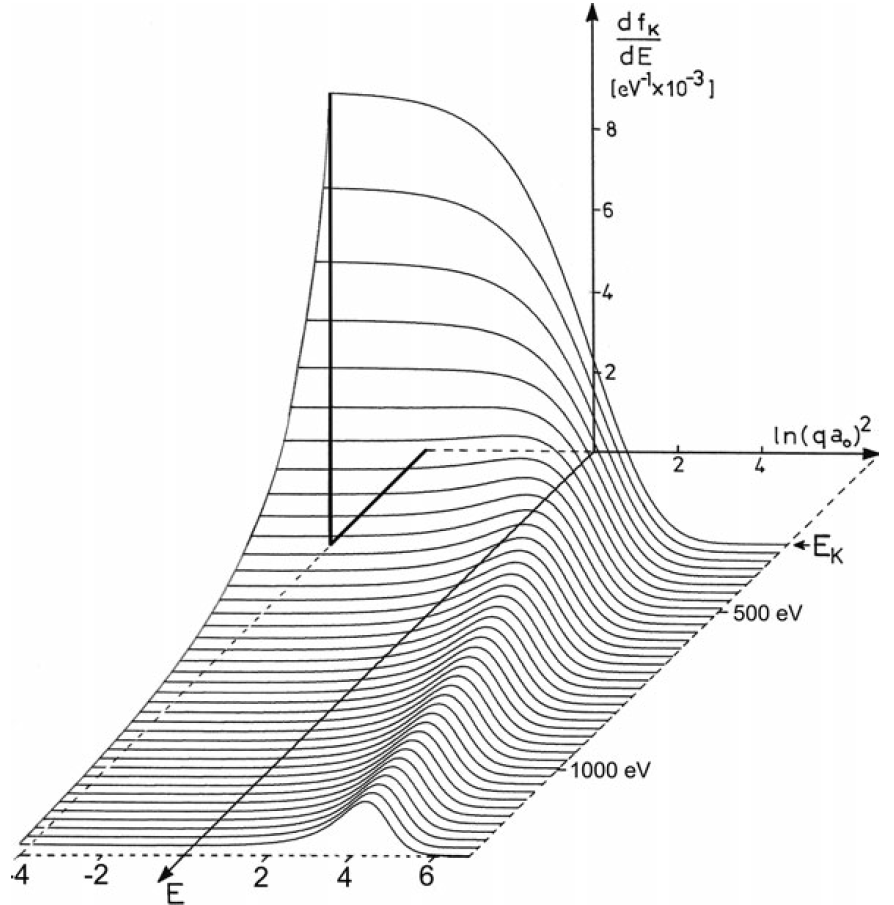
\includegraphics[scale=0.5]{../Figures/bethe.png}
\end{figure}

As in Compton scattering, the shape of cuts through the Bethe surface (i.e. spectra of scattered intensity as a function of energy at fixed momentum transfer) is determined by the momentum distribution of atomic electrons. Certain models, such as that of Sorini et al (cite Sorini 2006), derive a value for the width of the Bethe ridge from Fermi velocity calculations. PENELOPE adopts a simpler form based on the `$\delta$ -oscillator' model of Liljequist (cite Liljequist 1983) which splits the GOS into contributions from generalized `shells' (each corresponding to either an atomic shell or a collective excitation). The total GOS under this model is a sum over indices \emph{k} of the shells:

$$
\frac{df(q, E)}{dE} = \Sigma f_k [\delta(E - E_k) \Theta (q_k - q) + \delta(E-q) \Theta(q - q_k)],
$$
where for the \emph{k}th shell $f_k$ is the shell's number of electrons, $q_k$ is the cutoff recoil energy, and $E_k$ is the shell's resonance energy. $Q_k$ is equal to the shell's binding energy $U_k$ (excluding the conduction band, for which it is set to 0), and $E_k$ is computed from from $U_k$ and the material's mean electron density, following Sternheimer (cite Sternheimer 1952). Within this model the GOS is fully determined by the shells' occupations and cutoff (binding) energies $U_k$, which PENELOPE obtains from Carlson (cite Carlson 1975). It is possible, optionally, to direct PENELOPE to fit its GOS model to experimental stopping power data provided in material input files. It performs this fit through reweighting of the GOS model's oscillators .
% TODO (\emph{this is actually a guess, as the PENELOPE manual is totally opaque about how the GOS/DDCS is fit to stopping power input data. Better understanding would require me to revisit PENELOPE's code or contact the authors})

Substantial additional detail on the construction and interpretation of PENELOPE's GOS model can be found in its manual.

% TODO: talk about convergence with the Bethe model
% readily measured experimentally via the photoelectric cross sections in the diplole limit. (TODO: show this relationship between the photoelectric cross section and GOS mathematically, or cite Fernandez-Varea 1993 a). (cites. also, is this true (about the zero-angle energy loss spectrum?). Where Q is much larger than binding energies of the target electrons, the latter behave as though they were free and the GOS is described by the Bethe ridge, a peak along $W = Q$. 

% TODO numerical implementation and coarse graining
% TODO fluorescence
\section{Accuracy and useful regimes}
In the context of simulation of nanostructured materials, errors in PENELOPE's DCSs for electron scattering originate from both (1) the limited range of validity of PENELOPE's physical models with respect to the bulk properties PENELOPE seeks to reproduce, and (2) the difference between scattering DCSs of ambient-condition bulk materials on the one hand and high-temperature nanostructured materials on the other. We address these two issues separately.

\subsection{Nanophase dielectric functions}
% TODO: find and cite review article on surface plasmons in nano-materials
As mentioned previously, a material's inelastic scattering DCS is fully determined by its loss function, the imaginary component of the dielectric function. Any difference between the responses of bulk and nanophases arises from the contribution to the loss function of collective electronic excitations, i.e. plasmons. Plasmon modes in nanostructured materials are widely studied (cites), but there there has been little prior work in the context of high-temperature dense matter. The question of collective electronic excitations in heated nanophase materials thus manifests itself as both a problem and an opportunity. On the one hand, the lack of experimental data and accurate modeling makes it impossible to fully quantify the inaccuracy of simulations of ambient, bulk materials. On the other hand, XFEL heating experiments could be used to discriminate between computed dielectric response functions and their underlying finite-temperature electronic structure modeling--to the extent that alternative models generate experimentally measureable differences in the inelastic DDCS. We thus suggest that XFEL heating of nanostructured materials could enable a joint modeling/experimental program to validate WDM electronic structure theory.

\subsection{Numerical bound on low-energy loss DCS uncertainties} \label{ledcs}
In the current situation, wherein the plasmon contribution to the loss function is not known, we can take advantage of the fact that plasmon resonance are confined to energy losses smaller than approximately 100 eV. The influence of the low-energy region of the loss function on the spatial distribution of deposited energy can therefore be bounded using the continuous slowing down approximation (CSDA) of 100 eV electrons. The CSDA for electrons of energy $E_0$ is the following integral over stopping power: 

$$
l_{CSDA} = \int_{E_{final}} ^ {E_0} (\frac{dE}{dz})^{-1},
$$
where $E_{final}$, the final energy of the electron, is usually taken to be 10 eV. For elements heavier than boron, $l_{CSDA} < 10$ nm for $E = 100$ eV. We therefore conclude that inaccuracy in treatments of collective excitations affect the spatial distribution of energy deposited by electrons only at a length scale below 10 nm (Fig. \ref{fig:csda})% (\hyperref[cite]{http://xdb.lbl.gov/Section3/Sec\_3-2.html}) 

\begin{figure}[h] 
\caption{CSDA range as a function of energy for several materials, based on computed low-energy stopping powers. (cite LBL X ray data booklet and associated papers)}
\label{fig:csda}
\centering
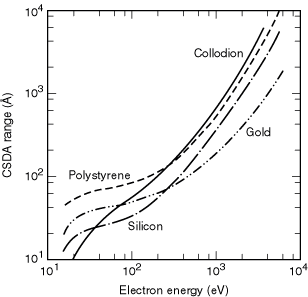
\includegraphics[scale=0.7]{../Figures/csda.png}
\end{figure}

\subsection{Energy cutoffs} \label{cutoffs}
PENELOPE stops simulation of an electron's motion once its energy drops below a prescribed cutoff value; at the endpoint of an electron's simulated track all of the electron's final energy is deposited at its final position. The resulting distortion in the spatial distribution of deposited energy can be bounded, as above, using the CSDA. PENELOPE's cutoff energy can be set as low as 50 eV. Assuming this value is chosen, the resulting error is smaller than the bound established in section \ref{ledcs} on error attributed to inaccuracy in the low-energy dielectric function. Simulation error due to PENELOPE's energy cutoff can therefore be safely neglected.

% TODO: see berger and seltzer 1982 calculation of mean excitation energies
\subsection{Elastic scattering}
% TODO also need to talk about the absorption correction / dual channel thing
PENELOPE's use of the static field approximation in its elastic scattering model introduces a low-energy error in the DCS due to the effect of the polarizability of atomic charge (cite Salvat 2003). The size of this error is 20\% at 1 keV and 50\% at 100 eV (PENELOPE manual, pg. 102). The CSDA range at 1 keV, where uncertainty at the level of the DCS is considerable, ranges from 10 nm for high-Z elements to over 100 nm for low-Z ones. Because the results of the PENELOPE simulations discussed in Chapter \ref{hef}  are sensitive to errors on the 10 nm - 100 nm length scale, the CSDA does not usefully constrain the elastic DCS model's contribution to uncertainty in the spatial distribution of deposited energy. 

The magnitude of uncertainty in the elastic DCS may be calculated by modeling elastic scattering of an electron as a correlated random walk defined by an elastic collision mean free path $\lambda_e$ and energy-dependent distribution of scattering angles. Cursory consideration suggests that closed form solutions for transport distances are available only under restrictive assumptions; implementing this calculation as a Monte Carlo simulation appears straightforward, but we have not done so. It is worthwhile pursuing in the future, since until then one cannot fully quantify total uncertainties in PENELOPE's energy transport predictions. 

%characteristic scattering angle $\theta_0$, the number of steps after which the electron's direction of motion becomes uncorrelated with its initial direction is of the order $n = \pi/\theta_0 \lambda_e$. The number of elastic scattering events an electron experiences as it slows from an energy of 1 keV to 100 eV (the previously-established--but arbitrary--cutoff below which the treatment of section \ref{ledcs} applies) is
%
%sketch: basically I have to calculate the number of scattering events, and associated dephasing of the electron's direction, for several `bins' of energy between 100 eV and 1 keV. For each bin we calculate the equivalent number of steps under an uncorrelated random walk. This yields an expected displacement proportional to the square root of the number of steps in the uncorrelated random walk, which we can multiply by the elastic DCS uncertainty in order to get an associated displacement uncertainty. All displacement uncertainties can then be added in quadrature, yielding a final uncertainty. 


\section{Inelastic scattering}
% TODO In the prior discussion of scattering models I need to add the equation for the inelastic/elastic scattering ratio and also compare characteristic scattering angles.
Inelastic scattering has much smaller characteristic angles than elastic scattering scattering but comparable total cross sections. As a result the influence of angular deflections by inelastic scattering on the propagation of electrons is relatively small. The effect of uncertainties in the inelastic scattering DDCS can thus be neglected, and we confine our attention to uncertainty at the level of the stopping power, a more coarse-grained quantity.

Fig \ref{fig:stp_accuracy} compares PENELOPE's computed stopping powers and inelastic mean free paths for Al to several experimental datasets. The level of disagreement between different datasets is of the order 2 in the 1 keV - 10 keV energy loss range; the discrepancy between PENELOPE's modeled stopping power and the experimental datasets is also of this order. Because all transport lengths are proportional to stopping power we must thus contend with a factor of 2 uncertainty in the length scale of computed spatial distributions--far larger than any of the other uncertainties we have considered until now. 

The conclusions of Chapter \ref{hef} can nevertheless be conserved, with one modification, if we consider PENELOPE's error in modeling the 1 - 10 keV stopping power as an unknown constant-factor scaling in stopping power. Such an uncertainty corresponds to an unknown scaling of both (1) the length scale of spatial distributions of deposited energy and (2) the flux magnitude of nonlocally-transported energy crossing a given material interface. To give a simple illustration, consider a one-dimensional configuration consisting of an infinite extent of source material from $x = -\infty$ to $x = \infty$. When the sample receives x ray illumination of magnitude unity at position $x0$ the density distribution $\rho(x)$ of deposited energy is given by a response function $f(x)$ (fully determined by the sample material's stopping power and incident x-ray spectrum): $ \rho(x) = f(x - x0) $. If the material is uniformly illuminated by x rays in the region spanning $x = 0$ to $x = \infty$ then (in arbitrary units):

$$
\rho(x) = \int_0^{\infty} f(x - x') dx'.
$$

Under the substitution $f(x) \rightarrow g(x) = f(c x)$ (equivalent to scaling $dE/dz \rightarrow (1/c) dE/dz$ of the stopping power), and maintaining normalization of the response function, the distribution becomes:

% TODO: there's something wrong here
$$
\rho'(x) = \int_0^{\infty} c f((c (x -  x'))) dx = \int_{cx}^{\infty} f((u)) u.
$$

Therefore constant-factor scaling of the stopping power is equivalent to a change in units of length, implying that, under our assumed form of the uncertainty in $dE/dz$, and adding the assumption that the unknown scaling factor $c$ is equal for all materials, the simulated spatial distributions of deposited energy density are correct up to a uniform scaling of the sample geometry. 

%all the modeling error is captured by deviations in the stopping power.



\begin{figure}[h] 
\caption{Stopping power and inelastic mean free path for electrons as a function of energy in Al calculated by PENELOPE and from several experimental datasets (cite Fernandez-Varea et al., 1993)}
\label{fig:stp_accuracy}
\centering
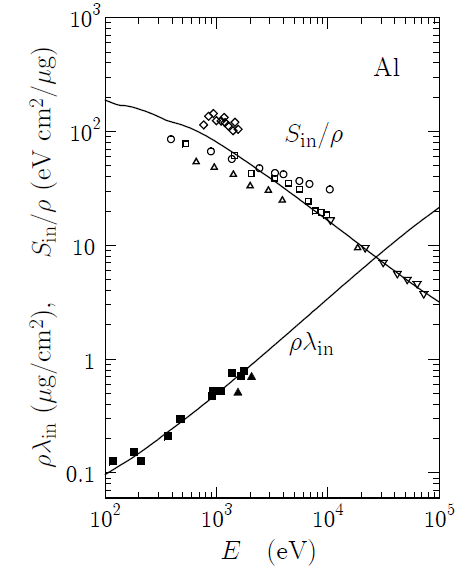
\includegraphics[scale=0.7]{../Figures/penelope_3_11.png}
\end{figure}

\section{Dosimetry}
PENELOPE's dosimetry includes both linear energy transfer from radiation to matter and the contribution of particle track ends, as mentioned in section \ref{cutoffs}. At the energy scales of interest the former contribution may be neglected, and the distribution of energy deposited by a particle shower is entirely dependent on simulated inelastic scattering events. PENELOPE's dosimetry calculation is tied to the termination of electron tracks: when an electron's energy drops below the (previously-defined) cutoff value its simulation ceases, and its entire energy is deposited at the track's endpoint.  Similarly, the energy loss of soft inelastic collisions (ones having energy loss greater than the cutoff energy $W_{cc}$) is deposited locally (whereas hard inelastic collisions generate secondary electrons that are individually tracked). 

Coarse-graining of the dose distribution is done by dividing the simulation volume into a three-dimensional grid of cells, in each of which PENELOPE calculates the total dose of deposited energy. This grid is defined by the parameters GRIDX, GRIDY, GRIZ and GRIDBN in PENELOPE's input.

These spatial dose distributions are the output data of interest in the simulations of Chapter \ref{hef}.


\chapter{Nonlocal Heat Transport and Improved Target Design for X-ray Heating Studies at X-ray Free Electron Lasers}
\label{chap:hef_chapter}

Oliver Hoidn and Gerald T. Seidler\textsuperscript{(*)}

Physics Department, University of Washington, Seattle WA

(*) seidler@uw.edu

The extremely high power densities and short durations of single pulses
of x-ray free electron lasers (XFELs) have opened new opportunities in
atomic physics, where complex excitation-relaxation chains allow for
high ionization states in atomic and molecular systems, and in dense
plasma physics, where XFEL heating of solid-density targets can create
unique dense states of matter having temperatures on the order of the
Fermi energy. We focus here on the latter phenomena, with special
emphasis on the problem of optimum target design to achieve high x-ray
heating into the warm dense matter (WDM) state. We report fully
three-dimensional simulations of the incident x-ray pulse and the
resulting multielectron relaxation cascade to model the spatial energy
density deposition in multicomponent targets, with particular focus on
the effects of nonlocal heat transport due to the motion of high energy
photoelectrons and Auger electrons. We find that nanoscale high-Z/low-Z
multicomponent targets can give much improved energy density deposition
in lower-Z materials, with enhancements reaching a factor of 100. This
has three important benefits. First, it greatly enlarges the
thermodynamic parameter space in XFEL x-ray heating studies of lower-Z
materials. Second, it allows the use of higher probe photon energies,
enabling higher-information content X-ray diffraction (XRD) measurements
such as in two-color XFEL operations. Third, while this is merely one
step toward optimization of x-ray heating target design, the
demonstration of the importance of nonlocal heat transport establishes
important common ground between XFEL-based x-ray heating studies and
more traditional laser plasma methods.

Submitted April 2017 Physical Review B

\section{I. Introduction}

Dense matter under extreme conditions of pressure (P), temperature (T),
or both, is a topic of classic and growing interest across multiple
subfields of contemporary science. {[}1-5{]} We focus here on the very
specific case of femtosecond-scale x-ray heating of crystalline matter,
in which there is growing evidence that the lattice often has limited
opportunity to structurally relax during the incident x-ray pulses
{[}6-8{]} and that the loss of crystallinity during the x-ray pulse may
have only modest scientific impact. {[}9{]} Such studies hold a
significant and, we propose, unique position for discovery, because they
encompass the case in which the consequences that traditional condensed
phase electronic structure theory has on the structure of
partially-ionized plasmas will be strongest and most easily
interrogated. Hence, the study of crystalline matter at ambient density
but highly elevated electronic temperature holds high potential for
directly testing foundational issues in finite-T density functional
theory, especially including the proper treatment of T-dependent
functionals. {[}10-12{]}

This point has recently been made by Valenza and Seidler {[}12{]}, who
demonstrated that finite-T DFT makes strong, initially counter-intuitive
predictions about the evolution of the absolute and relative Bragg peak
intensities in x-ray diffraction (XRD) from crystalline matter as a
function of electronic temperature on the 1 -- 50 eV scale. The key
point is that XRD provides a more detailed interrogation of the
population of electronic states for crystalline matter than it does for
the more amorphous states interrogated after, e.g., laser shock heating.
Furthermore, it is this temperature dependence that is a key
\emph{microscopic} \emph{observable} of all finite-T DFT approaches: the
central quantity calculated in DFT is, after all, the spatial
distribution of electron density. Therefore, careful characterization of
the real-space charge density at elevated electronic temperatures in a
cool lattice gives a direct path to evaluating different DFT
implementations. This is particularly significant as regards the
temperature-dependent exchange functional, which is essential to
predictions of bulk thermodynamic and elastic properties {[}10,11,13{]}.

However, in such a research program there is a confounding detail. The
most effective heating by x-rays will occur with lower-energy photons
(that are more strongly absorbed) whereas any detailed interrogation of
the real-space charge distribution by XRD requires the use of higher
energy x-rays to obtain information over a wide momentum transfer range.
{[}12{]} This dilemma raises a question that is new in the XFEL
community but old in the broader plasma physics community: \emph{Given
the incident pulse characteristics and the desired sample material, how
does one design a target to achieve optimal energy density deposition}?

The most comprehensive treatment of this question would include a fully
spatio-temporal treatment of radiative transport as well as electronic
dynamics and electron-atom interactions wherein, again because of the
short time scales, lattice relaxation can be ignored or at least is
secondary. Within this framework, the temporal evolution of
electron-electron and electron-atom interaction includes several stages.
First, the atomic physics of the core levels gives rise to an initial
population of high-energy Auger electrons and photoelectrons that decay
into low-energy (\textless{} 50 eV) electronic excitations (both
collective and single-particle) on the scale of a few femtoseconds. The
resulting collective excitations decay by generating electron-hole pairs
on the time scale of tens of femtoseconds. Subsequent electron-electron
thermalization occurs on the scale of 100 fs -- 1 ps for ambient matter
{[}14-17{]}, but in general has a strong eV-scale temperature
dependence, thus requiring a self-consistent treatment at high incident
flux levels.{[}15{]}

Here, we take a simpler approach with the goal of identifying and
illustrating the most important contributors to x-ray heating and how
their spatial extent strongly influences optimum x-ray heating target
design, in the limited sense of optimizing the deposited net energy
density in the desired sample phase. Specifically, we address the key
questions surrounding nonlocal energy transport by hot electrons. This
topic has a long history in plasma physics, especially for inertial
confinement fusion target design, but enters here with typically
lower-energy electrons, i.e., keV-scale, than are important in ICF and
in direct-drive laser-heating studies. This causes the energy deposition
length of the hot electrons to decrease from the 100-1000 µm scale for
MeV electrons in laser experiments to instead only
$\sim$50-200 nm, depending on the atomic number of the
species present in the XFEL x-ray heating target.

It is this much shorter length scale that brings us to consider
multicomponent nanoscale targets for x-ray heating so that the influence
of nonlocal energy transport by the hot electrons can be usefully
engineered. While the importance of nanoscale energy transport has not
previously been discussed in the context of XFEL heating target design,
it has been studied and exploited in other experimental contexts. For
example, there exists a significant body of literature in the medical
physics community concerned with using gold nanoparticles for dose
enhancement in radiotherapy treatment. {[}18,19{]} A contrasting
application of nonlocal energy transport is found in the macromolecular
crystallography community, where there is interest in the use of
submicron incident x-ray beams so that a large fraction of high-energy
electrons escape the beam spot before slowing down, thus reducing
radiation damage in the probed sample volume. {[}20-24{]}

With the above context established, we consider here a nanostructured
target design that enhances energy deposition in a sample material using
nonlocal heat transport from a more strongly x-ray absorbing material in
contact with the sample -- we refer to this second material as a
`cladding' as a matter of convenience, for closer contact to the
terminology of laser-shock target design, even when the geometry may not
strictly be cladded. Fig. \ref{fig:hef_image1} sketches several corresponding geometries,
but in the current paper we concentrate on the particularly simple one
of Fig. \ref{fig:hef_image1} (c), consisting of a single thin film of sample material clad
with Au. We use the Monte Carlo code PENELOPE to simulate
three-dimensional electron-photon transport and the corresponding
spatial distributions of deposited energy to demonstrate two benefits to
the design: first, it significantly enhances in-sample energy
deposition, and second, it relaxes constraints on XFEL pump photon
energy in a way that substantially increases the information content of
XRD measurements in certain experimental contexts.

We proceed as follows. In section II, we describe the methods used to
simulate photoionization and electron transport in a nanostructured
target and discuss the simplifying approximations on which we rely. In
section III, we present and discuss simulation results of multilayer
targets consisting of sample material clad on one or two sides with
gold. We find that such a cladding configuration significantly increases
deposited energy density in a sample material, with the largest
enhancement in low-Z samples. We argue that this enhanced effect in
low-Z samples opens the door to wide-angle x-ray diffraction (wide-angle
XRD), with significant utility for studying the time dynamics of the
energy relaxation cascade for both electronic and lattice/ion degrees of
freedom in such materials. These observations are particularly relevant
in the context of two-color x-ray pump x-ray probe experiments at
XFELs{[}25-29{]}, but also serve more generally to establish the
importance of nanoscale nonlocal heat transport in high-intensity XFEL
studies. Finally, in section IV we conclude.

\section{II. Methods}

The simulation of electron transport in condensed matter is an area of
ongoing research. In addition to continuing development of
well-established codes in the high-energy experimental particle physics
community {[}30,31{]}, new developments include incorporation of
\emph{ab initio} band structure calculations in order to accurately
model the electron mean free paths of interband transitions and plasmon
excitations from relativistic energies down to a few eV. {[}32,33{]}

In the regime relevant to the present study, calculation of the spatial
distribution of deposited energy caused by absorption of a hard x ray
requires accurate treatment of the processes that describe scattering of
photo- and Auger electrons at the 100 eV to 10 keV scale (generation of
secondary x-ray photons, though present, plays a negligible role in
energy transport). The simplest atomic treatments of elastic and
inelastic scattering demonstrate that, for mid- and high-Z elements, the
ratio of elastic to inelastic total cross sections is of order unity and
that characteristic elastic scattering angles are sufficiently large
(for instance, of order 1 rad for $\sim$1 keV electrons) to
influence deposited energy distributions. {[}34{]} Both components,
therefore, must receive accurate treatments to adequately model spatial
energy deposition distributions in a nanostructured target.

The spatial distribution of deposited energy is determined by the
electron stopping power \(\frac{\text{dE}}{\text{dz}}\), which in a
classical treatment is related to a material's dielectric function
\(\varepsilon(q,\ \ \omega)\) by

\begin{quote}
\(\frac{\text{dE}}{\text{dz}} = \ \frac{2^{2}}{\pi a_{0}m_{0}v^{2}}\ \iint_{}^{}\frac{q_{y}\omega\ Im\lbrack\frac{- 1}{\varepsilon(q,\ \ \omega)\rbrack}}{{q_{y}}^{2} + \left( \frac{\omega}{v} \right)^{2}}dq_{y}d\omega,\)
(1)
\end{quote}

where ω is angular frequency, \(q\) is momentum transfer (with \(q_{y}\)
the magnitude of the component for momentum transfer perpendicular to
the z-direction), \(a_{0}\) is the Bohr radius, \(m_{0}\) is the
electron mass, and \(v\) is the electron velocity. {[}34{]} In the case
of electron showers generated by 5-10 keV photons, the electron stopping
power's dependence on \(v\) causes nonlocal energy transport to be
dominated by the highest-energy Auger and photoelectrons. Though the
slower time evolution of the subsequent electronic and lattice dynamics
may be neglected in the present context of simulating fsec-scale energy
transport, the possibility of interrogating it by time-resolved XFEL
pump-probe measurement is an interesting topic in its own
right.{[}25,26{]}

To model the above physics we used the code PENELOPE, which implements
particle-tracking Monte Carlo simulations of electron showers generated
by x-ray photoionization.{[}31{]} PENELOPE uses total and differential
cross sections based on several physical models. Briefly, it derives
elastic and inner-shell inelastic cross sections from strictly atomic
wave functions, while the valence contribution to the inelastic double
differential cross section is based on the Born approximation and
generalized oscillator strength model of Liljequist {[}35,36{]}, with an
energy loss-dependent normalization that allows the model to replicate
empirical stopping power data (provided as program input). Although the
inelastic scattering cross section is dominated by low-energy loss
collisions, inner shells contribute the majority of the stopping power
for several-keV electrons, which account for the longest-range energy
transport. For electrons of those energies the stopping power of a
compound may be approximated within five percent by a stoichiometric sum
based on atomic treatments of its constituents (an observation referred
to as Bragg's rule). {[}37{]} Consequently we employed material data
files generated by the PENELOPE 2011 program MATERIAL, which applies
this approximation to infer stopping powers of arbitrary compounds using
data from the NIST ESTAR database. {[}31,38{]}

\section{III. Results and discussion}

We now present results for several realizations of our nanostructured
target design, all of which consist of thin films clad with Au on one or
both sides. The heating of an Fe thin film via nonlocal heat transport
by hot electrons is illustrated in Fig. \ref{fig:hef_image2}, which shows a two-dimensional
projection of electron trajectory traces in an Au-Fe-Au trilayer
stimulated with 7 keV incident photons. The color-coding of the tracks
shows that, due to the much larger number of photoexcitations in the Au
cladding compared to Fe inclusion, most hot electrons propagating in the
Fe are part of a photoionization relaxation cascade originating in the
cladding. Inelastic scattering of these hot electrons is the dominant
contribution to energy deposition in the central Fe region, as
quantified by Fig. \ref{fig:hef_image3}, which compares the linear energy deposition of
several Au-Fe-Au trilayer configurations to that in bare Fe.

Photoionization by 7 keV photons yields mean energy deposition lengths
\(l\) of 15.0 nm and 35.3 nm, respectively, in simulated bare Fe and
bare Au targets, where
\(l = \ \int_{z = 0}^{\infty}{z(\overrightarrow{r})\ \rho\left( \overrightarrow{r} \right)\ d^{3}\overrightarrow{r}}\),
with \(\rho\left( \overrightarrow{r} \right)\) the volume density of
deposited energy and \(z\) the magnitude of the projection of
\(\overrightarrow{r}\) onto a fixed, arbitrary unit vector. Consistent
with the above characteristic lengths, we found that absorbed energy
density in the Fe inclusion saturates beyond an Au cladding thickness of
50 nm. Fig. \ref{fig:hef_image3} (a) shows the deposited energy distribution in a bare
Fe\textsubscript{3}O\textsubscript{4} target and in several Au-
Fe\textsubscript{3}O\textsubscript{4}-Au trilayers with varying
thicknesses of the Fe\textsubscript{3}O\textsubscript{4} inclusion. An
interior layer thickness of 50 nm results in a factor of five
enhancement in deposited energy density relative to the bare
Fe\textsubscript{3}O\textsubscript{4} target. The increase in deposited
energy density in a clad sample compared to a bare one is significantly
larger for lower-Z materials, reaching a factor of 100 for an Au-C-Au
target of the same geometry (Fig. \ref{fig:hef_image4}).

These enhancements in energy deposition increase the accessible
thermodynamic parameter space in all XFEL heating experiments, which is
particularly significant for experimental diagnostics that require
deviation from optimal pump pulse characteristics and are therefore
normally incompatible with heating studies, for instance XRD. We
illustrate this in Fig. \ref{fig:hef_image5}, which compares the energy deposition in
Au-Fe-Au and Au-Fe\textsubscript{3}O\textsubscript{4}-Au targets
stimulated with photons below the \emph{K}-edge of Fe to that in a bare
Fe target heated by photons above the edge. Nonlocal heating of the
former samples compensates for the reduction in sample heating caused by
lowering the incident photon energy below the Fe \emph{K}-edge; the
multicomponent targets thus allow improving the ratio of signal to
(fluorescence) background while---in the more favorable case of
Fe\textsubscript{3}O\textsubscript{4}--maintaining an energy deposition
density comparable to the highest level possible with an equivalent
monolithic target. However, Fig. \ref{fig:hef_image6} also demonstrates a tradeoff of the
cladding's presence: the diffracted signal from Au is stronger than that
from the sample, making the described reduction in background worthwhile
only assuming sufficient separation between Bragg peaks of the sample
and cladding.

Low-Z sample materials provide a separate, independently interesting,
case for the use of structured target design in XRD studies. In such
materials, nonlocal heat transport is effective over a much wider range
of incident photon energies compared to direct x-ray absorption. Until
now, x-ray heating studies of low-Z materials, such as graphite, have
required incident photon energies below 3 keV to reach HED conditions
(\textgreater{} $\sim$1 eV temperatures) due to these
materials' small photoelectric cross sections in the hard X ray (photon
energy \textgreater{} 5 keV) regime. This restriction limits the
kinematically accessible range of momentum transfers in XRD, which
correspondingly reduces available information on real-space charge
density.

This creates an experimental dilemma with scientific consequences. For
example, Hau-Riege et al.{[}39{]} showed evidence for ultrafast melting
of graphite during a 40 fs-long XFEL pulse but were limited, for the
reason described above, to using 2 keV incident photons, yielding
diffraction from only the 002 Bragg reflection of graphite. The authors
interpreted quenching upon heating of the 002 peak as evidence of
nonthermal lattice melting. However, Valenza \emph{et al.}{[}12{]}
questioned this conclusion based on simulated diffraction using
frozen-core finite-T DFT calculations, which predicted strong quenching
of the graphite 002 reflection due to purely electronic reorganization
in crystalline graphite at 10 eV electronic temperature. In graphite and
other low-Z systems, the only means of unambiguously separating lattice
disorder from electronic heating in the XRD signal is to probe several
Bragg peaks, including the lowest-order reflections and their harmonics.
{[}12{]}

It is therefore interesting to ask whether high energy-densities can be
achieved in graphite when using photons suitable for wide-angle
scattering. In Fig. \ref{fig:hef_image4} we show the deposited energy densities in Au-C-Au
trilayers of several interior thicknesses, once again using 7 keV
incident photons (sufficient to probe the 006 reflection of graphite).
The deposited energy density in the interior layer is at least a factor
of 100 greater compared to an unclad sample with the same incident
photon energy, and a factor of two greater compared to an unclad sample
stimulated with 2 keV photons. Indirect heating via high-Z cladding thus
eliminates the constraint of selecting incident photon energies near a
low-Z material's small core binding energies, making wide-angle XRD
possible. In the context of carbon, the weakness of the XRD from C
compared to Au can be uniquely compensated with a highly-oriented
pyrolytic graphite (HOPG) sample, whose high-reflectivity 00\emph{l}
peaks yield much higher signal to background ratios than the powder-like
Bragg and thermal diffuse scattering of polycrystalline Au. Similar
configurations exploiting mosaic or single-crystal samples may enhance
wide-angle XRD on a variety of low-Z systems, offering a much-improved
ability to experimentally test predictions of finite-T DFT-based
modeling of electronic structure in low-Z condensed matter, where
finite-T effects are easiest to identify because of the relatively large
valence-electron contribution to the XRD signal.{[}12{]}

The simulations presented in this paper constitute a first demonstration
of a particularly simple implementation of structured target design. One
can imagine several improved designs that achieve the same level of
nonlocal sample heating while averting some of the disadvantages of our
multilayer approach. For example, a uniform mixture of small
(\textless{} 50 nm diameter) sample and heater nanoparticles would show
similar mean deposited energy densities to a multilayer target and can
be prepared by, e.g., spin coating or drop-casting. Such targets would
have more homogeneous heating and would additionally allow preparation
of much thicker targets and give much higher scattered intensities. A
similar result may be possible using electrochemical or vapor deposition
to embed sample materials inside porous high-Z metal
substrates.{[}40,41{]} Two-color XFEL experiments may also lend
themselves to lithographically patterned designs with concentric
cylindrical volumes of (inner) sample and (outer) cladding materials,
wherein the more tightly-focused probe pulse would be inscribed in a
volume free of cladding material. Such a configuration would have the
intention of reducing (cladding) background relative to signal, which
would be particularly useful for weakly-diffracting low-Z samples.

\section{IV. Conclusion}

We model the spatial distribution of deposited energy in nanostructured
targets for hard x-ray XFEL heating experiments using the Monte Carlo
code PENELOPE. We find that two-component targets consisting of a sample
material and high-Z cladding achieve substantial nonlocal heating of the
sample via the relaxation cascade following transport of multi-keV Auger
and photoelectrons. We argue that this target design approach will bring
substantial benefits to XFEL heating experiments in the following ways:
first, by enlarging their accessible thermodynamic parameter space and
second, by improving the capability of x-ray diffraction diagnostics to
characterize finite-temperature electronic structure and to distinguish
between thermalization of the electronic and lattice degrees of freedom
in crystalline warm dense matter systems.

\subsection{Acknowledgements}

We thank Joshua Kas for useful discussions. This work was supported by
the United States Department of Energy, Basic Energy Sciences, under
grant DE-SC00008580 and by the Joint Plasma Physics Program of the
National Science Foundation and the Department of Energy under grant
DE-SC0016251. \textbf{\\References}

{[}1{]} R. P. Drake, \emph{High-Energy-Density Physics: Fundamentals,
Inertial Fusion, and Experimental Astrophysics} (Springer, 2006), Shock
Wave and High Pressure Phenomena.

{[}2{]} S. Krishnan, S. Ansell, J. J. Felten, K. J. Volin, and D. L.
Price, Physical Review Letters \textbf{81}, 586 (1998).

{[}3{]} J. J. Fortney, S. H. Glenzer, M. Koenig, B. Militzer, D. Saumon,
and D. Valencia, Physics of Plasmas \textbf{16}, 041003 (2009).

{[}4{]} S. Glenzer and R. Redmer, Review of Modern Physics \textbf{81},
1625 (2009).

{[}5{]} R. C. Davidson, National Research Council of the National
Academies\emph{,} \emph{Frontiers in High Energy Density Physics: The
X-Games of Contemporary Science} 2003.

{[}6{]} S. P. Hau-Riege, Physical Review E \textbf{87}, 4, 053102
(2013).

{[}7{]} S. Boutet \emph{et al.}, Science \textbf{337}, 362 (2012).

{[}8{]} H. N. Chapman \emph{et al.}, Nature \textbf{470}, 73 (2011).

{[}9{]} C. Caleman, N. Timneanu, A. V. Martin, H. O. Jonsson, A. Aquila,
A. Barty, H. A. Scott, T. A. White, and H. N. Chapman, Optics Express
\textbf{23}, 1213 (2015).

{[}10{]} V. V. Karasiev, T. Sjostrom, and S. B. Trickey, Physical Review
B \textbf{86}, 115101 (2012).

{[}11{]} V. V. Karasiev, T. Sjostrom, and S. B. Trickey, Physical Review
E \textbf{86}, 056704 (2012).

{[}12{]} R. A. Valenza and G. T. Seidler, Physical Review B \textbf{93},
115135 (2016).

{[}13{]} T. Bredow and A. R. Gerson, Physical Review B \textbf{61}, 5194
(2000).

{[}14{]} W. S. Fann, R. Storz, H. W. K. Tom, and J. Bokor, Physical
Review B \textbf{46}, 13592 (1992).

{[}15{]} J. Faure \emph{et al.}, Physical Review B \textbf{88}, 075120
(2013).

{[}16{]} M. Lisowski, P. A. Loukakos, U. Bovensiepen, J. Stähler, C.
Gahl, and M. Wolf, Applied Physics A \textbf{78}, 165 (2004).

{[}17{]} I. Timrov, T. Kampfrath, J. Faure, N. Vast, C. R. Ast, C.
Frischkorn, M. Wolf, P. Gava, and L. Perfetti, Physical Review B
\textbf{85}, 155139 (2012).

{[}18{]} C. Lee, N. N. Cheng, R. A. Davidson, and T. Guo, The Journal of
Physical Chemistry C \textbf{116}, 11292 (2012).

{[}19{]} M. K. K. Leung, J. C. L. Chow, B. D. Chithrani, M. J. G. Lee,
B. Oms, and D. A. Jaffray, Medical Physics \textbf{38}, 624 (2011).

{[}20{]} E. A. Stern, Y. Yacoby, G. T. Seidler, K. P. Nagle, M. P.
Prange, A. P. Sorini, J. J. Rehr, and A. Joachimiak, Acta
Crystallographica Section D-Biological Crystallography \textbf{65}, 366
(2009).

{[}21{]} Y. Z. Finfrock, E. A. Stern, R. W. Alkire, J. J. Kas, K.
Evans-Lutterodt, A. Stein, N. Duke, K. Lazarski, and A. Joachimiak, Acta
Crystallographica Section D-Biological Crystallography \textbf{69}, 1463
(2013).

{[}22{]} Y. Z. Finfrock, E. A. Stern, Y. Yacoby, R. W. Alkire, K.
Evans-Lutterodt, A. Stein, A. F. Isakovic, J. J. Kas, and A. Joachimiak,
Acta Crystallographica Section D-Biological Crystallography \textbf{66},
1287 (2010).

{[}23{]} C. Nave and M. A. Hill, Journal of Synchrotron Radiation
\textbf{12}, 299 (2005).

{[}24{]} R. Sanishvili \emph{et al.}, Proceedings of the National
Academy of Sciences of the United States of America \textbf{108}, 6127
(2011).

{[}25{]} A. A. Lutman, R. Coffee, Y. Ding, Z. Huang, J. Krzywinski, T.
Maxwell, M. Messerschmidt, and H. D. Nuhn, Physical Review Letters
\textbf{110}, 134801, 134801 (2013).

{[}26{]} A. Marinelli, A. A. Lutman, J. Wu, Y. Ding, J. Krzywinski, H.
D. Nuhn, Y. Feng, R. N. Coffee, and C. Pellegrini, Physical Review
Letters \textbf{111}, 134801, 134801 (2013).

{[}27{]} I. Inoue \emph{et al.}, Proceedings of the National Academy of
Sciences \textbf{113}, 1492 (2016).

{[}28{]} P. J. Ho, E. Kanter, and L. Young, Physical Review A
\textbf{92}, 063430 (2015).

{[}29{]} E. Allaria \emph{et al.}, Nature Communications \textbf{4},
2476 (2013).

{[}30{]} S. Agostinelli \emph{et al.}, Nuclear Instruments and Methods
in Physics Research Section A: Accelerators, Spectrometers, Detectors
and Associated Equipment \textbf{506}, 250 (2003).

{[}31{]} F. Salvat, J. M. Fernández-Varea, and J. Sempau,
\emph{PENELOPE-2006: A code system for Monte Carlo simulation of
electron and photon transport} (OECD Publishing, Paris, 2006).

{[}32{]} F. Gao, Y. Xie, Z. G. Wang, S. Kerisit, D. X. Wu, L. W.
Campbell, R. M. Van Ginhoven, and M. Prange, Journal of Applied Physics
\textbf{114}, 173512 (2013).

{[}33{]} M. Prange, D. Wu, Y. Xie, L. W. Campbell, F. Gao, and S.
Kerisit, \emph{Radiation response of inorganic scintillators: insights
from Monte Carlo simulations} (SPIE, 2014), 92130L.

{[}34{]} R. F. Egerton, \emph{Electron energy-loss spectroscopy in the
electron microscope} (Springer Science \& Business Media, 2011).

{[}35{]} J. M. Fernández-Varea, R. Mayol, D. Liljequist, and F. Salvat,
Journal of Physics: Condensed Matter \textbf{5}, 3593 (1993).

{[}36{]} D. Liljequist, Journal of Physics D: Applied Physics
\textbf{16}, 1567 (1983).

{[}37{]} G. D. Zeiss, W. J. Meath, J. C. F. MacDonald, and D. J. Dawson,
Radiation Research \textbf{70}, 284 (1977).

{[}38{]} M. J. Berger, NIST\emph{,} \emph{ESTAR, PSTAR, and ASTAR:
Computer programs for calculating stopping-power and range tables for
electrons, protons, and helium ions}, 1992.

{[}39{]} S. P. Hau-Riege \emph{et al.}, Physical Review Letters
\textbf{108}, 217402 (2012).

{[}40{]} C. H. Bak, K. Kim, K. Jung, J.-B. Kim, and J.-H. Jang, Journal
of Materials Chemistry A \textbf{2}, 17249 (2014).

{[}41{]} M. Bagge-Hansen \emph{et al.}, The Journal of Physical
Chemistry C \textbf{118}, 4078 (2014).

\begin{figure}[h]
\caption{
Representations of three types of multicomponent
targets composed of sample material (green) and heater cladding
(yellow). (a): A porous subtrate filled with sample material; (b): a
mixture of cladding and sample nanoparticles embedded in a solid matrix;
(c): a multilayer film.
}
\label{fig:hef_image1}
\centering
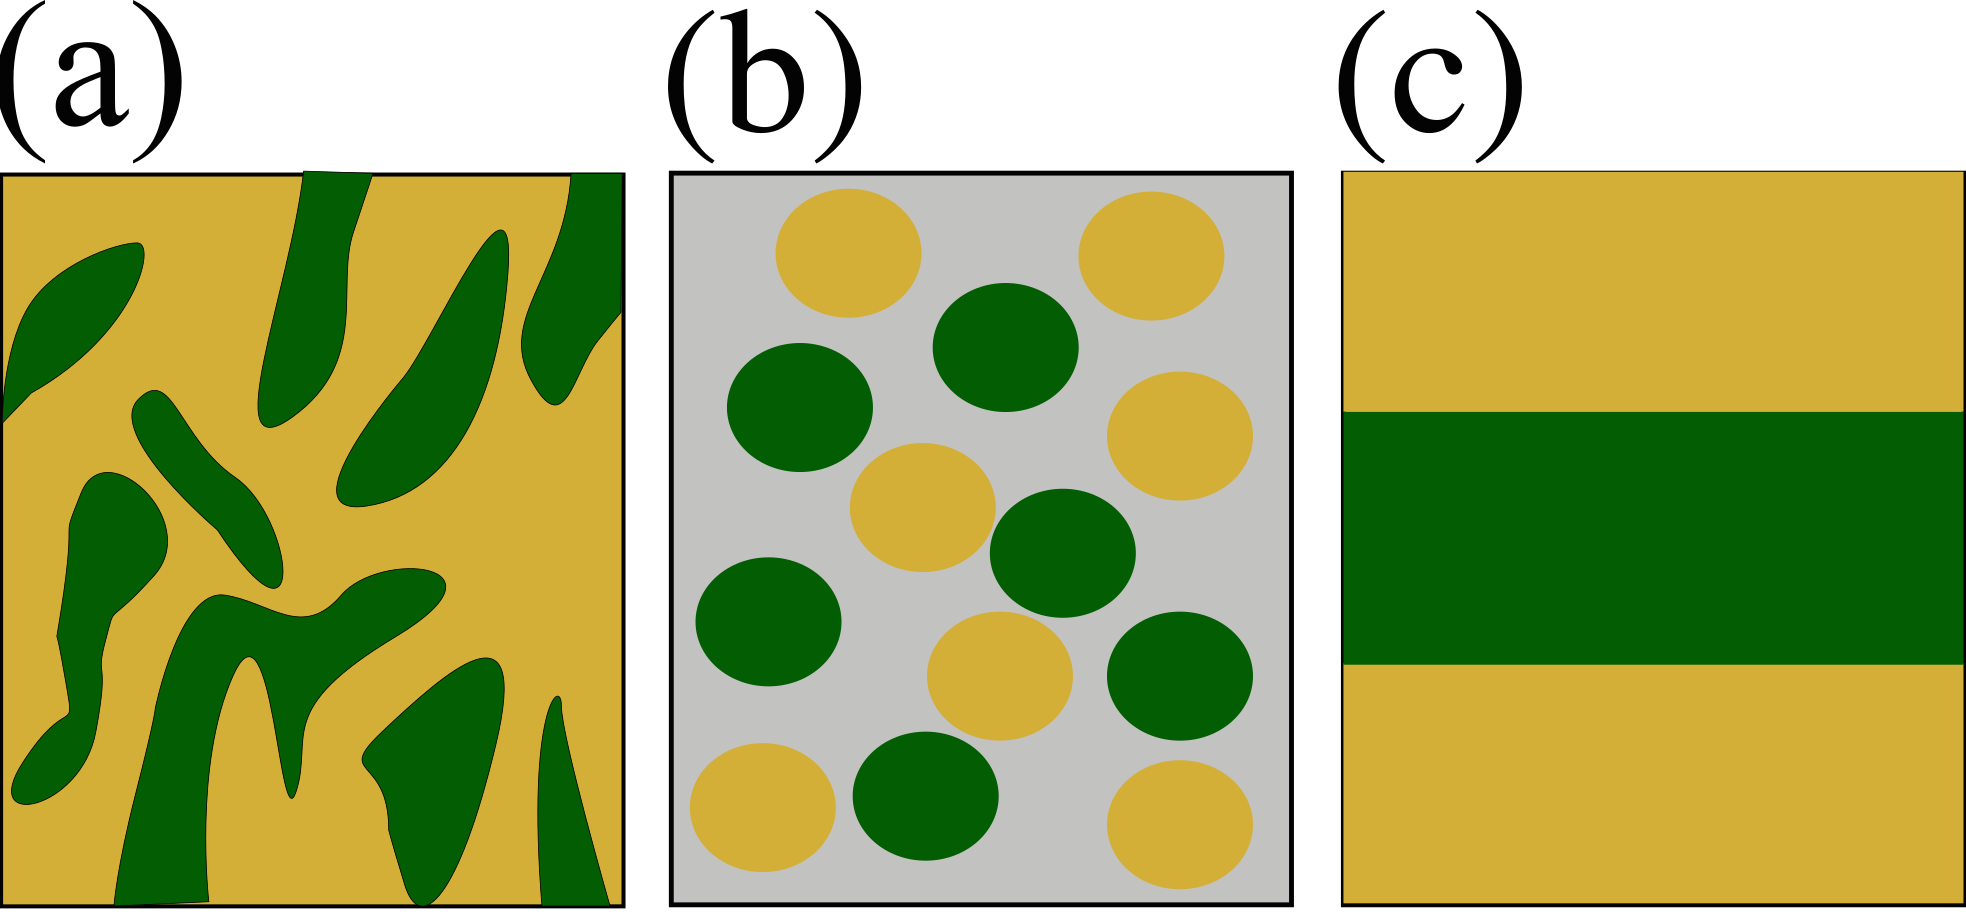
\includegraphics[scale=0.2]{hef/image1.png}
\end{figure}

\begin{figure}[h]
\caption{
Visualization of a 3-D Monte Carlo simulation of
electron transport in an Au-Fe-Au target heated by 7 keV photons,
incident normally from the top of the page. Electron tracks are
projected onto the plane of the page; showers resulting from
photoexcitation of Au and Fe atoms are red and blue, respectively. Note
that most of the electron tracks in the Fe are due to absorption events
in the Au.
}
\label{fig:hef_image2}
\centering
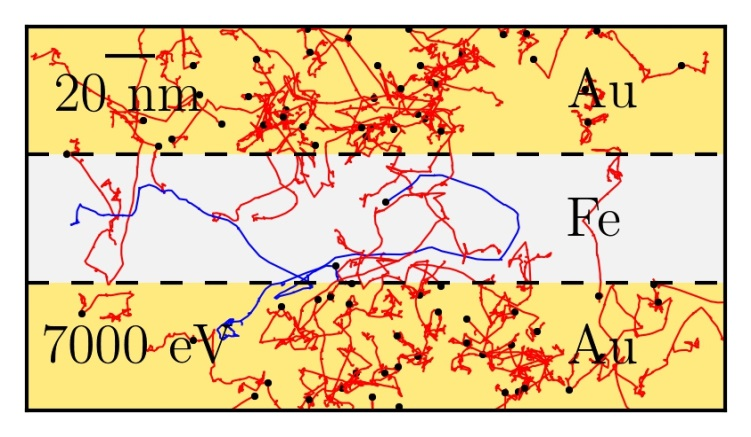
\includegraphics[scale=1.0]{hef/image2.jpeg}
\end{figure}

\begin{figure}[h]
\caption{
(a) Linear energy deposition density generated by 7 keV
photons incident on an Au-Fe\textsubscript{3}O\textsubscript{4}-Au
target, displayed for several thicknesses of the central
Fe\textsubscript{3}O\textsubscript{4} layer and a fixed Au cladding
thickness of 50nm. (b) Histograms of energy deposition density in volume
elements of the Fe\textsubscript{3}O\textsubscript{4} inclusions in
Au-Fe\textsubscript{3}O\textsubscript{4}-Au targets, displayed for
several thicknesses of the Au cladding and a fixed
Fe\textsubscript{3}O\textsubscript{4} layer thickness of 50 nm.
}
\label{fig:hef_image3}
\centering
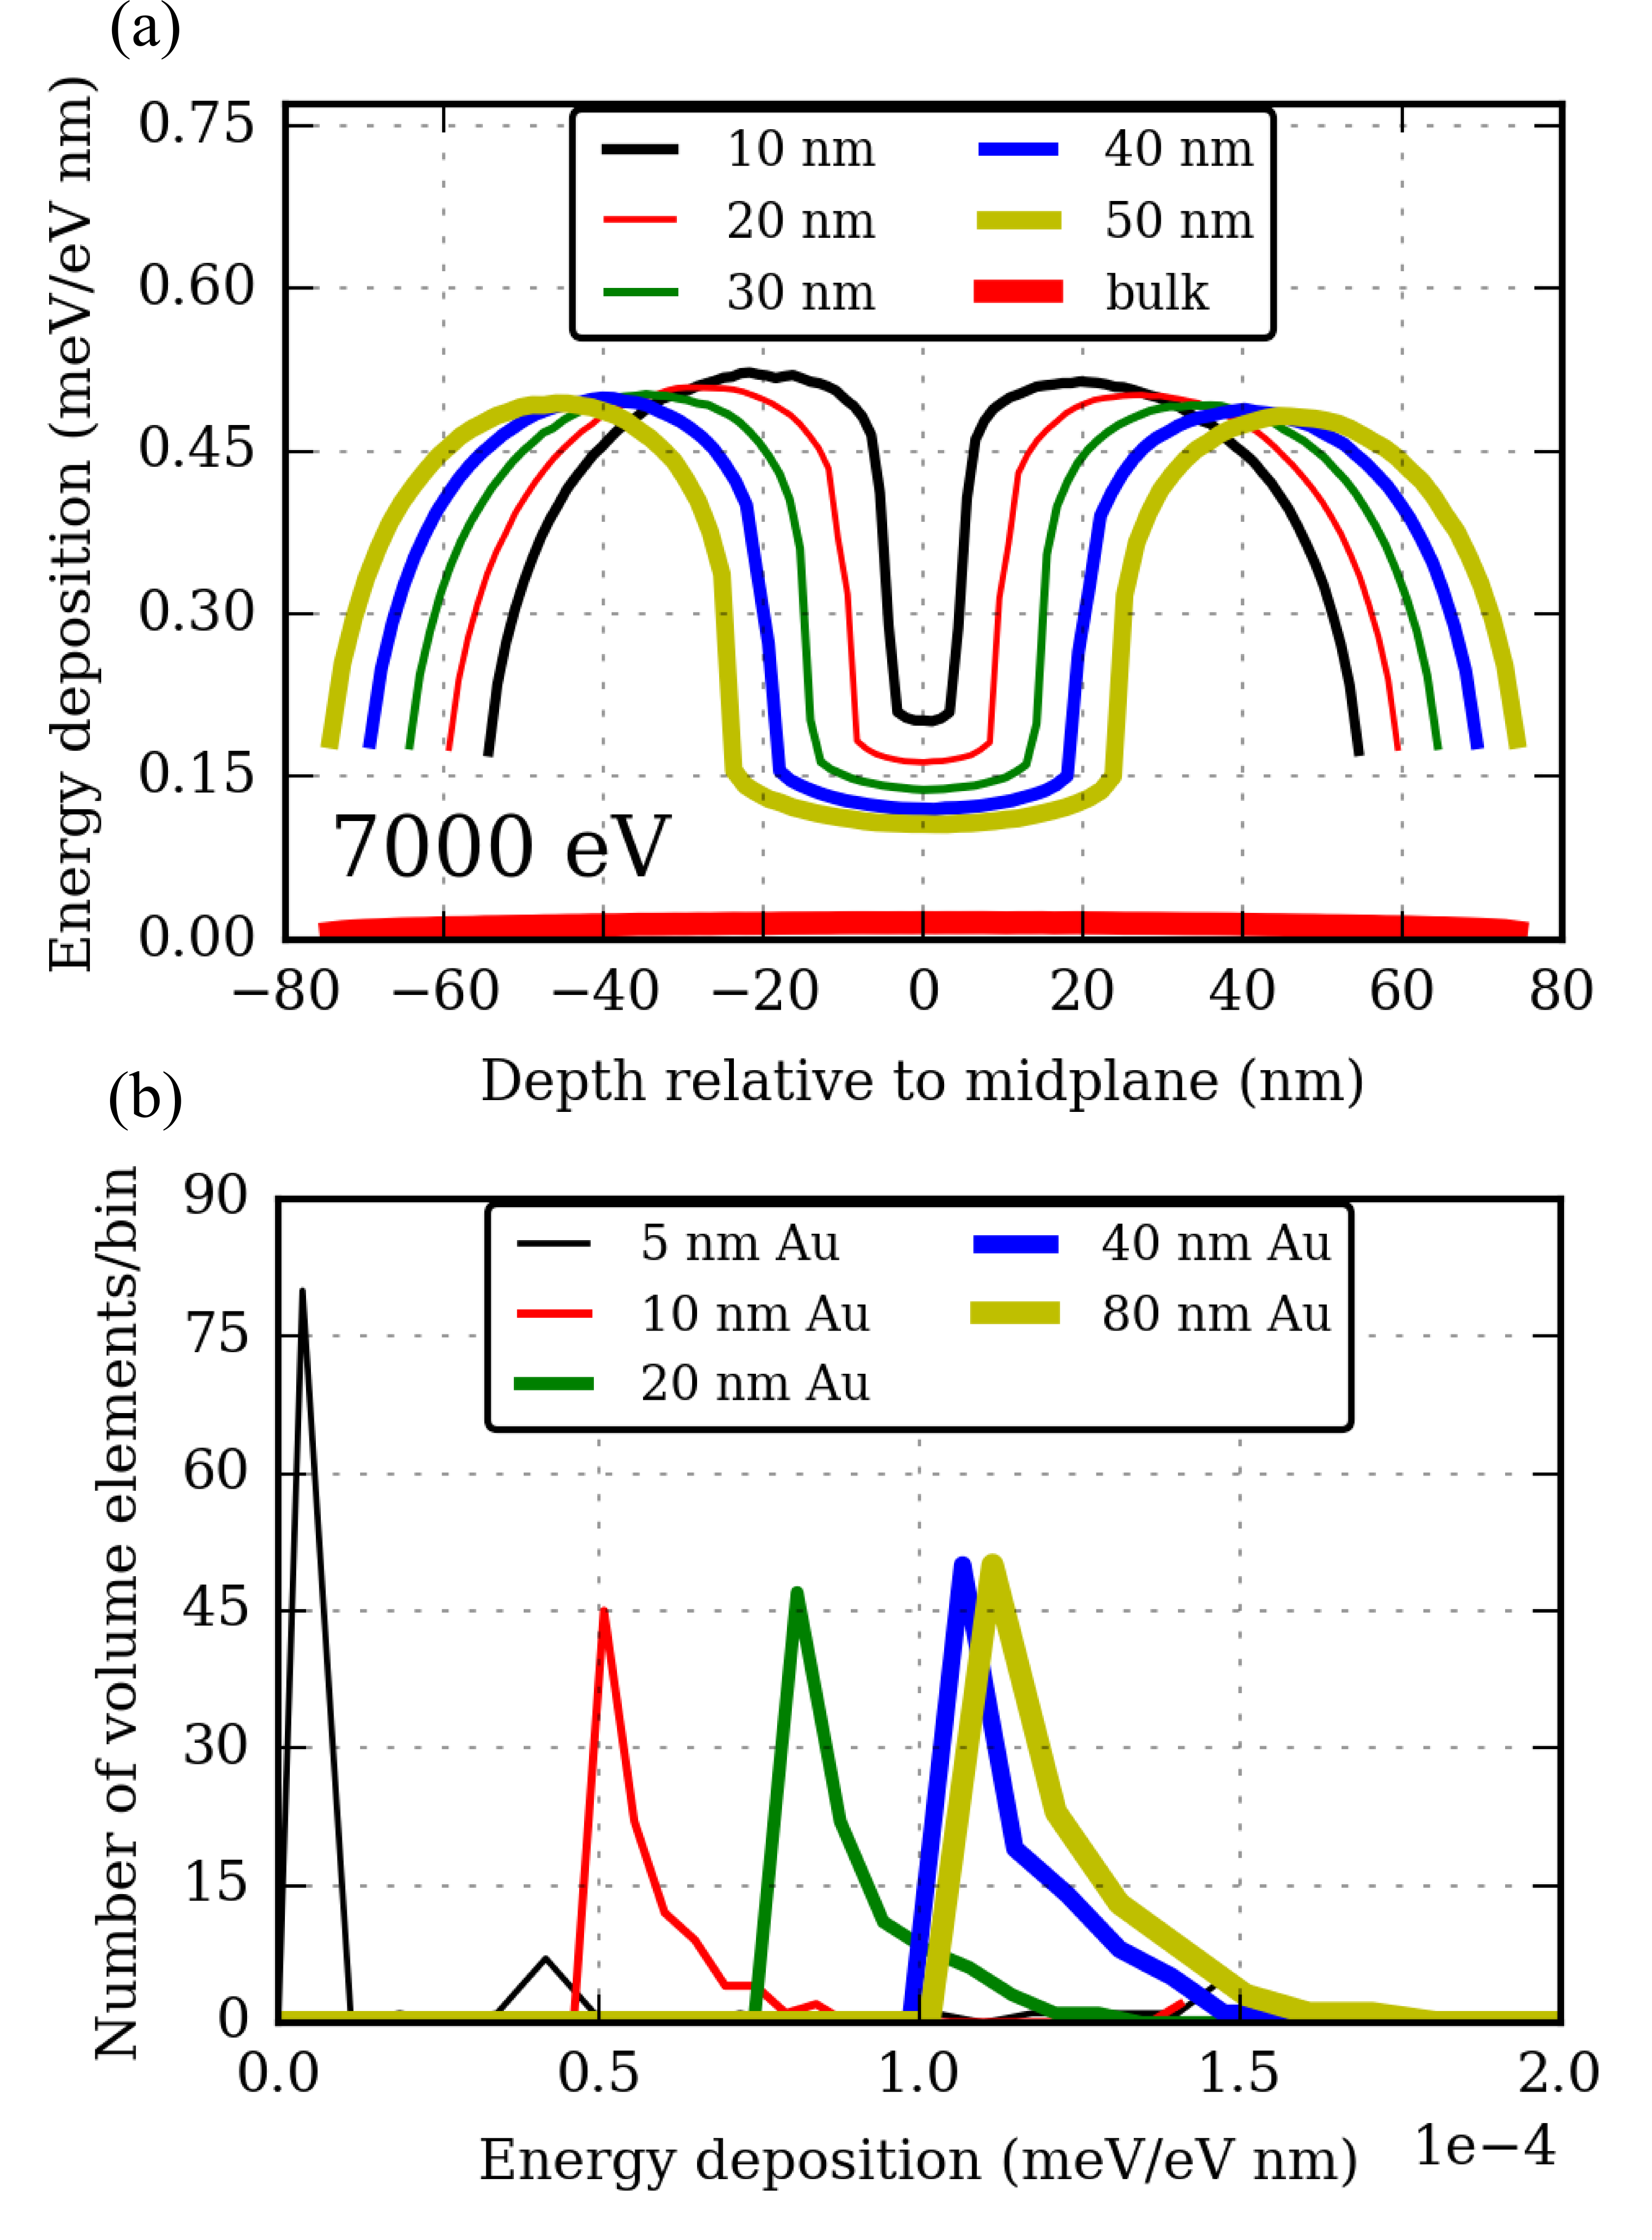
\includegraphics[scale=0.3]{hef/image3.png}
\end{figure}


\begin{figure}[h]
\caption{
%\hyperdef{}{OLEux5fLINK3}{}{\hyperdef{}{OLEux5fLINK4}{}{\hyperdef{}{OLEux5fLINK5}{}{}}}\textbf{4}.
Linear energy deposition due to 7 keV photons incident on an Au-C-Au
target displayed for several thicknesses of the central C layer and a
fixed outer cladding thickness of 50nm.
}
\label{fig:hef_image4}
\centering
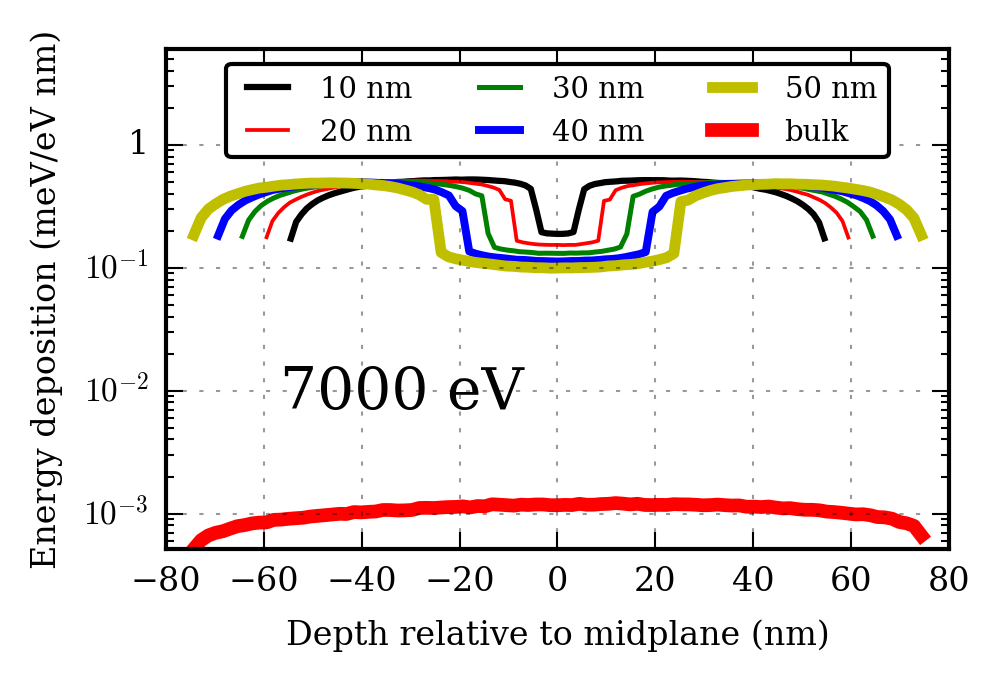
\includegraphics{hef/image4.png}
\end{figure}

\begin{figure}[h]
\caption{
%\hyperdef{}{OLEux5fLINK3}{}{\hyperdef{}{OLEux5fLINK4}{}{\hyperdef{}{OLEux5fLINK5}{}{}}}\textbf{4}.
Linear energy deposition in layered Au-Fe-Au and
Au-Fe\textsubscript{3}O\textsubscript{4}-Au targets of 150 nm total
thickness stimulated by 7 keV photons. Dashed lines indicate energy
deposition in bulk Fe\textsubscript{3}O\textsubscript{4} and Fe at
photon energies of 7.12 keV (above the iron K-edge) and 7 keV (below the
edge). The multilayer configuration sufficiently enhances energy
deposition so as to partially compensate for the difference between pre-
and above-edge x-ray photoelectric cross sections. The benefit is
particularly pronounced in Fe\textsubscript{3}O\textsubscript{4} due to
its much lower density and photoelectric cross-section.
}
\label{fig:hef_image5}
\centering
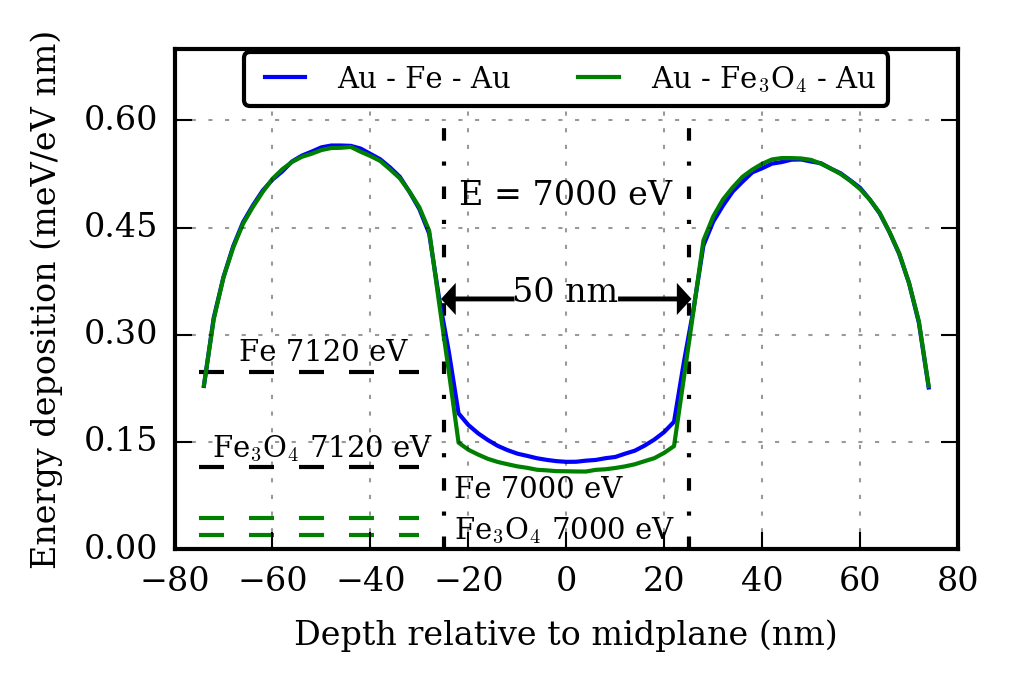
\includegraphics{hef/image5.png}
\end{figure}

\begin{figure}[h]
\caption{
Simulated powder diffraction of 50 nm Au-50 nm
Fe\textsubscript{3}O\textsubscript{4}-50 nm Au stimulated by X-rays
below the Fe K-edge (blue) compared to that resulting from photons above
the edge incident on bare Fe\textsubscript{3}O\textsubscript{4},
including fluorescence background(green).
}
\label{fig:hef_image6}
\centering
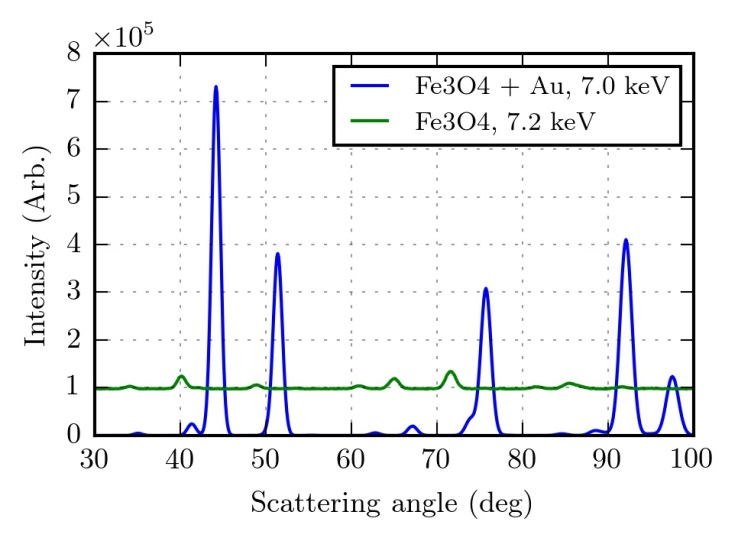
\includegraphics{hef/image6.jpeg}
\end{figure}





\chapter{A Photometric Study of Energy-Dispersive X-ray Diffraction at a Laser Plasma Facility}
\label{hef}

\begin{center}
O.R. Hoidn and G.T. Seidler\textsuperscript{(*)}

Physics Department

University of Washington

Seattle WA 98195-1560
\end{center}

\textbf{Abstract}

The low repetition rates and possible shot-to-shot variations in
laser-plasma studies place a high value on single-shot diagnostics. For
example, white-beam scattering methods based on broadband backlighter
x-ray sources are used to determine changes in the structure of
laser-shocked crystalline materials by the evolution of coincidences of
reciprocal lattice vectors and kinematically-allowed momentum transfers.
Here, we demonstrate that white-beam techniques can be extended to
strongly-disordered dense plasma and warm dense matter (WDM) systems
where reciprocal space is only weakly structured and spectroscopic
detection is consequently needed to determine the static structure
factor and thus the ion-ion radial distribution function. Specifically,
we report a photometric study of energy-dispersive diffraction (ED-XRD)
for structural measurement of high energy density systems at large-scale
laser facilities such as OMEGA and the National Ignition Facility. We
find that structural information can be obtained in single-shot ED-XRD
experiments using established backlighter and spectrometer technologies.

(*) Corresponding author:
\href{mailto:seidler@uw.edu}{\emph{seidler@uw.edu}}


\section{I Introduction}\label{i-introduction}

In addition to their centrality for inertial confinement fusion
studies,\hyperref[j.-d.-lindl-p.-amendt-r.-l.-berger-s.-g.-glendinning-s.-h.-glenzer-s.-w.-haan-r.-l.-kauffman-o.-l.-landen-and-l.-j.-suter-physics-of-plasmas-11-339-2004.]{\textsuperscript{1}}\textsuperscript{,}
\hyperref[e.-i.-moses-nuclear-fusion-49-104022-2009.]{\textsuperscript{2}}
laser-shock experiments play a growing role at the interface between
plasma physics and condensed matter physics, geosciences, and laboratory
astrophysics.\hyperref[f.-langenhorst-m.-boustie-a.-migault-and-j.-p.-romain-earth-and-planetary-science-letters-173-333-1999.]{\textsuperscript{3-14}}
However, for experiments reaching the highest energy density states the
technical challenges extend beyond the creation of such states: the low
repetition rates, limited facility access, and significant shot-to-shot
variations each place a special emphasis on single-shot x-ray
diagnostics of the structural and electronic properties of the
compressed, heated
target.\hyperref[b.-k.-f.-young-et-al.-review-of-scientific-instruments-69-4049-1998.]{\textsuperscript{15-24}}
An important case-in-point is provided by the determination of the
ion-ion radial distribution function,
\(g_{\text{ii}}\left( \overrightarrow{r} \right)\), or equivalently the
static structure factor \(S(\overrightarrow{k})\). Knowledge of
\(g_{\text{ii}}\left( \overrightarrow{r} \right)\) fulfills an
interesting variety of roles. First, it is necessary, if only at the
level of mean density and average ionization state, for investigation of
any equations of state (EOS) and of molecular dynamics simulations or
other structural calculations performed in support of EOS calculations.
Second, it is also a critical input parameter to any fine treatment of
electronic structure. The electronic structure of dense crystalline
systems and plasmas, in turn, is a quantity of fundamental interest but
also of a certain pragmatic interest: some sufficient knowledge of
electronic structure is needed for reliable determination of the target
temperature and ionization state in dense plasma and warm dense matter
(WDM) experiments
\hyperref[s.-h.-glenzer-and-r.-redmer-reviews-of-modern-physics-81-1625-2009.]{\textsuperscript{25}}\textsuperscript{,}
\hyperref[g.-gregori-et-al.-physics-of-plasmas-11-2754-2004.]{\textsuperscript{26}}\hyperref[s.-h.-glenzer-and-r.-redmer-reviews-of-modern-physics-81-1625-2009.]{},
and this capability is in turn needed for campaigns to experimentally
measure the EOS in the WDM regime
\hyperref[h.-j.-lee-et-al.-physical-review-letters-102-115001-2009.]{\textsuperscript{27-29}}.

For targets that retain substantial medium- or long-range order upon
shock compression, broadband backlighter x-ray sources enable white-beam
angle-dispersive x-ray diffraction (AD-XRD) in which substantial
structural detail can be inferred from Kossel rings
\hyperref[v.-lider-crystallography-reports-56-169-2011.]{\textsuperscript{30}}
and other fine scattering patterns dictated by the coincidence of
reciprocal lattice vectors and kinematically-allowed momentum transfers
\hyperref[m.-suggit-g.-kimminau-j.-hawreliak-b.-remington-n.-park-and-j.-wark-review-of-scientific-instruments-81-083902-2010.]{\textsuperscript{31}}\textsuperscript{,}
\hyperref[m.-j.-suggit-et-al.-nature-communications-3-1224-2012.]{\textsuperscript{32}}.
However, white-beam AD-XRD is only applicable to systems that are
substantially single crystalline: any statistically isotropic system,
whether a polycrystalline fine-powder sample or a dense, partially
ionized plasma, when illuminated by a broad-band source will show an
angularly-featureless signal when observed on, \emph{e.g}., an image
plate. For high atomic number (Z) systems, single-shot white-beam
extended x-ray absorption fine structure (EXAFS) has seen some
applications
\hyperref[b.-yaakobi-t.-r.-boehly-d.-d.-meyerhofer-t.-j.-b.-collins-b.-a.-remington-p.-g.-allen-s.-m.-pollaine-h.-e.-lorenzana-and-j.-h.-eggert-physical-review-letters-95-075501-2005.]{\textsuperscript{33}};
the situation has proven more challenging for lower-Z WDM and dense
plasmas, as a result of the mutually-exclusive target thickness
requirements of the x-ray measurement (soft x-ray penetration lengths of
order 1 micron or less) and laser ablation (necessary thicknesses of
tens of microns)
\hyperref[j.-l.-bourgade-et-al.-review-of-scientific-instruments-75-4204-2004.]{\textsuperscript{34}}.
Consequently, the first determination of
\(g_{\text{ii}}\left( r \right)\) for disordered, dense lower-Z plasma
systems
\hyperref[t.-ma-et-al.-physical-review-letters-110-065001-2013.]{\textsuperscript{35}}
instead used multi-shot, quasi-monochromatic AD-XRD, \emph{i.e.},
`traditional' XRD.

Here, we investigate whether single-shot, white-beam XRD can be
performed on \emph{strongly disordered}, laser-shocked solids and WDM
using spectral information at the detector location to parameterize the
momentum transfer of the quasielastic scattering event, \emph{i.e.,} we
consider purely energy-dispersive x-ray diffraction (ED-XRD). Some
context is needed to fully define this term and to distinguish it from
XRD methods already in use in the laser-plasma community. The
differential scattering cross section per atom for coherent scattering
of x rays (ordinary diffraction of incoherent incident photons) from an
isotropically disordered, elemental material such as a powder sample,
liquid, or dense laser-shock heated plasma of a single atomic species is

\(\frac{d\sigma_{\text{coh}}}{\text{dΩ}}\left( k \right) = \sigma_{t}S\left( k \right){f\left( k \right)}^{2}\)
(1)

where \(\sigma_{t}\) is the Thomson cross section, \(S(k)\) is the
directionally-averaged structure factor and \(f\left( k \right)\) is the
spherically averaged atomic form factor. The structure factor \(S(k)\)
is simply related by a sine transform to
\(g_{\text{ii}}\left( r \right)\),

\(S\left( k \right) = 1 + (4\ \pi\ \rho/k)\ \int_{0}^{\infty}{dr\ r\ \lbrack\ g_{\text{ii}}\left( r \right) - 1\rbrack}\ \sin{(kr})\).
(2)

These well\emph{-}known expressions establish the close connection
between XRD and \(g_{\text{ii}}\left( r \right)\) while also
demonstrating the need to measure the differential scattering
cross-section (and hence \(S(k)\)) at many different momentum transfers
if any significant constraint on the form of
\(g_{\text{ii}}\left( r \right)\) is to be obtained.

The \(k\)-dependence of \(d\sigma_{\text{coh}}/d\Omega\) can in
principle be measured with any suitable combinations of scattering angle
\(2\theta\) and photon energies spanning the needed momentum transfers:
\(k\) is chosen by the combined effect of these two
experimentally-selectable parameters,
\(k = \operatorname{(2E/c)sin}{2\theta}\). In practice, however, XRD is
measured in only two modes: angle-resolved XRD (henceforth `AR-XRD') and
energy-dispersive XRD (henceforth `ED-XRD'). Their distinction is best
introduced kinematically. As illustrated in Fig. \ref{fig:ed1}, any measurement of
\(S(k)\) must follow a curve in \(E\)-\(2\theta\) space which crosses
many of the shown contours of constant \emph{k.} The parameter space
probed by a typical AR-XRD experiment using $\sim 8$ keV
monochromatic incident photons is represented by the vertical curve in
the figure. Experimentally, the necessary apparatus will include a
monochromatic source and either an angle-scanning detector or a position
sensitive detector (PSD), which we show schematically in Fig. \ref{edimage2} (a) and
(b). On the other hand, a typical ED-XRD experiment instead resides on
the horizontal curve in Fig. \ref{fig:ed1}, \emph{i.e.}, at a fixed scattering angle
of 135 degrees but requiring both a broad incident source spectrum and
an energy-resolving detector. An experimental schematic for ED-XRD is
presented in Fig. \ref{edimage2}(c). We note that ED-XRD has a long history in
laboratory and synchrotron XRD studies, and plays an important role in
high-pressure diamond anvil cell research where the limited angular
access to the sample space substantially complicates
AD-XRD.\hyperref[y.-feng-m.-somayazulu-r.-jaramillo-t.-rosenbaum-e.-isaacs-j.-hu-and-h.-k.-mao-review-of-scientific-instruments-76-063913-2005.]{\textsuperscript{36-40}}
There is then an obvious commonality with experiments at large-scale
laser facilities; angular access at such facilities is strongly
constrained by the beam paths of the laser light itself.

AD-XRD from laser-shock compressed, disordered Al has recently been
reported by Ma, \emph{et
al.},\hyperref[t.-ma-et-al.-physical-review-letters-110-065001-2013.]{\textsuperscript{35}}
and this first such study illustrates both the scientific benefits and
technical drawbacks of AD-XRD for large-scale laser facilities.
Specifically, concerning the latter, a few high-resolution spectrometers
must be moved between different scattering angles for different shots so
as to obtain a complete characterization of \(S(k)\) by pooling the
results of many shots after suitable normalization or other
characterization of shot-to-shot variations in the source or target.
While the study of Ma, \emph{et
al.},\hyperref[t.-ma-et-al.-physical-review-letters-110-065001-2013.]{\textsuperscript{35}}
has overcome these challenges and provides an interesting comparison of
experiment to modern theoretical treatments of the structure of dense
plasmas, it is still important to note that the use of a multi-shot
technique has, at a minimum, decreased the range of phase space that can
be studied subject to the strong constraints that exist on facility
access. A single-shot alternative could therefore have high scientific
impact and is likely the only way that \(S(k)\) will be measured on
disordered dense plasmas at the National Ignition Facility, where the
number of shots per scientific study is especially limited.

Consequently, with the above context established, we report here a
photometric analysis of ED-XRD for laser-shock experiments illuminated
by broad-band backlighter sources. This analysis makes use of known
results for the spectrum of a broad-band backlighter, representative
experimental results for \(S(k)\) for disordered systems, and
representative, established technical characteristics of
spectrally-resolving detectors available at large-scale laser
facilities. We find significant benefits to ED-XRD for disordered
systems, including single-shot determination of \(S(k)\), and we propose
that ED-XRD should become a standard diagnostic at large-scale
facilities such as OMEGA and the National Ignition Facility

We continue as follows. In section 2 we describe the methods used in the
photometric analysis, including the reference target, modeled
experimental geometry, and any assumptions about detector or
spectrometer performance. In section 3 we present and discuss our
results for ED-XRD using each of two different experimental
configurations. These are, first, an x-ray CCD detector operating in
single-photon mode as an energy-resolving solid-state detector and,
second, a wavelength-dispersive spectrometer using a highly-oriented
pyrolytic graphite (HOPG) mosaic crystal as the diffractive element. The
CCD configuration is viable, but has some drawbacks associated with
saturation and double-counting that require special care. We find that
the HOPG-based spectrometer quite easily resolves the energy spectrum of
the diffraction with excellent counting statistics for a broad-band
backlighter that has been fielded at OMEGA, with the caveat that a
single HOPG crystal analyzer covers a narrower energy range, and hence a
more restricted \(k\)-range, than a CCD detector. Finally, in section IV
we conclude.

\section{II Methods}\label{ii-methods}

\subsection{II.A. Source and target}

One readily available broadband source in laser shock experiments is the
thermal spectrum from a laser-imploded polymer shell, usually filled
with H\textsubscript{2}-D\textsubscript{2} gas
\hyperref[b.-r.-maddox-et-al.-physics-of-plasmas-18-056709-2011.]{\textsuperscript{41}}\textsuperscript{,}
\hyperref[b.-yaakobi-f.-j.-marshall-t.-r.-boehly-r.-p.-j.-town-and-d.-d.-meyerhofer-journal-of-the-optical-society-of-america-b-optical-physics-20-238-2003.]{\textsuperscript{42}}.
In Fig. \ref{edimage3} we show a typical spectrum collected at OMEGA
\hyperref[b.-yaakobi-2012-private-communication.]{\textsuperscript{43}}.
Because of the spectrum's supra-exponential decay, an ED-XRD experiment
with this source is preferentially conducted at low energy, between 2
and 6 keV, as shown in the ED-XRD curve at a scattering angle of 135
degrees in Fig. \ref{fig:ed1}. Also shown in Fig. \ref{edimage3} is the spectrum for a typical
narrow band backlighter source at OMEGA, where these sources have seen
extensive use in x-ray scattering studies, both elastic (XRD)
\hyperref[t.-ma-et-al.-physical-review-letters-110-065001-2013.]{\textsuperscript{35}}
and inelastic (usually called `x-ray Thomson scattering')
\hyperref[s.-h.-glenzer-and-r.-redmer-reviews-of-modern-physics-81-1625-2009.]{\textsuperscript{25}}.
The narrow-band spectrum is obtained by scaling the spectrum of a Cu
\emph{K\textsubscript{α}} target driven by a 10 J, 10 ps laser pulse at
the MTW laser facility to a 2.5 kJ, 10 ps laser pulse at OMEGA, using a
typical \emph{K\textsubscript{α}} photon yield of 4 ×
10\textsuperscript{10} photons per J of laser energy
\hyperref[p.-m.-nilson-2012-private-communication.]{\textsuperscript{44}}\textsuperscript{,}
\hyperref[k.-u.-akli-et-al.-physics-of-plasmas-14-023102-2007.]{\textsuperscript{45}}.

\begin{figure}[h]
\caption{
Contours of equal momentum transfer \(k\) (labeled in units of
Å\textsuperscript{-1}) in energy and scattering angle. Angle-dispersive
x-ray diffraction (AD-XRD) and energy-dispersive x-ray diffraction
(ED-XRD) take vertical and horizontal cuts, respectively, to achieve
broad coverage in \(k\) and thus obtain information about the radial
distribution function.
}
\label{fig:ed1}
\centering
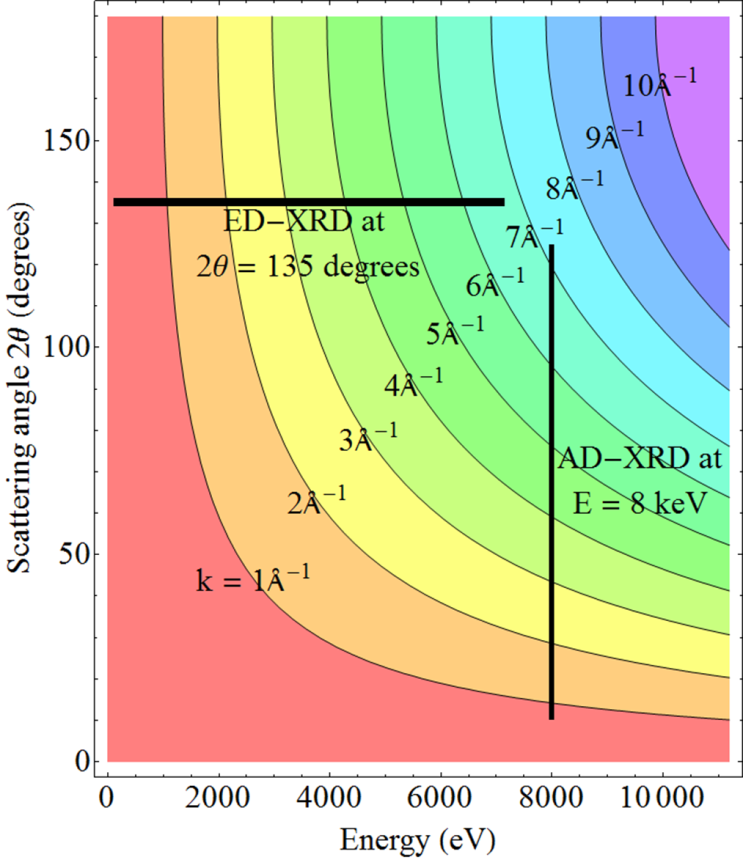
\includegraphics{media/image1.png}
\end{figure}

We consider two target systems where experimental \(S(k)\) are
available: liquid boron at ambient pressure and shock-compressed
aluminum. For liquid boron we use the experimental results of Krishnan
\emph{et al.}
\hyperref[s.-krishnan-s.-ansell-j.-j.-felten-k.-j.-volin-and-d.-l.-price-physical-review-letters-81-586-1998.]{\textsuperscript{46}}\textsuperscript{,}
\hyperref[s.-krishnan-and-d.-l.-price-journal-of-physics-condensed-matter-12-r145-2000.]{\textsuperscript{47}},
the data for which were taken at a synchrotron light source using
hydrodynamically-levitated boron heated to 2400K by continuous
illumination from infrared lasers. While this is not a WDM system
\emph{per se}, it is a reasonable surrogate. As shown in Fig. \ref{edimage4} (a),
note the presence of a few broad peaks in \(S(k)\), representative of a
system with only limited, short-range information in
\(g_{\text{ii}}\left( r \right)\). For clarity in our photometric
analysis, we will use a smoothed \(S(k)\) where the sharp (nonphysical)
noise in the experimental \(S(k)\) has been filtered. On the other hand,
\(S(k)\) for shock-compressed aluminum (\(n_{e}\)= 5.4 ×
10\textsuperscript{23} cm\textsuperscript{-3}; \(T_{e}\)= 10 eV) is
based on results from Ma \emph{et
al.}\hyperref[t.-ma-et-al.-physical-review-letters-110-065001-2013.]{\textsuperscript{35}},
who have recently reported the first AD-XRD measurement of a
shock-compressed, disordered WDM system. \(S(k)\) was recovered from Ma
\emph{et al.}'s theoretical calculation of an elastic scattering profile
for triply-ionized shock-compressed aluminum, to which they fit their
data. We note that only an approximate atomic form factor, that of
ambient aluminum, was used to calculate \(S(k)\) from the scattering
profile; however, the resulting error in \(S(k)\) is expected to be
negligible above \(k = 3A^{- 1}\), and hence does not affect the
location of any coordination peaks. As shown in Fig. \ref{edimage4} (b), note again
that the presence of only short-range order in the target results in a
simple form for \(S(k)\). In this case, the information content is
largely limited to the location and intensity of the obvious first
coordination peak.


\begin{figure}[h] \label{edimage4}
\caption{ (a): Liquid structure factor of B at 2400K. The original data
(red) of Krishnan \emph{et al.}
\hyperref[s.-krishnan-s.-ansell-j.-j.-felten-k.-j.-volin-and-d.-l.-price-physical-review-letters-81-586-1998.]{\textsuperscript{46}}
contains sharp unphysical noise; we therefore use the filtered
interpolation (blue) of the data for \(S(k)\) throughout this paper.
(b): Equivalent theoretical curve for shock-compressed Al at electron
density \(n_{e}\) = 5.4 × 10\textsuperscript{23} cm\textsuperscript{-3}
and temperature \(T_{e}\) = 10 eV based on Ma \emph{et al.}
\hyperref[t.-ma-et-al.-physical-review-letters-110-065001-2013.]{\textsuperscript{35}}
The curve is based on an approximate treatment of this system's atomic
form factor (see the text for details).}
\centering
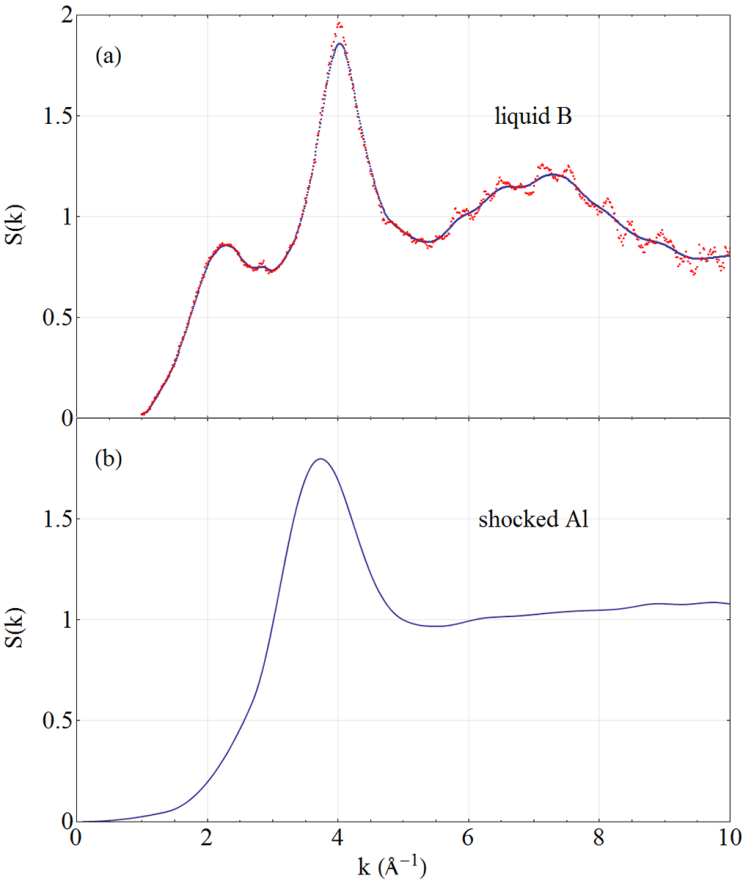
\includegraphics[scale=1.0]{media/image4.png}
\end{figure}

\subsection{II.B. Photon-electron interactions and numerical modeling }

For the targets considered here, the experiment is conducted in an
energy region far above any atomic fluorescence from the targets and
also far above any soft x-ray blackbody radiation from the surface or
bulk of the target, each of which is easily attenuated in practice with
a thin plastic or Be shield. Consequently, we need only consider the
coherent and incoherent scattering of the x-rays as direct contributors
to the measured scattering signal; the photoelectric interaction appears
only in its contribution to absorption coefficient in the energy range
of interest. Note that by coherent here we refer to the quasielastic
scattering process itself, \emph{i.e.} ``ordinary'' diffraction, with no
expectation of coherence of the incident beam (such as is used in
diffraction experiments at XFEL facilities).

Given a backlighter source with fluence
\(I_{\text{source}}\left( E \right)\) (units of photons/eV, integrated
over 4π steradian) at a distance \(d_{\text{sour}\text{ce}}\) from the
target, the areal flux incident in the target is
\(I_{\text{incident}}\left( E \right) = I_{\text{source}}\left( E \right)/4\pi d_{\text{source}}^{2}\).
The contribution of coherent scattering to the measured energy spectrum
at a scattering angle \(2\theta\) is then

\(I_{\text{coh}}\left( E,2\theta \right) = I_{\text{incident}}\left( E \right)\ \frac{d\sigma_{\text{coh}}}{\text{dΩ}}\left( k \right)\text{\ d}\Omega_{\det}\ \eta_{\det}\left( E \right)\ \tau_{\text{coh}}\left( E,2\theta \right)\),
(3)

where \(k\) is implicitly determined by \(E\) and \(2\theta\) ,
\(d\Omega_{\det}\) is the solid angle subtended by the detector,
\(\eta_{\det}\left( E \right)\) is the net efficiency of detection of
photons of energy \(E\) that arrive in \(d\Omega_{\det}\), and
\(\tau_{\text{coh}}\left( E,2\theta \right)\) includes the necessary
corrections to the measured XRD due to the target's geometry and
energy-dependent absorption coefficient
\hyperref[j.-l.-bourgade-et-al.-review-of-scientific-instruments-75-4204-2004.]{\textsuperscript{34}}.
When operating near to a backscattering geometry, for example,
\(\tau_{\text{sample}}\left( E,2\theta \right)\ \ \sim\ \rho\ A(1 - \ e^{- 2\ \mu\left( E \right)d})/2\ \mu(E)\ \)where
\(\rho\) is atomic (number) density, \(A\) is the cross-sectional area
of the portion of the backlighter beam that illuminates the target
region of interest, \(d\) is the target thickness, and
\(\mu\left( E \right)\) is the x-ray absorption coefficient. For present
purposes, \(d\sigma_{\text{coh}}/d\Omega\) includes all elastic and
quasielastic scattering; it integrates over all ion-ion correlation
dynamics
\hyperref[g.-gregori-and-d.-o.-gericke-physics-of-plasmas-16-056306-2009.]{\textsuperscript{48}}.

The incoherent contribution to the measured signal is somewhat more
complex to model. The microscopic physics of the incoherent scattering
processes, wherein one must address both momentum transfer (\(k\)) and
energy transfer (\(\text{ℏω}\)), results in the need for a double
differential cross-section
\(d^{2}\sigma_{\text{incoh}}\frac{\left( k,\omega \right)}{\text{dωd}}\Omega\).
The detected intensity from incoherent scattering is then

\(I_{\text{incoh}}\left( E,\ 2\theta \right) = d\Omega_{\det}N_{\text{atoms}}\ \frac{d\sigma_{t}}{d\Omega}\int_{0}^{\infty}{dE'I_{\text{incident}}\left( E' \right)}\ S_{\text{incoh}}\left( k,\ \omega \right)\tau_{\text{incoh}}\left( E^{'},E,2\theta \right)\)
(4),

where \(N_{\text{atoms}}\) is the number of atoms in the target, \(k\)
is again implicitly determined by \(E\), \(E'\)\emph{,} and \(2\theta\)
and \(\tau_{\text{incoh}}\left( E^{'},E,2\theta \right)\) includes the
influence of attenuation for an incident photon of energy \(E'\) that
scatters through an angle \(2\theta\) and departs the incoherent
interaction with energy \(E\). In the first Born approximation,
\(d^{2}\sigma_{\text{incoh}}/d\omega d\Omega = (d\sigma_{t}/d\Omega)\ S_{\text{incoh}}\left( k,\ \omega \right),\)
where \(d\sigma_{t}/d\Omega\) is the Thomson differential scattering
cross section and \(S_{\text{incoh}}\left( k,\ \omega \right)\) is the
inelastic component of the dynamic structure factor. In the
independent-electron approximation
\hyperref[j.-chihara-journal-of-physics-condensed-matter-12-231-2000.]{\textsuperscript{49}}\textsuperscript{,}
\hyperref[w.-schuelke-electron-dynamics-by-inelastic-x-ray-scattering-oxford-university-press-new-york-2007.]{\textsuperscript{50}},
\(S_{\text{incoh}}\left( k,\ \omega \right)\) may be expressed as a sum
over electrons and matrix elements between the initial and final states
of the system:

\(S_{\text{incoh}}\left( k,\ \omega \right) = \ \sum_{j}^{}{\sum_{f \neq i}^{}{\left| \left\langle {i|e}^{\text{i\ }\mathbf{q \bullet}\mathbf{r}_{\mathbf{j}}}|f \right\rangle \right|^{2}\delta(E_{f} - \ E_{i} - \ \omega)}}\).
(5)

At sufficiently high
\(k\),\(\ S_{\text{incoh}}\left( k,\ \omega \right)\) is peaked at the
Compton shift \(\Delta E = \hbar^{2}k^{2}/2\ m\). In the high\emph{-}\(k\)
(non-collective) scattering regime the total inelastic portion of the
dynamic structure factor is constructed using equation (5) evaluated as
a sum over individual valence and core electrons. In our modeling
procedure this consists of truncated valence and core Compton profiles
generated in the impulse approximation
\hyperref[w.-schuelke-electron-dynamics-by-inelastic-x-ray-scattering-oxford-university-press-new-york-2007.]{\textsuperscript{50}}\textsuperscript{,}
\hyperref[p.-eisenberger-and-p.-m.-platzman-physical-review-a-2-415-1970.]{\textsuperscript{51}}
where \(S_{\text{incoh}}\left( k,\ \omega \right)\) depends only on the
ground state electronic density and kinematics of the scattering
process. The first moment of
\(\ S_{\text{incoh}}\left( k,\omega \right)\) was normalized after
truncation according to the Bethe \emph{f}-sum rule
\hyperref[b.-a.-mattern-g.-t.-seidler-j.-j.-kas-j.-i.-pacold-and-j.-j.-rehr-physical-review-b-85-115135-2012.]{\textsuperscript{52}}.
For boron our approximation yields incoherent scattering cross sections
which exceed experimental values by up to 30 percent, making our
approximate treatment of the incoherent background conservative. In the
relevant range of momentum transfers the Compton shift is sufficiently
small that we substitute \(\tau_{\text{coh}}\left( E,2\theta \right)\)
for \(\tau_{\text{incoh}}\left( E,\ E',2\theta \right)\) without
introducing appreciable systematic error, allowing \(\tau\) to be
factored out of the integrand in equation (4). Similarly, the FWHM of
\(\ S_{\text{incoh}}\left( k,\ \omega \right)\) (which, in the impulse
approximation, is directly related to the width of the momentum
distribution of the electronic ground state) is small compared to our
required energy resolution, such that we can define a Compton-shifted
energy variable \(E^{*} = E + \ \Delta E\) and re-express (4) in
approximate form:

\(I_{\text{incoh}}\left( E,2\theta \right) = d\Omega_{\det}N_{\text{atoms}}\text{\ \ }\frac{d\sigma_{t}}{d\Omega}\ \tau_{\text{coh}}\left( E,2\theta \right)\ I_{\text{incident}}\left( E^{*} \right)\int_{0}^{\infty}{dE'}\text{\ \ }S_{\text{incoh}}\left( k,\ \omega \right)\).
(6)

The total scattered intensity, in units of photons/sr, is then

\begin{equation}
\begin{aligned}
I_{total}(E) = &~d\Omega_{t} N_{atoms} \tau(E, 2\theta) \frac{d\sigma_t}{d\Omega} [I_{Iincident}(E) f(k)^2 S(k) +\\
& I_{incident}(E) \int_0^\infty dE' S_{incoh}(k, \omega)].
\end{aligned}
\end{equation}

Note that
\(\int_{0}^{\infty}{dE'}\ S_{\text{incoh}}\left( k,\ \omega \right) = N\)
(the atomic number of the scattering species) in the high\emph{-}\(k\)
limit of the impulse
approximation\hyperref[p.-eisenberger-and-p.-m.-platzman-physical-review-a-2-415-1970.]{\textsuperscript{51}}
and takes on smaller values at lower momentum transfers; by comparison,
\({f(0)}^{2} = N^{2}\), and \(S(k)\) is of order unity. Therefore the
first (coherent) term in \(I_{\text{total}}\left( E \right)\) dominates
for heavier elements or for sufficiently small momentum transfers. In
Fig. \ref{edimage5} (a) and (b) we compare \({f(k)}^{2}\) to the incoherent
background scattering for the above-described model. These results lead
us to expect that the background in an ED-XRD experiment will not
substantially limit the ability to observe the desired coherent
scattering.

\subsection{II.C. Spectrometers for detection of ED-XRD}

We now consider two different detection options. As shown in the
schematic of Fig. \ref{edimage2}, one or both of an x-ray CCD and a HOPG-based
spectrometer may be used as energy-sensitive detectors. Simulated
spectra for both follow in section III. Throughout the remainder of the
paper the following experimental parameters are used:
\(d_{\text{source}}\) = 1 cm; target dimensions (for both B and Al):
0.25 mm × 0.25 mm × 0.1 mm; scattering angle \(2\theta\) = 135 degrees.
These choices will be motivated below.

\begin{figure}[h] 
\caption{ Schematic representations of (a) and (b) angle-dispersive
x-ray diffraction, compared to (c) energy-dispersive x-ray diffraction
(ED-XRD).}
\label{edimage2}
\centering
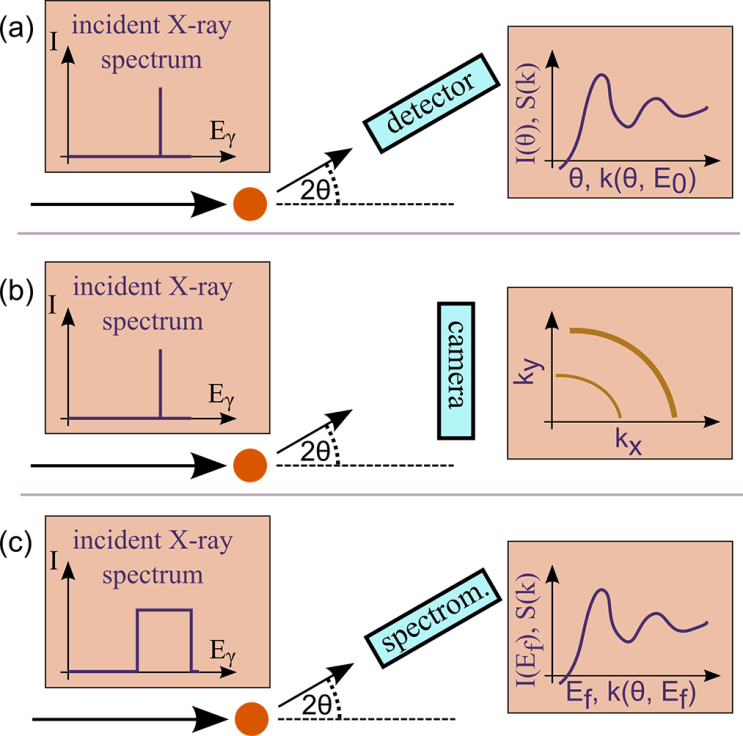
\includegraphics[scale=1.0]{media/image2.png}
\end{figure}

The modeled CCD has a 2-dimensional square grid of 2200 x 2200 pixels,
with a pixel edge length of 13.5 microns. A quantum efficiency of 1 is
assumed. The optimal distance between the detector and the target is
determined by the competing demands of high signal collection and high
rejection of two-photon events on single pixels. We find it reasonable
to balance these demands by selecting a single photon-hit regime with an
expectation value \(p\) of 0.1 photon hits per pixel. At a given
scattering angle and in the absence of addition of any special absorbers
between the target and the CCD other than a Be filter for low-energy
photon rejection, \(p\) is determined by the working distance of the CCD
and the scattered intensity off the target. The working distance is not
a highly-constrained parameter; it must merely be sufficiently large
that backgrounds from the high neutron flux and other stray radiations
are likely to be substantially suppressed. An upper bound on target
intensity arises from signal broadening due to the finite angular size
subtended by the target relative to the backlighter. We require this
geometrical broadening in momentum transfer, \(\text{Δk}\)\emph{,} to
satisfy \(\Delta k/k\ \  < \ 0.05\), such that it is sufficiently small
compared to the intrinsic scale of structure in \(S(k)\). We label the
angle subtended by the target \(\Delta\theta_{t}\) and express the
geometrical broadening in terms of it:
\(\Delta k/k\  = \ \cot{\text{θ\ Δ}\theta_{t}}.\) At
\(2\theta\  = \ 135\ degrees\) the maximal \(\Delta\theta_{t}\) is
approximately 0.1 radians, which corresponds to a sample length of 1 mm.

The task of presenting a modeled HOPG spectrum in a
non-configuration-specific manner is complicated by the significant
dependence of the spectrometer's energy range on several geometric
parameters. Using the labeling of Fig. \ref{edimage6} and, as an example, the
spectrometer geometry described by Fig. \ref{edimage7} (a), the differential in \(k\)
for scattering from the target is

\begin{figure}[h] 
\caption{ Experimental configuration
for ED-XRD at a laser shock facility. A long pulse-driven CH capsule
emits a broad thermal spectrum. Scattering from the target is observed
using an HOPG spectrometer or a CCD in the single-photon hit regime.}
\label{edimage6}
\centering
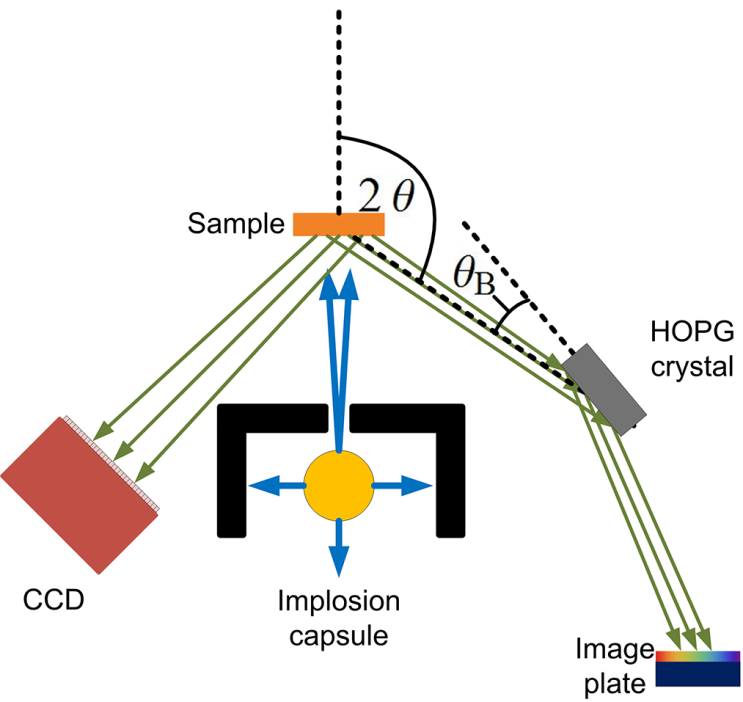
\includegraphics[scale=1.0]{media/image6.png}
\end{figure}

\(dk = \ \frac{\text{δk}}{\text{δE}}\ dE + \ \frac{\text{δk}}{\delta(2\theta)}\ d(2\theta) = \ \frac{E}{\text{ℏc}}\left( \sin{(\theta)\ \cot{\theta_{B}\  - \ \cos{(\theta)}}}\  \right)\text{dθ}_{B}\).
(9)

As a crystal of length \(l\) located a distance \(F\) from the target
subtends an angle of approximately (\(l/F)\ \sin\theta_{B}\), we can
directly use (9) to calculate the range \(\text{Δk}\) covered by an
analyzer crystal as a function of \(k\)\emph{,}\(\ 2\theta,\) and the
choice of HOPG reflection. Fig. \ref{edimage7} illustrates this. Salient features of
\(\Delta k(k,\ 2\theta)\) are that it is asymptotically linear in \(k\)
and depends weakly on \(2\theta\ \)everywhere except at low
\(k\)\emph{.}

\begin{figure}[h] 
\caption{ Range Δ\emph{k} in momentum transfer of scattering off the
target probed by a small HOPG crystal per degree of its maximum
subtended angle, \(\theta_{\max}\), for three spectrometer geometries
that involve the same position (but different rotations) of the HOPG
crystal: (a) the detector located in the target scattering plane and
away from the axis passing through the backlighter and target, (b) the
detector located in the target scattering plane and near the axis
passing through the backlighter and target, and (c) the detector located
such that it, the target, and the HOPG crystal define a plane
perpendicular to the scattering plane. θ\textsubscript{max} denotes the
maximum possible subtended angle of the HOPG crystal given a fixed
spectrometer working distance \(F\); \emph{i.e.}, for a crystal of
length \(l\), the maximum subtended angle is
\(\theta_{\max} = \ l/F\)\emph{.}}
\label{edimage7}
%\hyperdef{}{ux5fRef350527476}{}{}
\centering
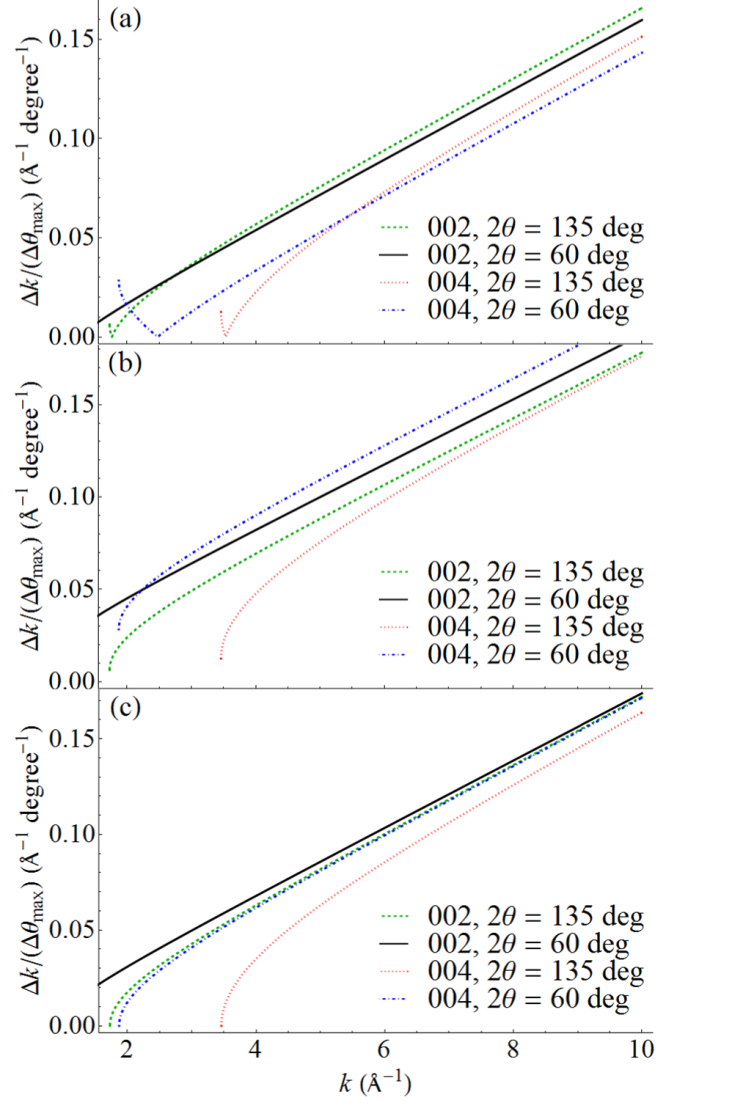
\includegraphics[scale=1.0]{media/image7.png}
\end{figure}

That said, we can choose a typical configuration for an HOPG
spectrometer and generate a detected spectrum that spans the entire
range of \(k\) with which we are concerned. Conceptually, this is done
by repeatedly rotating the crystal to different central \(\theta_{B}\)
to acquire narrow spectra in different ranges of \(k\) and then
stitching together the resulting spectra. This spectrum, which is
henceforth referred to as the ``HOPG source spectrum'', does not
represent a realistic data set, since acquiring it in a single shot
would require prohibitively many analyzer crystals, but it does serve as
a convenient compilation of the ensemble of possible experimental
configurations; the exact choice of spectrometer configuration for a
given experiment depends on some prior knowledge of the desired \(k\)
range, as we discuss below.

The modeled HOPG spectrometer is qualitatively similar to several
instruments that have previously been fielded for x-ray Thomson
scattering studies at OMEGA \textsuperscript{53-55}. For our modeled
instrument, the HOPG diffractive element operates on the 002 reflection,
has a mosaic spread of 0.3 degrees, is taken to be a flat square with
side length \(l\) = 12 cm, and is located at a distance \(F\) \emph{=}
25 cm from the target. The energy-dependent integral reflectivity of the
HOPG is based on computed reflectivity curves
\hyperref[a.-k.-freund-a.-munkholm-and-s.-brennan-optics-for-high-brightness-synchrotron-radiation-beamlines-ii-2856-68-1996.]{\textsuperscript{56}}
for an HOPG crystal having a mosaic spread of 0.3 degrees. Denoting
\(r\) as the peak reflectivity and \(\omega\) as the FWHM of the
reflectivity curve, the angular integral reflectivity,
\(\Delta\theta_{B},\) is approximately \(\text{rω}\)\emph{;}
equivalently, the integral reflectivity in energy units is
\(\Delta E = E\cot{\theta_{B}\Delta\theta_{B}}\). We define \(E_{\max}\)
and \(E_{\min}\) as the maximum and minimum energies diffracted by the
crystal. For isotropically-scattered photons with a fixed energy \(E\)
between \(E_{\max}\) and \(E_{\min}\) the probability of reflection is
\(\eta\  = \ \Omega_{0}\Delta E/(4\ \pi\ \left( E_{\max} - \ E_{\min} \right))\),
where \(\Omega_{0} = ({l/F)}^{2}\ \sin\theta_{B}\) is the solid angle
subtended by the crystal relative to the source (units of sr).
Correspondingly, the detected spectrum resulting from
\(I_{\text{incident}}\) on the target is
\(I_{d}\left( E \right) = 4\pi\eta dI_{\text{incident}}\left( E \right)/d\Omega = \Delta\theta_{B}(l/F)dI_{\text{incident}}\left( E \right)/d\Omega\).
For reference, \(\Delta\theta_{B}l/F = 7 \times 10^{- 4}\) at 4 keV. It
will be seen in the next section that the resulting net collection
efficiency in a given achievable energy band is several orders of
magnitude higher than that of the CCD.

\section{III Results and
discussion}\label{iii-results-and-discussion}

There is good reason to believe, heuristically, that the above-described
experimental configurations for ED-XRD should determine
\(S\left( k \right)\) with adequate statistics. Numerous past x-ray
Thomson scattering experiments at laser plasma facilities have measured
the inelastic portion of \(S\left( k,\omega \right)\) using narrow pulse
backlighters for illumination
\hyperref[s.-h.-glenzer-and-r.-redmer-reviews-of-modern-physics-81-1625-2009.]{\textsuperscript{25}}\textsuperscript{,}
\hyperref[h.-j.-lee-et-al.-physical-review-letters-102-115001-2009.]{\textsuperscript{27}}\textsuperscript{,}
\hyperref[c.-fortmann-h.-j.-lee-t.-doeppner-r.-w.-falcone-a.-l.-kritcher-o.-l.-landen-and-s.-h.-glenzer-physical-review-letters-108-175006-2012.]{\textsuperscript{28}}\textsuperscript{,}
\hyperref[r.-tommasini-et-al.-review-of-scientific-instruments-79-10e901-2008.]{\textsuperscript{57-60}}.
Above 2 keV, a broad-band thermal backlighter has approximately 100
times the photon conversion efficiency of a short-pulse Cu
\emph{K\textsubscript{α}} backlighter (Fig. \ref{edimage3}); additionally, the
elastic scattering cross section is typically larger than the Compton
cross section, as discussed in section II and shown in Fig. \ref{edimage5} (a) and 5
(b). Thus, ED-XRD should offer vastly higher signal intensity than
(quasi-monochromatic) x-ray Thomson scattering using a metal-foil
backlighter, and therefore better statistics.

\begin{figure}[!ht] 
\caption{ Elastic and inelastic contributions to the differential cross
section of (a) boron and (b) aluminum. The elastic cross sections are
based on tabulated values of \(f(k)\). The inelastic differential cross
sections, defined by
\(N_{\text{incoh}}\left( k \right) = \ \int_{0}^{\infty}{dE^{'}}\text{\ S}\left( k,\ \omega^{'} \right),\)
are based on \(S\left( k,\ \omega^{'} \right)\) generated from
\emph{f}-summed, truncated Compton profiles in the impulse
approximation. See the text for further details.}
\label{edimage5}
\centering
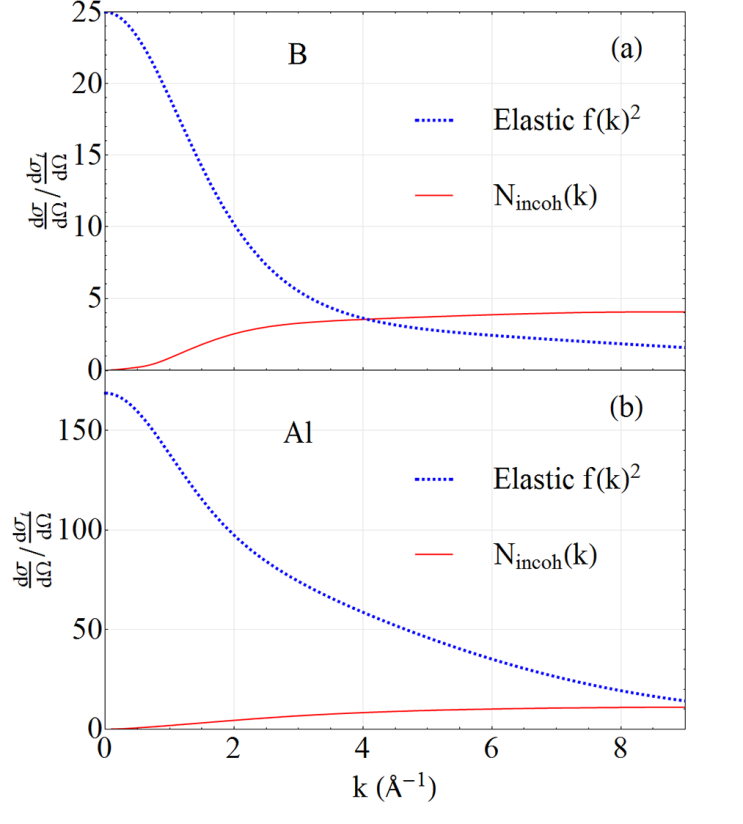
\includegraphics[scale=1.0]{media/image5.png}
\end{figure}

\FloatBarrier

\begin{figure}[h] 
\caption{ Red: experimental thermal
backlighter spectrum from OMEGA
\hyperref[b.-yaakobi-2012-private-communication.]{\textsuperscript{43}}\emph{.}
Blue: a short-pulse Cu \emph{K\textsubscript{α}} backlighter spectrum,
based on scaling of results from a lower energy laser system to a 2.5
kJ, 10 ps laser shot at OMEGA
\hyperref[p.-m.-nilson-2012-private-communication.]{\textsuperscript{44}}\textsuperscript{,}
\hyperref[k.-u.-akli-et-al.-physics-of-plasmas-14-023102-2007.]{\textsuperscript{45}}\hyperref[b.-a.-mattern-g.-t.-seidler-j.-j.-kas-j.-i.-pacold-and-j.-j.-rehr-physical-review-b-85-115135-2012.]{}.}
\label{edimage3}
\centering
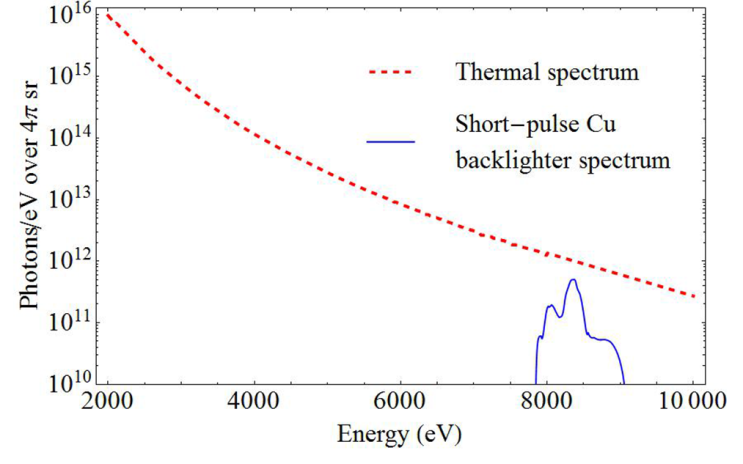
\includegraphics[scale=1.0]{media/image3.png}
\end{figure}

In Fig. \ref{edimage8} we present \(I_{d}\left( E \right)\) defined in section II,
filtered by a 20 µm Be foil (to reject low-energy photons) for liquid
boron acquired on a CCD alongside the equivalent HOPG source spectrum.
The highlighted region of the HOPG source spectrum shows the energy
range covered by a specific configuration: a 12-cm long HOPG crystal at
distance \(F\) = 25 cm from the target, oriented such that the detected
spectrum is centered on the main correlation peak in \(S(k)\). This
crystal size results in a solid angle subtended by the crystal similar
to that in existing high-efficiency HOPG spectrometers
\hyperref[b.-yaakobi-2012-private-communication.]{\textsuperscript{43}}\textsuperscript{,}
\hyperref[a.-pak-g.-gregori-j.-knight-k.-campbell-d.-price-b.-hammel-o.-l.-landen-and-s.-h.-glenzer-review-of-scientific-instruments-75-3747-2004.]{\textsuperscript{61}}.
Figure \ref{edimage9} shows the CCD and HOPG spectra for shock-compressed Al in this
same format. \(S\left( k \right)\) reconstructed for B and Al is
presented in Figs. \ref{edimage10} and 11, respectively. In both these figures the
\(k\)-range probed by the specific spectrometer configuration is
highlighted. All reconstructed \(S\left( k \right)\) curves, including
those without background subtraction, show a well-defined correlation
peak. Note that the uncorrected curves overshoot the experimental
\(S\left( k \right)\) at large \(k\); this is a result of the
monotonically-increasing Compton background (as well as double-counts,
for the CCD). This background decreases relative to the XRD signal for
larger atomic numbers, as seen by comparison of Figs. \ref{edimage10} and 11. The
HOPG source spectrum exhibits excellent statistics (error bars
\textless{} 2 percent) relative to the CCD over the entire plotted
energy range. While deteriorating at high energy, the CCD spectrum also
has good statistics (error bars \textless{} 5 percent) below 4.5 keV.

\begin{figure}[h] 
\caption{ Photon-energy histograms on
CCD and HOPG spectrometers for shock-compressed Al at electron density
\(n_{e}\) = 5.4 × 10\textsuperscript{23} cm\textsuperscript{-3} and
temperature \(T_{e}\) = 10 eV, using Ma \emph{et al.}'s best-fitting
theoretical model to their experimental results for \({f(k)}^{2}\)
\(S(k)\)
\hyperref[t.-ma-et-al.-physical-review-letters-110-065001-2013.]{\textsuperscript{35}},
and assuming \(f(k)\) of ambient Al. The expectation value of photon
counts/pixel on the CCD is \(p\) \emph{=} 0.1. The energy range of a
specific HOPG configuration using a 12-cm long HOPG analyzer is denoted
by the shaded region, the width of which corresponds to the spectrometer
configuration of Fig. 7 (a). The spectrometer's focal length is 25 cm,
and the length of the crystal in the non-energy dispersive orientation
is 12 cm; both spectrometers are positioned at \(2\theta = 135\) deg. A
20-µm thick Be foil is used to reject low-energy photons. Error bars in
the HOPG histogram are smaller than 1\% (not shown).}
\label{edimage9}
\centering
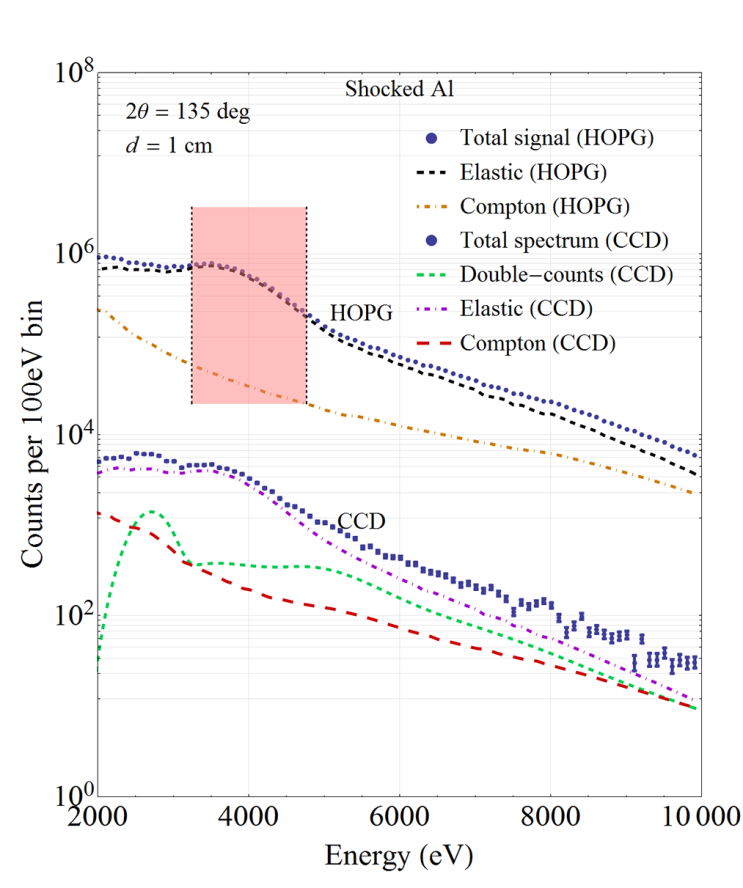
\includegraphics[scale=1.0]{media/image9.png}
\end{figure}

\begin{figure}[h] 
\caption{ Photon-energy histograms for energy-dispersive diffraction
spectra of liquid boron on CCD and HOPG spectrometers. The expectation
value of photon counts/pixel on the CCD is \(p\) \emph{=} 0.1. The
energy range of a specific HOPG configuration using a 12-cm long HOPG
analyzer is denoted by the shaded region, the width of which corresponds
to the spectrometer configuration of Fig. 7 (a). The spectrometer's
focal length is 25 cm, and the length of the crystal in the non-energy
dispersive orientation is 12 cm; both spectrometers are positioned at
\(2\theta = 135\) deg. A 20-µm thick Be foil is used to reject
low-energy photons. Error bars in the HOPG histogram are smaller than
the size of the symbols.}
\label{edimage8}
\centering
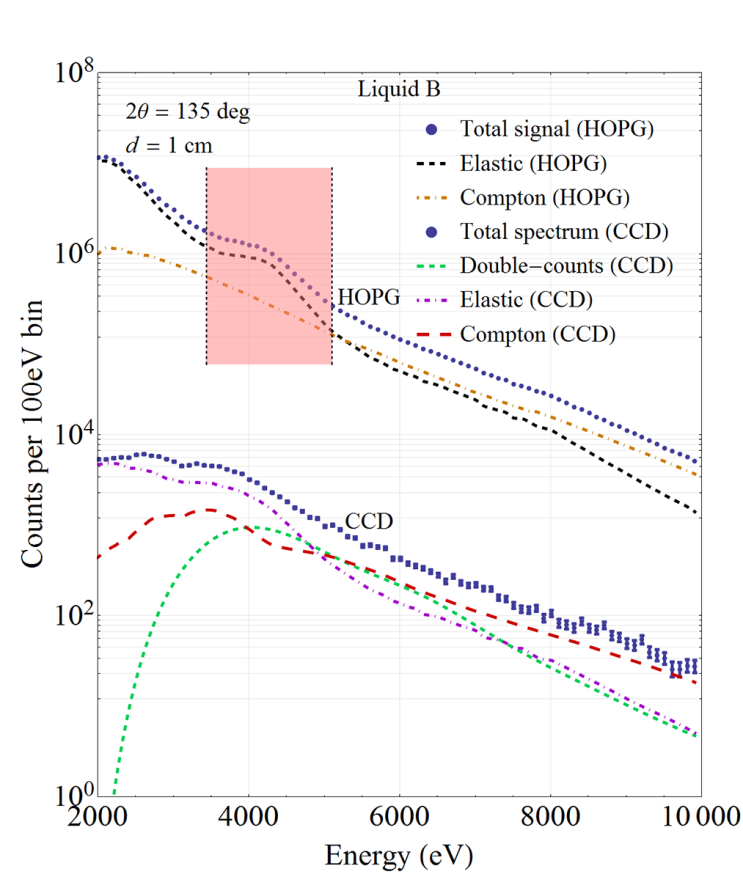
\includegraphics[scale=1.0]{media/image8.png}
\end{figure}

The relative merits of the two detectors are dictated by particular
features of the ED-XRD configuration and the spectrum probed. Despite
the substantially better energy resolution of an HOPG spectrometer
compared to a Fano-noise limited CCD, energy resolution is a poor
criterion for comparison: at 135 degrees scattering angle, the
\(k\)-width of features in \(S(k)\) corresponds to a width in energy
greater than 500 eV, substantially larger than the resolution of both
the CCD and the HOPG spectrometer. Instead, the leading limitation on
data quality is shot noise at high \(k\) due to the sharp decay of the
source spectrum intensity with increasing energy.

The latter limitation is severe only for the CCD, (1) because of vastly
lower overall counts and especially (2) because the intense low-energy
portion of the incident spectrum is `echoed' as double-counts at higher
energy. In simulated CCD spectra the double-count contribution to the
detected spectrum outweighed the single-count contribution above 5 keV.
This double-count noise cannot be reduced by varying \(p\): in the
single photon-hit regime, the number of double-hits on single pixels
scales as \(p^{2}\); the associated Poisson noise scales as \(p\).
Single photon counts also scale as \(p\); as a result, above 5 keV
varying \(p\) has little effect on the signal-to-noise (\emph{i.e.}
single-to-double-count) ratio. It is instead highly preferable to carry
out an ED-XRD experiment in near-backscatter geometry, such that the
range of \(k\) in which \(S(k)\) has structure is probed by a
lower-energy region of the backlighter spectrum. In fact, the only means
of significantly improving data quality on a single hit CCD are (1)
using a detector with more pixels to improve statistics, and (2) moving
the detector closer to backscatter.

The two spectrometer types offer a variety of configurations adapted to
experimental situations in which different \(k\)-ranges need to be
probed. If the goal is to locate the main correlation peak in
\(S(k)\)\emph{,} a single-HOPG crystal spectrometer is a viable option
(illustrated, as mentioned above, in Figs. \ref{edimage10} and \ref{edimage11}). On the other
hand, if the scientific goal requires a significantly wider \(k\)-range,
then a CCD detector in single photon counting mode, multiple HOPG
analyzer crystals, or both are necessary. Despite the CCD's relatively
poor signal to noise ratio, there is substantial motivation for
performing ED-XRD using both spectrometer types if the full \(k\) range
is desired. In such a dual configuration the CCD would provide low-noise
data up to approximately 4.5 keV with one or more HOPG spectrometers
covering the remainder of the energy spectrum, corresponding to a
reduced range of \(\theta_{B}\) from 21 to 49 degrees, for which a
modest number of analyzer crystals would be required.


\begin{figure} 
\caption{ \(S(k)\) for liquid boron
reconstructed from simulated energy-dispersive spectra of Fig. 8 for (a)
an HOPG spectrometer and (b) a CCD, with and without subtraction of
Compton background and photon double-counts. Data bin size is 100 eV.
The shaded \(k\)-range in the HOPG spectrum corresponds to the
spectrometer configuration described in the text, and is centered about
the main correlation peak in \(S(k)\).}
\label{edimage10}
\centering
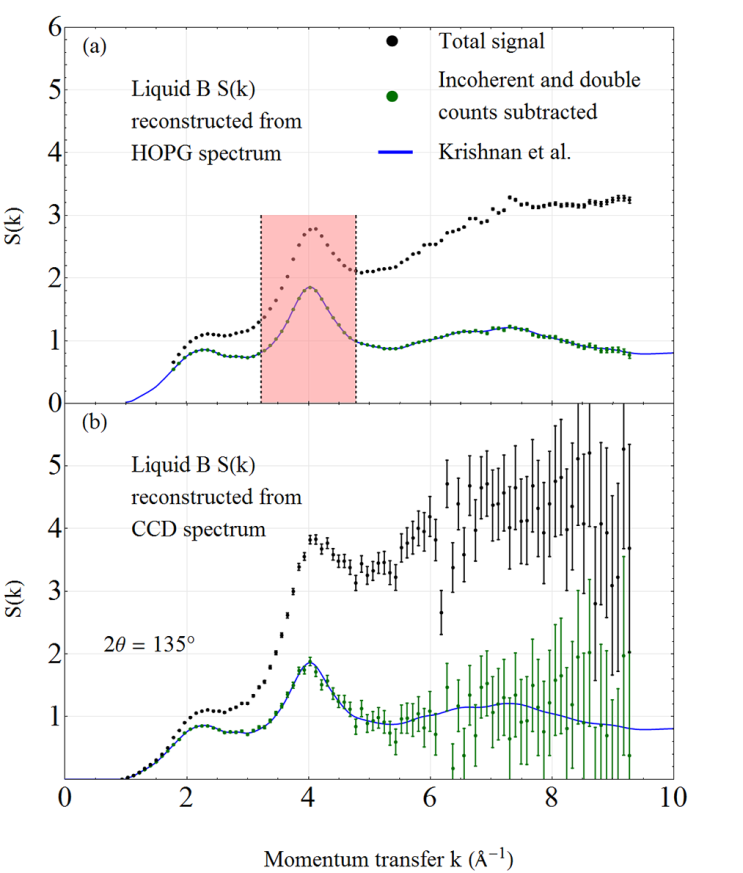
\includegraphics[scale=1.0]{media/image10.png}
\end{figure}

\begin{figure}[h] 
\hyperdef{}{ux5fRef350528323}{}{}
\caption{ In blue: X-ray structure factor \(S(k)\) for shock-compressed
Al computed from Ma, \emph{et al.}
\hyperref[t.-ma-et-al.-physical-review-letters-110-065001-2013.]{\textsuperscript{35}}.
Overlaid with \(S(k)\) reconstructed from the spectra of Fig. 9 for (a)
an HOPG spectrometer and (b) a CCD. The data bin size is 100 eV. The
shaded \(k\)-range in the HOPG spectrum corresponds to the spectrometer
configuration described in the text and is centered about the main
correlation peak in \(S(k)\).}
\label{edimage11}
\centering
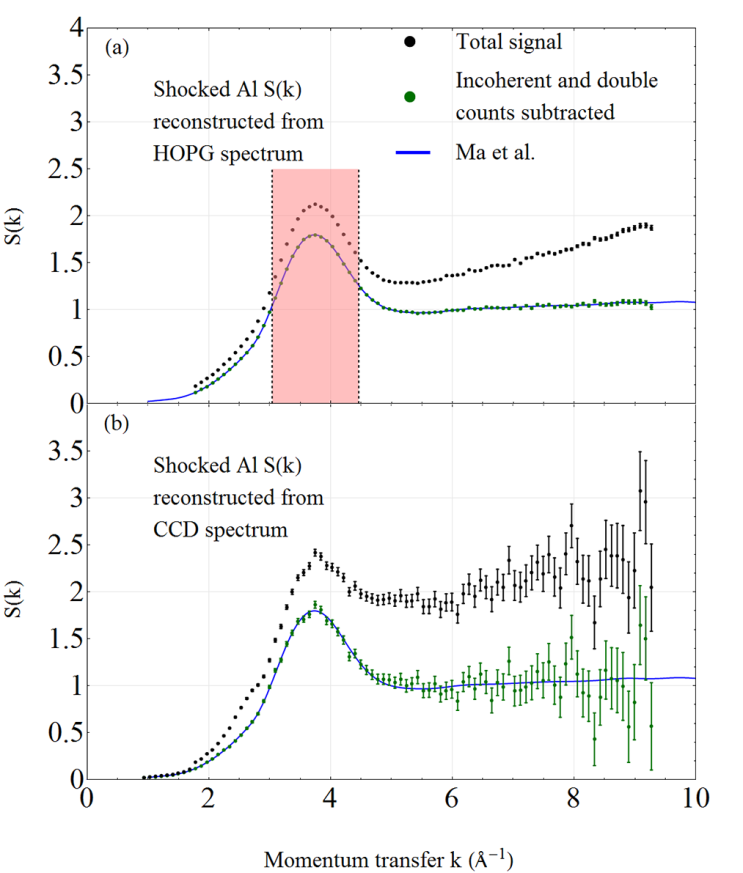
\includegraphics[scale=1.0]{media/image11.png}
\end{figure}



The above results establish single-shot ED-XRD as a viable method for
use at OMEGA, even for systems with only liquid-like, isotropic
short-range order; this observation clearly extends to fine, isotropic
polycrystalline systems where the structure in \(S(k)\) can only be
sharper. We note that pump laser energy is 30 times larger at NIF than
at OMEGA and that the ratio of backlighter fluences exceeds that factor
due to the higher backlighter electron temperature at NIF
\hyperref[b.-r.-maddox-et-al.-physics-of-plasmas-18-056709-2011.]{\textsuperscript{41}}.
Consequently, ED-XRD is also viable at NIF where the higher backlighter
fluence may allow a substantial reduction in solid angle subtended by an
HOPG spectrometer, compared to present calculations. This would in turn
allow incorporating a larger number of spectrometers in a single
diagnostic module. CCD-based studies at NIF are also, in principle,
viable but may run into technical difficulties related to neutron
backgrounds or difficulty in shielding from electromagnetic pulses.

\FloatBarrier

\section{IV. Conclusions}

We report a photometric study of the viability of single-shot
investigation of the isotropic static structure factor \(S(k)\) in
experiments using a broadband x-ray backlighter as the source for
energy-dispersive x-ray diffraction (ED-XRD). The results are extremely
favorable, and indicate that single-shot ED-XRD can be used at OMEGA or
NIF. A standard scientific-grade x-ray CCD camera operating in
single-photon counting mode suffices for many studies, but exhibits
degraded performance at high momentum transfers due to the rapid
decrease of incident flux at higher photon energy. On the other hand, a
typical HOPG-based wavelength dispersive spectrometer has exceptional
count rates in any selected \(k\) range, but its limited energy range
may require either the use of multiple spectrometers or of a single
compound spectrometer having multiple analyzer crystals.


\section{Acknowledgements} We thank Brian Mattern, Tilo Doeppner, Philip Nilson, Barukh Yaakobi,
Christian Stoeckl, Yuan Ping, Justin Wark, and Andrew Higginbotham for
helpful discussions. This work was supported by the US Department of
Energy, Office of Science, Fusion Energy Sciences and the National
Nuclear Security Administration, through grant DE-SC0008580.

% TODO fix references
\section{References}\label{references}
\hyperdef{}{j.-d.-lindl-p.-amendt-r.-l.-berger-s.-g.-glendinning-s.-h.-glenzer-s.-w.-haan-r.-l.-kauffman-o.-l.-landen-and-l.-j.-suter-physics-of-plasmas-11-339-2004.}{\subsection{\texorpdfstring{\textsuperscript{1}
J. D. Lindl, P. Amendt, R. L. Berger, S. G. Glendinning, S. H. Glenzer,
S. W. Haan, R. L. Kauffman, O. L. Landen, and L. J. Suter, Physics of
Plasmas 11, 339
(2004).}{1 J. D. Lindl, P. Amendt, R. L. Berger, S. G. Glendinning, S. H. Glenzer, S. W. Haan, R. L. Kauffman, O. L. Landen, and L. J. Suter, Physics of Plasmas 11, 339 (2004).}}\label{j.-d.-lindl-p.-amendt-r.-l.-berger-s.-g.-glendinning-s.-h.-glenzer-s.-w.-haan-r.-l.-kauffman-o.-l.-landen-and-l.-j.-suter-physics-of-plasmas-11-339-2004.}}

\hyperdef{}{e.-i.-moses-nuclear-fusion-49-104022-2009.}{\subsection{\texorpdfstring{\textsuperscript{2}
E. I. Moses, Nuclear Fusion 49, 104022
(2009).}{2 E. I. Moses, Nuclear Fusion 49, 104022 (2009).}}\label{e.-i.-moses-nuclear-fusion-49-104022-2009.}}

\hyperdef{}{f.-langenhorst-m.-boustie-a.-migault-and-j.-p.-romain-earth-and-planetary-science-letters-173-333-1999.}{\subsection{\texorpdfstring{\textsuperscript{3}
F. Langenhorst, M. Boustie, A. Migault, and J. P. Romain, Earth and
Planetary Science Letters 173, 333
(1999).}{3 F. Langenhorst, M. Boustie, A. Migault, and J. P. Romain, Earth and Planetary Science Letters 173, 333 (1999).}}\label{f.-langenhorst-m.-boustie-a.-migault-and-j.-p.-romain-earth-and-planetary-science-letters-173-333-1999.}}

\subsection{\texorpdfstring{\textsuperscript{4} J. Gattacceca, M.
Boustie, E. Lima, B. P. Weiss, T. de Resseguier, and J. P.
Cuq-Lelandais, Physics of the Earth and Planetary Interiors 182, 42
(2010).}{4 J. Gattacceca, M. Boustie, E. Lima, B. P. Weiss, T. de Resseguier, and J. P. Cuq-Lelandais, Physics of the Earth and Planetary Interiors 182, 42 (2010).}}\label{j.-gattacceca-m.-boustie-e.-lima-b.-p.-weiss-t.-de-resseguier-and-j.-p.-cuq-lelandais-physics-of-the-earth-and-planetary-interiors-182-42-2010.}

\subsection{\texorpdfstring{\textsuperscript{5} H. Takabe, et al.,
Plasma Physics and Controlled Fusion 50, 124057
(2008).}{5 H. Takabe, et al., Plasma Physics and Controlled Fusion 50, 124057 (2008).}}\label{h.-takabe-et-al.-plasma-physics-and-controlled-fusion-50-124057-2008.}

\subsection{\texorpdfstring{\textsuperscript{6} L. O. Silva, M. Marti,
J. R. Davies, R. A. Fonseca, C. Ren, F. S. Tsung, and W. B. Mori,
Physical Review Letters 92, 015002
(2004).}{6 L. O. Silva, M. Marti, J. R. Davies, R. A. Fonseca, C. Ren, F. S. Tsung, and W. B. Mori, Physical Review Letters 92, 015002 (2004).}}\label{l.-o.-silva-m.-marti-j.-r.-davies-r.-a.-fonseca-c.-ren-f.-s.-tsung-and-w.-b.-mori-physical-review-letters-92-015002-2004.}

\subsection{\texorpdfstring{\textsuperscript{7} B. A. Remington, R. P.
Drake, H. Takabe, and D. Arnett, Physics of Plasmas 7, 1641
(2000).}{7 B. A. Remington, R. P. Drake, H. Takabe, and D. Arnett, Physics of Plasmas 7, 1641 (2000).}}\label{b.-a.-remington-r.-p.-drake-h.-takabe-and-d.-arnett-physics-of-plasmas-7-1641-2000.}

\subsection{\texorpdfstring{\textsuperscript{8} H.-S. Park, et al., High
Energy Density Physics 8, 38
(2012).}{8 H.-S. Park, et al., High Energy Density Physics 8, 38 (2012).}}\label{h.-s.-park-et-al.-high-energy-density-physics-8-38-2012.}

\subsection{\texorpdfstring{\textsuperscript{9} M. Koenig, et al.,
Physics of Plasmas 13, 056504
(2006).}{9 M. Koenig, et al., Physics of Plasmas 13, 056504 (2006).}}\label{m.-koenig-et-al.-physics-of-plasmas-13-056504-2006.}

\subsection{\texorpdfstring{\textsuperscript{10} A. Macchi, M. Borghesi,
and M. Passoni, Reviews of Modern Physics 85, 751
(2013).}{10 A. Macchi, M. Borghesi, and M. Passoni, Reviews of Modern Physics 85, 751 (2013).}}\label{a.-macchi-m.-borghesi-and-m.-passoni-reviews-of-modern-physics-85-751-2013.}

\subsection{\texorpdfstring{\textsuperscript{11} G. Gregori, et al.,
Nature 481, 480
(2012).}{11 G. Gregori, et al., Nature 481, 480 (2012).}}\label{g.-gregori-et-al.-nature-481-480-2012.}

\subsection{\texorpdfstring{\textsuperscript{12} F. Fiuza, R. A.
Fonseca, J. Tonge, W. B. Mori, and L. O. Silva, Physical Review Letters
108, 235004
(2012).}{12 F. Fiuza, R. A. Fonseca, J. Tonge, W. B. Mori, and L. O. Silva, Physical Review Letters 108, 235004 (2012).}}\label{f.-fiuza-r.-a.-fonseca-j.-tonge-w.-b.-mori-and-l.-o.-silva-physical-review-letters-108-235004-2012.}

\subsection{\texorpdfstring{\textsuperscript{13} F. Dollar, et al.,
Physical Review Letters 110, 175002
(2013).}{13 F. Dollar, et al., Physical Review Letters 110, 175002 (2013).}}\label{f.-dollar-et-al.-physical-review-letters-110-175002-2013.}

\subsection{\texorpdfstring{\textsuperscript{14} K. U. Akli, et al.,
Physical Review Letters 100, 165002
(2008).}{14 K. U. Akli, et al., Physical Review Letters 100, 165002 (2008).}}\label{k.-u.-akli-et-al.-physical-review-letters-100-165002-2008.}

\hyperdef{}{b.-k.-f.-young-et-al.-review-of-scientific-instruments-69-4049-1998.}{\subsection{\texorpdfstring{\textsuperscript{15}
B. K. F. Young, et al., Review of Scientific Instruments 69, 4049
(1998).}{15 B. K. F. Young, et al., Review of Scientific Instruments 69, 4049 (1998).}}\label{b.-k.-f.-young-et-al.-review-of-scientific-instruments-69-4049-1998.}}

\subsection{\texorpdfstring{\textsuperscript{16} K. Oades, A. Evans, G.
Slark, J. Foster, R. Eagleton, and E. Clark, Review of Scientific
Instruments 75, 4222
(2004).}{16 K. Oades, A. Evans, G. Slark, J. Foster, R. Eagleton, and E. Clark, Review of Scientific Instruments 75, 4222 (2004).}}\label{k.-oades-a.-evans-g.-slark-j.-foster-r.-eagleton-and-e.-clark-review-of-scientific-instruments-75-4222-2004.}

\subsection{\texorpdfstring{\textsuperscript{17} J. Workman and G. A.
Kyrala, Review of Scientific Instruments 72, 678
(2001).}{17 J. Workman and G. A. Kyrala, Review of Scientific Instruments 72, 678 (2001).}}\label{j.-workman-and-g.-a.-kyrala-review-of-scientific-instruments-72-678-2001.}

\subsection{\texorpdfstring{\textsuperscript{18} C. Stoeckl, V. Y.
Glebov, D. D. Meyerhofer, W. Seka, B. Yaakobi, R. P. J. Town, and J. D.
Zuegel, Review of Scientific Instruments 72, 1197
(2001).}{18 C. Stoeckl, V. Y. Glebov, D. D. Meyerhofer, W. Seka, B. Yaakobi, R. P. J. Town, and J. D. Zuegel, Review of Scientific Instruments 72, 1197 (2001).}}\label{c.-stoeckl-v.-y.-glebov-d.-d.-meyerhofer-w.-seka-b.-yaakobi-r.-p.-j.-town-and-j.-d.-zuegel-review-of-scientific-instruments-72-1197-2001.}

\subsection{\texorpdfstring{\textsuperscript{19} C. Sorce, et al.,
Review of Scientific Instruments 77, 10E518
(2006).}{19 C. Sorce, et al., Review of Scientific Instruments 77, 10E518 (2006).}}\label{c.-sorce-et-al.-review-of-scientific-instruments-77-10e518-2006.}

\subsection{\texorpdfstring{\textsuperscript{20} J. A. Oertel, et al.,
Review of Scientific Instruments 77, 10E308
(2006).}{20 J. A. Oertel, et al., Review of Scientific Instruments 77, 10E308 (2006).}}\label{j.-a.-oertel-et-al.-review-of-scientific-instruments-77-10e308-2006.}

\subsection{\texorpdfstring{\textsuperscript{21} O. L. Landen, et al.,
Review of Scientific Instruments 72, 627
(2001).}{21 O. L. Landen, et al., Review of Scientific Instruments 72, 627 (2001).}}\label{o.-l.-landen-et-al.-review-of-scientific-instruments-72-627-2001.}

\subsection{\texorpdfstring{\textsuperscript{22} L. T. Hudson, A.
Henins, R. D. Deslattes, J. F. Seely, G. E. Holland, R. Atkin, L.
Marlin, D. D. Meyerhofer, and C. Stoeckl, Review of Scientific
Instruments 73, 2270
(2002).}{22 L. T. Hudson, A. Henins, R. D. Deslattes, J. F. Seely, G. E. Holland, R. Atkin, L. Marlin, D. D. Meyerhofer, and C. Stoeckl, Review of Scientific Instruments 73, 2270 (2002).}}\label{l.-t.-hudson-a.-henins-r.-d.-deslattes-j.-f.-seely-g.-e.-holland-r.-atkin-l.-marlin-d.-d.-meyerhofer-and-c.-stoeckl-review-of-scientific-instruments-73-2270-2002.}

\subsection{\texorpdfstring{\textsuperscript{23} E. L. Dewald, et al.,
Review of Scientific Instruments 75, 3759
(2004).}{23 E. L. Dewald, et al., Review of Scientific Instruments 75, 3759 (2004).}}\label{e.-l.-dewald-et-al.-review-of-scientific-instruments-75-3759-2004.}

\subsection{\texorpdfstring{\textsuperscript{24} T. Doeppner, P.
Neumayer, F. Girard, N. L. Kugland, O. L. Landen, C. Niemann, and S. H.
Glenzer, Review of Scientific Instruments 79, 10E311
(2008).}{24 T. Doeppner, P. Neumayer, F. Girard, N. L. Kugland, O. L. Landen, C. Niemann, and S. H. Glenzer, Review of Scientific Instruments 79, 10E311 (2008).}}\label{t.-doeppner-p.-neumayer-f.-girard-n.-l.-kugland-o.-l.-landen-c.-niemann-and-s.-h.-glenzer-review-of-scientific-instruments-79-10e311-2008.}

\hyperdef{}{s.-h.-glenzer-and-r.-redmer-reviews-of-modern-physics-81-1625-2009.}{\subsection{\texorpdfstring{\textsuperscript{25}
S. H. Glenzer and R. Redmer, Reviews of Modern Physics 81, 1625
(2009).}{25 S. H. Glenzer and R. Redmer, Reviews of Modern Physics 81, 1625 (2009).}}\label{s.-h.-glenzer-and-r.-redmer-reviews-of-modern-physics-81-1625-2009.}}

\hyperdef{}{g.-gregori-et-al.-physics-of-plasmas-11-2754-2004.}{\subsection{\texorpdfstring{\textsuperscript{26}
G. Gregori, et al., Physics of Plasmas 11, 2754
(2004).}{26 G. Gregori, et al., Physics of Plasmas 11, 2754 (2004).}}\label{g.-gregori-et-al.-physics-of-plasmas-11-2754-2004.}}

\hyperdef{}{h.-j.-lee-et-al.-physical-review-letters-102-115001-2009.}{\subsection{\texorpdfstring{\textsuperscript{27}
H. J. Lee, et al., Physical Review Letters 102, 115001
(2009).}{27 H. J. Lee, et al., Physical Review Letters 102, 115001 (2009).}}\label{h.-j.-lee-et-al.-physical-review-letters-102-115001-2009.}}

\hyperdef{}{c.-fortmann-h.-j.-lee-t.-doeppner-r.-w.-falcone-a.-l.-kritcher-o.-l.-landen-and-s.-h.-glenzer-physical-review-letters-108-175006-2012.}{\subsection{\texorpdfstring{\textsuperscript{28}
C. Fortmann, H. J. Lee, T. Doeppner, R. W. Falcone, A. L. Kritcher, O.
L. Landen, and S. H. Glenzer, Physical Review Letters 108, 175006
(2012).}{28 C. Fortmann, H. J. Lee, T. Doeppner, R. W. Falcone, A. L. Kritcher, O. L. Landen, and S. H. Glenzer, Physical Review Letters 108, 175006 (2012).}}\label{c.-fortmann-h.-j.-lee-t.-doeppner-r.-w.-falcone-a.-l.-kritcher-o.-l.-landen-and-s.-h.-glenzer-physical-review-letters-108-175006-2012.}}

\subsection{\texorpdfstring{\textsuperscript{29} B. A. Mattern, G. T.
Seidler, and J. J. Kas, arXiv:1308.2990
(2013).}{29 B. A. Mattern, G. T. Seidler, and J. J. Kas, arXiv:1308.2990 (2013).}}\label{b.-a.-mattern-g.-t.-seidler-and-j.-j.-kas-arxiv1308.2990-2013.}

\hyperdef{}{v.-lider-crystallography-reports-56-169-2011.}{\subsection{\texorpdfstring{\textsuperscript{30}
V. Lider, Crystallography Reports 56, 169
(2011).}{30 V. Lider, Crystallography Reports 56, 169 (2011).}}\label{v.-lider-crystallography-reports-56-169-2011.}}

\hyperdef{}{m.-suggit-g.-kimminau-j.-hawreliak-b.-remington-n.-park-and-j.-wark-review-of-scientific-instruments-81-083902-2010.}{\subsection{\texorpdfstring{\textsuperscript{31}
M. Suggit, G. Kimminau, J. Hawreliak, B. Remington, N. Park, and J.
Wark, Review of Scientific Instruments 81, 083902
(2010).}{31 M. Suggit, G. Kimminau, J. Hawreliak, B. Remington, N. Park, and J. Wark, Review of Scientific Instruments 81, 083902 (2010).}}\label{m.-suggit-g.-kimminau-j.-hawreliak-b.-remington-n.-park-and-j.-wark-review-of-scientific-instruments-81-083902-2010.}}

\hyperdef{}{m.-j.-suggit-et-al.-nature-communications-3-1224-2012.}{\subsection{\texorpdfstring{\textsuperscript{32}
M. J. Suggit, et al., Nature Communications 3, 1224
(2012).}{32 M. J. Suggit, et al., Nature Communications 3, 1224 (2012).}}\label{m.-j.-suggit-et-al.-nature-communications-3-1224-2012.}}

\hyperdef{}{b.-yaakobi-t.-r.-boehly-d.-d.-meyerhofer-t.-j.-b.-collins-b.-a.-remington-p.-g.-allen-s.-m.-pollaine-h.-e.-lorenzana-and-j.-h.-eggert-physical-review-letters-95-075501-2005.}{\subsection{\texorpdfstring{\textsuperscript{33}
B. Yaakobi, T. R. Boehly, D. D. Meyerhofer, T. J. B. Collins, B. A.
Remington, P. G. Allen, S. M. Pollaine, H. E. Lorenzana, and J. H.
Eggert, Physical Review Letters 95, 075501
(2005).}{33 B. Yaakobi, T. R. Boehly, D. D. Meyerhofer, T. J. B. Collins, B. A. Remington, P. G. Allen, S. M. Pollaine, H. E. Lorenzana, and J. H. Eggert, Physical Review Letters 95, 075501 (2005).}}\label{b.-yaakobi-t.-r.-boehly-d.-d.-meyerhofer-t.-j.-b.-collins-b.-a.-remington-p.-g.-allen-s.-m.-pollaine-h.-e.-lorenzana-and-j.-h.-eggert-physical-review-letters-95-075501-2005.}}

\hyperdef{}{j.-l.-bourgade-et-al.-review-of-scientific-instruments-75-4204-2004.}{\subsection{\texorpdfstring{\textsuperscript{34}
J. L. Bourgade, et al., Review of Scientific Instruments 75, 4204
(2004).}{34 J. L. Bourgade, et al., Review of Scientific Instruments 75, 4204 (2004).}}\label{j.-l.-bourgade-et-al.-review-of-scientific-instruments-75-4204-2004.}}

\hyperdef{}{t.-ma-et-al.-physical-review-letters-110-065001-2013.}{\subsection{\texorpdfstring{\textsuperscript{35}
T. Ma, et al., Physical Review Letters 110, 065001
(2013).}{35 T. Ma, et al., Physical Review Letters 110, 065001 (2013).}}\label{t.-ma-et-al.-physical-review-letters-110-065001-2013.}}

\hyperdef{}{y.-feng-m.-somayazulu-r.-jaramillo-t.-rosenbaum-e.-isaacs-j.-hu-and-h.-k.-mao-review-of-scientific-instruments-76-063913-2005.}{\subsection{\texorpdfstring{\textsuperscript{36}
Y. Feng, M. Somayazulu, R. Jaramillo, T. Rosenbaum, E. Isaacs, J. Hu,
and H.-k. Mao, Review of Scientific Instruments 76, 063913
(2005).}{36 Y. Feng, M. Somayazulu, R. Jaramillo, T. Rosenbaum, E. Isaacs, J. Hu, and H.-k. Mao, Review of Scientific Instruments 76, 063913 (2005).}}\label{y.-feng-m.-somayazulu-r.-jaramillo-t.-rosenbaum-e.-isaacs-j.-hu-and-h.-k.-mao-review-of-scientific-instruments-76-063913-2005.}}

\subsection{\texorpdfstring{\textsuperscript{37} E. J. Mittemeijer and
U. Welzel, \emph{Modern Diffraction Methods} (Wiley-VCH,
2012).}{37 E. J. Mittemeijer and U. Welzel, Modern Diffraction Methods (Wiley-VCH, 2012).}}\label{e.-j.-mittemeijer-and-u.-welzel-modern-diffraction-methods-wiley-vch-2012.}

\subsection{\texorpdfstring{\textsuperscript{38} Y. Feng, et al.,
Physical Review Letters 99, 137201
(2007).}{38 Y. Feng, et al., Physical Review Letters 99, 137201 (2007).}}\label{y.-feng-et-al.-physical-review-letters-99-137201-2007.}

\subsection{\texorpdfstring{\textsuperscript{39} S. Desgreniers, Y. K.
Vohra, and A. L. Ruoff, Physical Review B 39, 10359
(1989).}{39 S. Desgreniers, Y. K. Vohra, and A. L. Ruoff, Physical Review B 39, 10359 (1989).}}\label{s.-desgreniers-y.-k.-vohra-and-a.-l.-ruoff-physical-review-b-39-10359-1989.}

\subsection{\texorpdfstring{\textsuperscript{40} M. A. Baublitz, V.
Arnold, and A. L. Ruoff, Review of Scientific Instruments 52, 1616
(1981).}{40 M. A. Baublitz, V. Arnold, and A. L. Ruoff, Review of Scientific Instruments 52, 1616 (1981).}}\label{m.-a.-baublitz-v.-arnold-and-a.-l.-ruoff-review-of-scientific-instruments-52-1616-1981.}

\hyperdef{}{b.-r.-maddox-et-al.-physics-of-plasmas-18-056709-2011.}{\subsection{\texorpdfstring{\textsuperscript{41}
B. R. Maddox, et al., Physics of Plasmas 18, 056709
(2011).}{41 B. R. Maddox, et al., Physics of Plasmas 18, 056709 (2011).}}\label{b.-r.-maddox-et-al.-physics-of-plasmas-18-056709-2011.}}

\hyperdef{}{b.-yaakobi-f.-j.-marshall-t.-r.-boehly-r.-p.-j.-town-and-d.-d.-meyerhofer-journal-of-the-optical-society-of-america-b-optical-physics-20-238-2003.}{\subsection{\texorpdfstring{\textsuperscript{42}
B. Yaakobi, F. J. Marshall, T. R. Boehly, R. P. J. Town, and D. D.
Meyerhofer, Journal of the Optical Society of America B-Optical Physics
20, 238
(2003).}{42 B. Yaakobi, F. J. Marshall, T. R. Boehly, R. P. J. Town, and D. D. Meyerhofer, Journal of the Optical Society of America B-Optical Physics 20, 238 (2003).}}\label{b.-yaakobi-f.-j.-marshall-t.-r.-boehly-r.-p.-j.-town-and-d.-d.-meyerhofer-journal-of-the-optical-society-of-america-b-optical-physics-20-238-2003.}}

\hyperdef{}{b.-yaakobi-2012-private-communication.}{\subsection{\texorpdfstring{\textsuperscript{43}
B. Yaakobi, 2012 (private
communication).}{43 B. Yaakobi, 2012 (private communication).}}\label{b.-yaakobi-2012-private-communication.}}

\hyperdef{}{p.-m.-nilson-2012-private-communication.}{\subsection{\texorpdfstring{\textsuperscript{44}
P. M. Nilson, 2012 (private
communication).}{44 P. M. Nilson, 2012 (private communication).}}\label{p.-m.-nilson-2012-private-communication.}}

\hyperdef{}{k.-u.-akli-et-al.-physics-of-plasmas-14-023102-2007.}{\subsection{\texorpdfstring{\textsuperscript{45}
K. U. Akli, et al., Physics of Plasmas 14, 023102
(2007).}{45 K. U. Akli, et al., Physics of Plasmas 14, 023102 (2007).}}\label{k.-u.-akli-et-al.-physics-of-plasmas-14-023102-2007.}}

\hyperdef{}{s.-krishnan-s.-ansell-j.-j.-felten-k.-j.-volin-and-d.-l.-price-physical-review-letters-81-586-1998.}{\subsection{\texorpdfstring{\textsuperscript{46}
S. Krishnan, S. Ansell, J. J. Felten, K. J. Volin, and D. L. Price,
Physical Review Letters 81, 586
(1998).}{46 S. Krishnan, S. Ansell, J. J. Felten, K. J. Volin, and D. L. Price, Physical Review Letters 81, 586 (1998).}}\label{s.-krishnan-s.-ansell-j.-j.-felten-k.-j.-volin-and-d.-l.-price-physical-review-letters-81-586-1998.}}

\hyperdef{}{s.-krishnan-and-d.-l.-price-journal-of-physics-condensed-matter-12-r145-2000.}{\subsection{\texorpdfstring{\textsuperscript{47}
S. Krishnan and D. L. Price, Journal of Physics-Condensed Matter 12,
R145
(2000).}{47 S. Krishnan and D. L. Price, Journal of Physics-Condensed Matter 12, R145 (2000).}}\label{s.-krishnan-and-d.-l.-price-journal-of-physics-condensed-matter-12-r145-2000.}}

\hyperdef{}{g.-gregori-and-d.-o.-gericke-physics-of-plasmas-16-056306-2009.}{\subsection{\texorpdfstring{\textsuperscript{48}
G. Gregori and D. O. Gericke, Physics of Plasmas 16, 056306
(2009).}{48 G. Gregori and D. O. Gericke, Physics of Plasmas 16, 056306 (2009).}}\label{g.-gregori-and-d.-o.-gericke-physics-of-plasmas-16-056306-2009.}}

\hyperdef{}{j.-chihara-journal-of-physics-condensed-matter-12-231-2000.}{\subsection{\texorpdfstring{\textsuperscript{49}
J. Chihara, Journal of Physics-Condensed Matter 12, 231
(2000).}{49 J. Chihara, Journal of Physics-Condensed Matter 12, 231 (2000).}}\label{j.-chihara-journal-of-physics-condensed-matter-12-231-2000.}}

\hyperdef{}{w.-schuelke-electron-dynamics-by-inelastic-x-ray-scattering-oxford-university-press-new-york-2007.}{\subsection{\texorpdfstring{\textsuperscript{50}
W. Schuelke, \emph{Electron Dynamics by Inelastic X-Ray Scattering}
(Oxford University Press, New York,
2007).}{50 W. Schuelke, Electron Dynamics by Inelastic X-Ray Scattering (Oxford University Press, New York, 2007).}}\label{w.-schuelke-electron-dynamics-by-inelastic-x-ray-scattering-oxford-university-press-new-york-2007.}}

\hyperdef{}{p.-eisenberger-and-p.-m.-platzman-physical-review-a-2-415-1970.}{\subsection{\texorpdfstring{\textsuperscript{51}
P. Eisenberger and P. M. Platzman, Physical Review A 2, 415
(1970).}{51 P. Eisenberger and P. M. Platzman, Physical Review A 2, 415 (1970).}}\label{p.-eisenberger-and-p.-m.-platzman-physical-review-a-2-415-1970.}}

\hyperdef{}{b.-a.-mattern-g.-t.-seidler-j.-j.-kas-j.-i.-pacold-and-j.-j.-rehr-physical-review-b-85-115135-2012.}{\subsection{\texorpdfstring{\textsuperscript{52}
B. A. Mattern, G. T. Seidler, J. J. Kas, J. I. Pacold, and J. J. Rehr,
Physical Review B 85, 115135
(2012).}{52 B. A. Mattern, G. T. Seidler, J. J. Kas, J. I. Pacold, and J. J. Rehr, Physical Review B 85, 115135 (2012).}}\label{b.-a.-mattern-g.-t.-seidler-j.-j.-kas-j.-i.-pacold-and-j.-j.-rehr-physical-review-b-85-115135-2012.}}

\subsection{\texorpdfstring{\textsuperscript{53} Y. Jae-Hyuck, I. Jung
Bin, P. Jong Bok, J. Hojeong, and P. G. Costas, Applied Physics Letters
100, 233124
(2012).}{53 Y. Jae-Hyuck, I. Jung Bin, P. Jong Bok, J. Hojeong, and P. G. Costas, Applied Physics Letters 100, 233124 (2012).}}\label{y.-jae-hyuck-i.-jung-bin-p.-jong-bok-j.-hojeong-and-p.-g.-costas-applied-physics-letters-100-233124-2012.}

\subsection{\texorpdfstring{\textsuperscript{54} A. J. Visco, R. P.
Drake, S. H. Glenzer, T. Doppner, G. Gregori, D. H. Froula, and M. J.
Grosskopf, Physical Review Letters 108, 145001
(2012).}{54 A. J. Visco, R. P. Drake, S. H. Glenzer, T. Doppner, G. Gregori, D. H. Froula, and M. J. Grosskopf, Physical Review Letters 108, 145001 (2012).}}\label{a.-j.-visco-r.-p.-drake-s.-h.-glenzer-t.-doppner-g.-gregori-d.-h.-froula-and-m.-j.-grosskopf-physical-review-letters-108-145001-2012.}

\subsection{\texorpdfstring{\textsuperscript{55} E. J. Gamboa, C. M.
Huntington, M. R. Trantham, P. A. Keiter, R. P. Drake, D. S. Montgomery,
J. F. Benage, and S. A. Letzring, Review of Scientific Instruments 83,
10E108
(2012).}{55 E. J. Gamboa, C. M. Huntington, M. R. Trantham, P. A. Keiter, R. P. Drake, D. S. Montgomery, J. F. Benage, and S. A. Letzring, Review of Scientific Instruments 83, 10E108 (2012).}}\label{e.-j.-gamboa-c.-m.-huntington-m.-r.-trantham-p.-a.-keiter-r.-p.-drake-d.-s.-montgomery-j.-f.-benage-and-s.-a.-letzring-review-of-scientific-instruments-83-10e108-2012.}

\hyperdef{}{a.-k.-freund-a.-munkholm-and-s.-brennan-optics-for-high-brightness-synchrotron-radiation-beamlines-ii-2856-68-1996.}{\subsection{\texorpdfstring{\textsuperscript{56}
A. K. Freund, A. Munkholm, and S. Brennan, Optics for High-Brightness
Synchrotron Radiation Beamlines Ii 2856, 68
(1996).}{56 A. K. Freund, A. Munkholm, and S. Brennan, Optics for High-Brightness Synchrotron Radiation Beamlines Ii 2856, 68 (1996).}}\label{a.-k.-freund-a.-munkholm-and-s.-brennan-optics-for-high-brightness-synchrotron-radiation-beamlines-ii-2856-68-1996.}}

\hyperdef{}{r.-tommasini-et-al.-review-of-scientific-instruments-79-10e901-2008.}{\subsection{\texorpdfstring{\textsuperscript{57}
R. Tommasini, et al., Review of Scientific Instruments 79, 10E901
(2008).}{57 R. Tommasini, et al., Review of Scientific Instruments 79, 10E901 (2008).}}\label{r.-tommasini-et-al.-review-of-scientific-instruments-79-10e901-2008.}}

\subsection{\texorpdfstring{\textsuperscript{58} A. L. Kritcher, et al.,
Science 322, 69
(2008).}{58 A. L. Kritcher, et al., Science 322, 69 (2008).}}\label{a.-l.-kritcher-et-al.-science-322-69-2008.}

\subsection{\texorpdfstring{\textsuperscript{59} S. H. Glenzer, G.
Gregori, R. W. Lee, F. J. Rogers, S. W. Pollaine, and O. L. Landen,
Physical Review Letters 90, 175002
(2003).}{59 S. H. Glenzer, G. Gregori, R. W. Lee, F. J. Rogers, S. W. Pollaine, and O. L. Landen, Physical Review Letters 90, 175002 (2003).}}\label{s.-h.-glenzer-g.-gregori-r.-w.-lee-f.-j.-rogers-s.-w.-pollaine-and-o.-l.-landen-physical-review-letters-90-175002-2003.}

\subsection{\texorpdfstring{\textsuperscript{60} G. Gregori, et al.,
Journal of Quantitative Spectroscopy \& Radiative Transfer 99, 225
(2006).}{60 G. Gregori, et al., Journal of Quantitative Spectroscopy \& Radiative Transfer 99, 225 (2006).}}\label{g.-gregori-et-al.-journal-of-quantitative-spectroscopy-radiative-transfer-99-225-2006.}

\hyperdef{}{a.-pak-g.-gregori-j.-knight-k.-campbell-d.-price-b.-hammel-o.-l.-landen-and-s.-h.-glenzer-review-of-scientific-instruments-75-3747-2004.}{\subsection{\texorpdfstring{\textsuperscript{61}
A. Pak, G. Gregori, J. Knight, K. Campbell, D. Price, B. Hammel, O. L.
Landen, and S. H. Glenzer, Review of Scientific Instruments 75, 3747
(2004).}{61 A. Pak, G. Gregori, J. Knight, K. Campbell, D. Price, B. Hammel, O. L. Landen, and S. H. Glenzer, Review of Scientific Instruments 75, 3747 (2004).}}\label{a.-pak-g.-gregori-j.-knight-k.-campbell-d.-price-b.-hammel-o.-l.-landen-and-s.-h.-glenzer-review-of-scientific-instruments-75-3747-2004.}}

\subsection{}\label{section}


















\chapter{X-ray Free Electron Laser-Based Studies of WDM}
\section{X-ray Free Electron Lasers}
XFELs produce radiation of unprecedented brilliance (10 orders of magnitude higher than undulator radiation from third-generation synchrotron sources), full transverse coherence, pulse durations as short as 10 fs. This combination of capability far exceeds that possible with third-generation light sources and opens new frontiers in imaging and the interrogation of ultrafast processes in materials science and biology (cites). In this section we give an overview of the technology and its range of applications in the study of HED states of matter.

\subsection{Physics of XFELs}
To describe the FEL interaction, we first consider the generic case of radiation emission from undulators, the type of insertion device used in both XFELs and the highest-brilliance beamlines at third-generation synchrotron light sources.

A simple time-of-flight argument may be used to obtain an intuitive understanding of radiation by a single electron in an undulator. A radiation wavefront co-propagating with an electron undergoing forced transverse undulation with a (longitudinal) period $\lambda_u$ will move ahead of the electron. Constructive interference of the radiation field produced by successive undulations of the electron will occur at discrete values of the electromagnetic wavelength, $\lambda_n$, satisfying $\lambda_n = \lambda_1 / n$, where $\lambda_1$ is defined as the fundamental resonant wavelength. The time $t$ taken for an electron to propagate one undulator period $\lambda_u$ at speed $v_z$ ($t = \lambda_u/v_z$) is equal to that needed for a resonant wavefront travel the distance $\lambda_u + n \lambda_n$. Equating the propagation times for the wavefront and electron yields the relation (cite McNeil et al.)

\begin{equation}
\lambda_n = \frac{\lambda_u}{n}(\frac{1 - v_z/c}{v_z/c}).
\end{equation}

More detailed treatment shows that, in the case of a helical undulator, only the fundamental mode has strong on-axis emission. (cites)

This describes the narrow spectral width of undulator radiation and the coherent addition of radiated wave amplitudes by a single electron over the length of an undulator. This constructive interference accounts for the much higher brilliance of radiation produced by an undulator, compared to a wiggler or bending magnet. 

At a synchrotron light source electrons in a bunch have uncorrelated positions, and the undulator spectrum is therefore a simple incoherent sum of the emission of all individual electrons passing through it. An XFEL improves on this by creating a positional ordering electrons into `micro-bunches' separated from one another by the radiation field wavelength. The coherent emission from multiple micro-bunches with $N_b$ electrons each would be equivalent, in an idealized case where the micro-bunch dimension were much smaller than the x-ray wavelength, to that from point-like charges of magnitude $e N_b$, with a resulting factor of $N_b^2$ enhancement in brilliance relative to that from an incoherently-emitting electron bunch. (cite)


\begin{figure}[h] 
\caption{Operation of an x-ray free electron laser (cite McNeil). Electrons enter the undulator with random phases and originally emit incoherent radiation at the undulator's resonant wavelength. As the electrons propagates, random fluctuations in the radiation field causes them to bunch at the resonant wavelength and emit coherently.}
\label{fig:xfel}
\centering
\includegraphics[scale=0.5]{../Figures/XFEL.png}
\end{figure}

Electrons in an undulator experience a longitudinal force from the radiation field that is modulated by its period. The consequent bunching of electrons with a period equal to the X-ray wavelength is a self-reinforcing process referred to as self amplified stimulated emission (SASE) (cites). Crucially, the occurrence of SASE requires a sufficiently strong initial radiation field, which third-generation synchrotron storage rings--having 100 ps-duration electron bunches--are not capable of producing. The key feature of an XFEL is its use of a linear accelerator to to produce very compact electron bunches with sufficient electron density to bootstrap SASE.

% TODO: anything else to say?


\subsection{XFELs and WDM generation}
% (cites, reference a figure comparing different technolgies). i
% TODO: (TODO: how about better-focusing XFEL optics?).
Maximum single-shot flux densities available at XFELs exceed $10^4~J/cm^2$, sufficient to produce HED states with per atom energy deposition over 100 eV with uniform, volumetric heating.  Because XFEL radiation is monochromatic it can be used as a probe for nearly all X-ray diagnostics useful for determination of the state variables of WDM, with the notable exception of XAS.  Taken together, these characteristics make XFELs ideal for both producing and probing short-timescale dynamics of HED matter. (cites)

One of the most significant recent advances in XFEL technology is the generation of two-color pairs of hard X-ray pulses. This is done by production of time-delayed twin electron bunches (achieved either by illuminating the source cathode with a train of two laser pulses, or using an emittance spoiler) (cite Marinelli et al., Lutman et al.) and the addition of magnetic chicanes that introduce a time-energy correlation in the electron beam before the bunches' entry into the undulator. At the LCLS, two color X-ray pulse energies up to the mJ level--approaching the values of single-pulse SASE--have been demonstrated. X-ray arrival time delays are variable between 30 and 125 fs, and maximum color separations of up to 1.9 \% of the photon energy have been demonstrated (cite Lutman).

Operating an XFEL in two-color mode opens up significant possibilities for truly time-resolved probes of WDM. In single-pulse operation the time evolution of an XFEL-heated target can, to some extent, be studied by variation of pulse duration. However, such a study yields a signal that, for each XFEL configuration, is a convolution over all states the target transitioned as it heated throughout each pulse's duration. In contrast, two-color operation offers two advantages:

\begin{itemize}
\item{Temporal resolution: by choosing pulse energies that straddle an absorption edge of a chemical filter (in the case of an XRD probe), or of the target itself (in the case of an XES probe), signal from the pump pulse can be rejected. Varying pump-probe delay thus allows measuring the sample's temporal response to the pump.}
\item{Uniformity of probed state: By additionally reducing the intensity of the probe relative to the pump, one can ensure that the probe is only a weak perturbation to the heated state generated by the pump.}
\end{itemize}

\begin{figure}[h] 
\caption{Schmematic representation of a two-color XFEL x-ray diffraction measurement wherein a chemical filter is used to reject pump photons.}
\label{2cxrd}
\centering
\includegraphics[scale=0.7]{../Figures/2cxrd.png}
\end{figure}

% TODO refereence the schematic (from general slides) of a two-color experiment with CF and all

The possibility of clean time-resolved studies of XFEL-generated WDM is quite attractive, given that the electronic relaxation cascade in a heated solid consists of several partially-overlapping stages of uncertain durations: i.e. collisional ionization by hot electrons; stimulation of long-wavelength collective excitations; and damping of large-q excitations though production of electron-hole pairs. Lack of prior information in the physics under scrutiny emphasizes the need for the highest-information diagnostics available.

\section{HED physics at XFEL facilities}
\subsection{Early experiments}
Initial efforts at FLASH and LCLS, the first free electron lasers operating at short wavelengths, have been focused on the creation of exotic states and the exploration of interactions of high-intensity hard X rays with matter. Thomas et al. and others have studied the Coulomb explosion of noble gas clusters, including the dynamics of nanoplasma formation (cite Thomas et al.). Using intense XFEL radiation Young et al. demonstrated the production of fully-stripped Ne atoms as well as induced X-ray transparency in `hollow' atoms, a manifestation of `beating' the Auger clock though ionization rates faster than the recombination times of core electrons. Their modeling of X-ray/atom interactions using a rate-equation based approach yielded predictions of atomic populations consistent with electron spectroscopy, providing an early validation of the application of population kinetics codes such as SCFLY to the simulation of XFEL-matter interactions. (cite Young, maybe cite SCFLY paper and check that it wasn't originally written with XFEL simulation in mind).


Nagler et al. have similarly demonstrated saturable absorption of an L-shell transition in Al, where the long lifetime of 2p vacancies allowed complete depopulation within a single XFEL pulse at incident intensities on the order of $10^{16}$ W/cm$^2$ and 92 eV photon energy. (cite Nagler). This experiment was the first demonstration of a bulk, crystalline material in a high-energy density (and highly non-thermal) electronic configuration. (check that this is true). 

% new section?
\section{Scientific Directions}
\subsection{Time dynamics of WDM states}
The ability ability of XFELs to produce such transient HED states invites basic questions about the creation of these states and their temporal evolution. Population kinetics codes such as SCFLY are a well-established tool to simulate the electronic evolution of an XFEL-heated material, but such codes are based on atomic physics treatments and cannot be all-encompassing, as they omit sold-state electronic structure as well as the interaction of electrons with the lattice of a solid-density system.  Hau Riege et al. have examined electron-ion dynamics during heating by a single XFEL pulse, using comparison of Bragg diffraction from heated graphite with molecular dynamics simulation to quantify perturbation of the atomic lattice. They have identified melting of the graphite lattice within 40 fs pulses--far shorter in duration than the ps-timescale of electron-phonon coupling indicating an ultrafast phase transition. We revisit Hau-Riege's conclusions in a different light in Chapter \ref{mgo}, but their work pertinently demonstates that the characterization of even coarse-grained quantities such as lattice thermalization timescales gives insight into the new physical regimes that XFELs are capable of producing and probing. 

Similar observations apply to electron-electron thermalization in a solid, where damped collective excitations (ie. plasmons) may play a significant role as a bottleneck stage between absorption of XFEL photons and eventual thermalization of atomic electrons (cite Egerton, Sorini, maybe dig up cites from HEF paper). 

As alluded to above, two-color XFEL operation is a promising potential means of addressing these questions. 

\subsection{Tests of Finite-T electronic structure}
\label{finite_t_theory}
The output quantity of a density functional theory (DFT) simulation is real-space charge density. At the same time, the real-space charge distribution of a crystalline XFEL target material can be interrogated via X-ray diffraction, which samples the unit cell structure factor at momentum transfers corresponding to vectors of the reciprocal lattice. Because a material's lattice typically does not have sufficient time to respond to the changing electronic configuration over the duration of an XFEL pulse, XRD from WDM states produced by an XFEL can be directly compared to predictions of frozen-lattice finite-temperature DFT calculations.

This observation has led Valenza et al. to generate predictions of the consequences of XFEL heating on the intensities of Bragg peaks in several materials using DFT calculations in VASP (cite Valenza et al.). They have shown that the information in the XRD signal is sufficient for discrimination between competing theoretical predictions, provided the XRD measurement is performed over a sufficiently wide range of momentum transfers. Valenza et al. demonstrate strong testable signatures of condensed-phase effects in each of LiF, graphite, diamond, and Be as a result of heating to temperatures on the order of 10 eV. A summary of their results is reproduced in Fig. \ref{fig:wdc}.

\begin{figure}[h] 
\caption{Left: intensity of diffraction peaks as a function of temperature, using finite-temperature DFT calculations in VASP; right: intensity of diffraction peaks as a function of ionization, using an atomic form factor-based model of ionization. The four simulated compounds are (from top to bottom) LiF, diamond, graphite, and Be. Taken from Valenza et al. (cite Valenza et al.)}
\label{fig:wdc}
\centering
\includegraphics[scale=0.7]{../Figures/wdc.png}
\end{figure}

The capability to test predictions of finite-temperature electronic structure models is a unique feature of XFEL-based experiments. We will explore the topic in some more detail in chapter \ref{mgo}, where we have the opportunity to apply it to experimental data. 

\section{Design of an XFEL heating experiment}
One can identify several experimental desiderata shared by the majority of XFEL-based studies of WDM wherein the primary probe is X-ray diffraction:

% TODO: might need some kind of an introduciton here to explain why I'm suddenly focusing on XRD
\begin{itemize}
\item{Maximization of information in the XRD signal}
\item{Effective target heating so as to maximize the accessible range of energy densities}
\item{Time resolution}
\end{itemize}

Each of these can be achieved in one or more ways. Respectively:

\begin{itemize}
\item{As alluded to in section \ref{finite_t_theory}, better-constrained estimates of real space charge density can be obtained by sampling a larger number of Bragg reflections. This requires probing a large momentum transfer range, made possible by using a high incident photon energy.}
\item{In bulk samples, a high density of deposited energy requires matching the incident photon energy to a value at which the photoelectric absorption cross section is large. In section \ref{hef} we will introduce an alternate approach based on the design of structured targets that relaxes this constraint on incident photon energy.}
\item{Wherever a single XFEL pulse is used to both heat and probe a sample, a limited degree of sensitivity to the time-evolution of transient states can be had by varying time duration. Two-color XFEL operation, however, is much more attractive. However, it suffers from tradeoffs: most notably experimental complexity and reduced signal, due to the need for attenuation of the probe pulse relative to the pump. }
\end{itemize}
These goals, and the tradeoffs that accompany them, are important context for both the experimental work described in the next section and the modeling-based exploration of experimental technique discussed in section \ref{hef}.

\section{Experimental Work}
In the following I describe several experimental results arising from two beam runs at the Matter of Extreme Conditions (MEC) endstation at the Linac Coherent Light Source (LCLS) in June of 2014 and January of 2016. The studies conducted addressed questions about the relative magnitudes, and time scales, of lattice and electronic heating in various solids, mainly metal oxides. The primary diagnostic was XRD, with which we measured changes in electronic charge distribution as a function of incident flux, with the eventual goal of comparison to finite-T condensed matter electronic structure theory, as described in \ref{mgo}. The secondary diagnostic--used in a subset of the studies--was a von Hamos X-ray emission spectrometer with a highly annealed pyrolytic graphite (HAPG) analyzer crystal and 9 eV energy resolution, with which heating-induced line shifts and changes in valence-level emission were measured. 

Throughout these measurements the XFEL beam was brought to a focus at the sample location using a stack of Be lenses. Flux incident on-sample was altered through a combination of beam attenuation and variation of the focal spot diameter between minimum and maximum values of 2 and 58 microns. XRD data was collected on a quad CSPAD solid state detector downstream from the sample (cite CSPAD paper).

In samples wherein the signal was weak compared to time variations in the area detector pedestal values, additional processing was performed in order to reconstruct signal incident on the detector. 
%Because Bragg peak intensities are the values of interest in interpretation of the XRD data, peak- and background fitting was performed on the powder  the figure of interest in our XRD analyses is the Br
% TODO figure out how mucn detail on the XRD processing flow is needed here
This is described in more detail in section \ref{mgo}, which details analysis and modeling of electronic heating based on an XRD dataset of XFEL-heated MgO.
 
\subsection{Testing Lattice Thermalization in XFEL-heated Solid State Systems}

\begin{figure}[h] 
	\caption{Progression of Bragg peak intensities as a function of incident x-ray flux density for (a) microphase and (b) nanophase $\mathrm{Fe}_3\mathrm{O}_4$, normalized to the intensity of the lowest-flux density point. (c) displays the progression of Bragg peak intensities as a function of electron ionization in an atomic form-factor based model wherein the Fe 3d and O 2p electrons are first ionized, followed by the more tightly-bound Fe 4s and 3p, and O 2s electrons. (cite Fe3O4 paper in preparation)}
\label{fexrd}
\centering
\includegraphics[scale=1.0]{../Figures/fe3o4_xrd.png}
\end{figure}

Fig. \ref{fexrd} (a, b) displays the progression of Bragg peak intensities as a function of incident flux for two different $\mathrm{Fe}_3\mathrm{O}_4$ targets heated by 45 fs XFEL pulses. It demonstrates monotonic declines in the intensities of all Bragg peaks as a function of flux density, with the exception of the 222 peak, which rises to a maximum at the second-lowest flux density point before declining.

It is straightforward to evaluate the relative contributions of thermalization of electronic and lattice degrees of freedom to the XRD signal's evolution as a function of heating. The main distinguishing feature between these two components is that the latter causes Debye-Waller quenching of Bragg peak intensities that is approximately proportional to $e^{-q^2\langle u^2 \rangle}$, where $q$ is momentum transfer and $u$ is atomic displacement. Fig. \ref{debye} compares the experimental data to this Debye-Waller progression for several different values of RMS atomic displacement. The experimental data shows a complete lack of Debye-Waller-like $q$-dependence in Bragg peak intensities at high levels of heating, signifying that the XRD response is strongly dominated by reorganization of electronic charge density within a unit cell. 

\begin{figure}[h] 
\caption{Same data as Fig. \ref{fexrd} plotted against Bragg angle and compared with the Debye-Waller factor for several values of RMS atomic displacement. (cite fe3o4 paper in preparation)}
\label{debye}
\centering
\includegraphics[scale=1.0]{../Figures/fe3o4_debye.png}
\end{figure}

The electronic response of $\mathrm{Fe}_3\mathrm{O}_4$ to XFEL heating can be further interpreted through comparison of the data to a simple atomic form factor-based model of ionization (the model is described more specifically in section \ref{mgo}. We find that the model reproduces the anomalous rise in intensity of the 222 reflection (Fig. \ref{fexrd}) via a loss of destructive interference between the valence wavefunctions of O and Fe as both are simultaneously ionized. (cite paper in preparation).

\subsection{Observation of Nonlocal Heat Transport in Nanophase $\mathrm{Fe}_3\mathrm{O}_4$}
\subsection{XES Signatures of Valence Electron Delocalization in XFEL-heated $\mathrm{Fe}_3\mathrm{O}_4$}

Note to readers of thesis draft: The above two sections belong to a manuscript currently in preparation, and will be added later, reorganized into a separate chapter.

\chapter{Finite-T Charge Transfer in MgO Under Extreme X-ray Heating: A Crystal of Hollow Atoms}
\label{mgo}
Note to readers of thesis draft: This chapter belong to a manuscript currently in preparation, and will be added later. 

\chapter{A Disposable X-ray Camera Based on Mass Produced CMOS Sensors and
Single-Board Computers}
\emph{(Originally published as: }
Oliver R Hoidn and Gerald T Seidler, Review of Scientific Instruments {\bfseries 86.8}
(2015), p. 086107.
)

%\section{Abstract}
\begin{addmargin}[4em]{1em}
We have integrated mass-produced commercial complementary
metal-oxide-semiconductor (CMOS) image sensors and off-the-shelf
single-board computers into an x-ray camera platform optimized for
acquisition of x-ray spectra and radiographs at energies of 2 -- 6 keV.
The CMOS sensor and single-board computer are complemented by custom
mounting and interface hardware that can be easily acquired from rapid
prototyping services. For single-pixel detection events, i.e., events
where the deposited energy from one photon is substantially localized in
a single pixel, we establish $\sim$120\% quantum efficiency at
2.6 keV with $\sim$190 eV resolution and a 100 kHz maximum
detection rate. The detector platform's useful intrinsic energy
resolution, 5-µm pixel size, ease of use, and obvious potential for parallelization make
it a promising candidate for many applications at synchrotron
facilities, in laser-heating plasma physics studies, and in
laboratory-based x-ray spectrometry.
\end{addmargin}


\section{Introduction}
The performance of a wide range of contemporary applications of x-ray
methods are contingent upon the capabilities of x-ray imaging sensors.
Examples include radiographic imaging across the full span of spatial
resolutions in addition to both energy-dispersive and
wavelength-dispersive spectroscopy in
astrophysics {[}1-3{]}, plasma
physics {[}4-6{]}, synchrotron
science {[}7-11{]}, and
laboratory-based x-ray
spectroscopies {[}12{]}. The
growing centrality of imaging detectors, especially those with
significant single-pixel energy resolution, has led to a steady increase
in commercial products and also niche-specific research efforts.

Here, we are most interested in a particular endpoint of these efforts,
the possibility of mass-production of disposable x-ray spectroscopic
cameras, i.e., those where each pixel has some significant energy
resolution, having good performance for 2 -- 6 keV photon energies. The
ready availability of such sensors would be beneficial in several of the
fields mentioned above while also serving as an easy test platform for
new applications and as a convenient tool in education. We are not the
first to consider these issues, and recent work in this subfield has
demonstrated tantalizing potential for spectroscopic cameras based on
standard, consumer-grade monochrome complementary metal-oxide
semiconductor (CMOS) pixel
arrays, {[}13-15{]} such as
regularly used in security cameras and other low-end imaging
applications. This prior work establishes the viability of CMOS pixel
arrays as spectroscopic imaging detectors of hard x rays and explores a
host of performance characteristics, including linearity,
radiation-hardness, and spatial response to single-photon interactions.
The use of CMOS sensors, instead of charge-coupled devices (CCDs), is
motivated by their lower cost due to chip-level integration of all
sensor functions and the mature state of CMOS fabrication technology, as
well as their typically much higher radiation
hardness {[}16{]}\emph{.} These
considerations are in some ways representative of other efforts where
admittedly much more advanced and specialized CMOS sensors are making
growing inroads. {[}17{]}

\section{Methods, Results, and Discussion}
Unlike prior work, here we investigate sensor performance below 6 keV
photon energy. Our sensor platform design is driven by the goals of: (1)
achieving a high saturation count rate, (2) generating single-photon
spectra in real time, (3) ease of operation for new
wavelength-dispersive spectrometer development in the laboratory
setting {[}18{]} and (4)
developing simple sensor exchange to make the camera viable as a
disposable detector for use in plasma physics experiments where
experimental diagnostics are exposed to large electromagnetic pulses and
to hazards from shrapnel from the laser-target interaction.

We consequently avoid commercial camera bodies and sensor evaluation
boards, instead using a mass-produced CMOS sensor that can be easily and
inexpensively replaced if damaged, a general-purpose single-board
computer (SBC) having fast and flexible GPI/O capability as the
principal hardware component, and a custom sensor board that has been
designed in-house and fabricated by a rapid-prototyping printed circuit
board service. To be specific, the sensor is an Aptina MT9M001
monochrome CMOS device with 1280 x 1024 resolution and a pixel size of
5.2 x 5.2 µm\textsuperscript{2}. The sensor was chosen primarily because
of its high near-infrared sensitivity, which indicates a relatively
thick active layer. Before the chip's installation its protective glass
cover was removed, as it strongly absorbs x rays. The SBC is similarly a
mass-produced component (BeagleBone Black SBC, Texas Instruments). The
SBC is based on the AM3358 system on a chip, which contains an ARM
Cortex A8 processor and a PRU-ICSS (Programmable Real-Time Unit
Subsystem and Industrial Communication SubSystem) subsystem with two
Programmable Realtime Unit (PRU) coprocessors. The SBC's software
interface to the sensor board consists of two PRU programs (implemented
in PRU assembler) that perform the readout and communicate with a Linux
user space program (implemented in C) that concurrently processes the
resulting data stream (see Fig. 1). The PRUs operate at 200 million
instructions per second (MIPS) and are configured for single-clock
access to the GPI/O pins on the SBC that interface with the sensor PCB.
This is sufficient for readout at 30 frames per second (fps), near the
MT9M001's maximum data rate. Our current implementation suffers from a
memory bandwidth bottleneck that restricts frame rate to 10 fps, but
this limitation can be removed by improving the PRU Linux kernel
driver's allocation and management of the ARM/PRU DDR buffer so that it
exploits the ARM core's CPU cache.

\begin{figure}[h] \label{cm1image1}
\caption{ Block diagram of the CMOS camera design.}
\centering
\hyperdef{}{OLEux5fLINK1}{}{}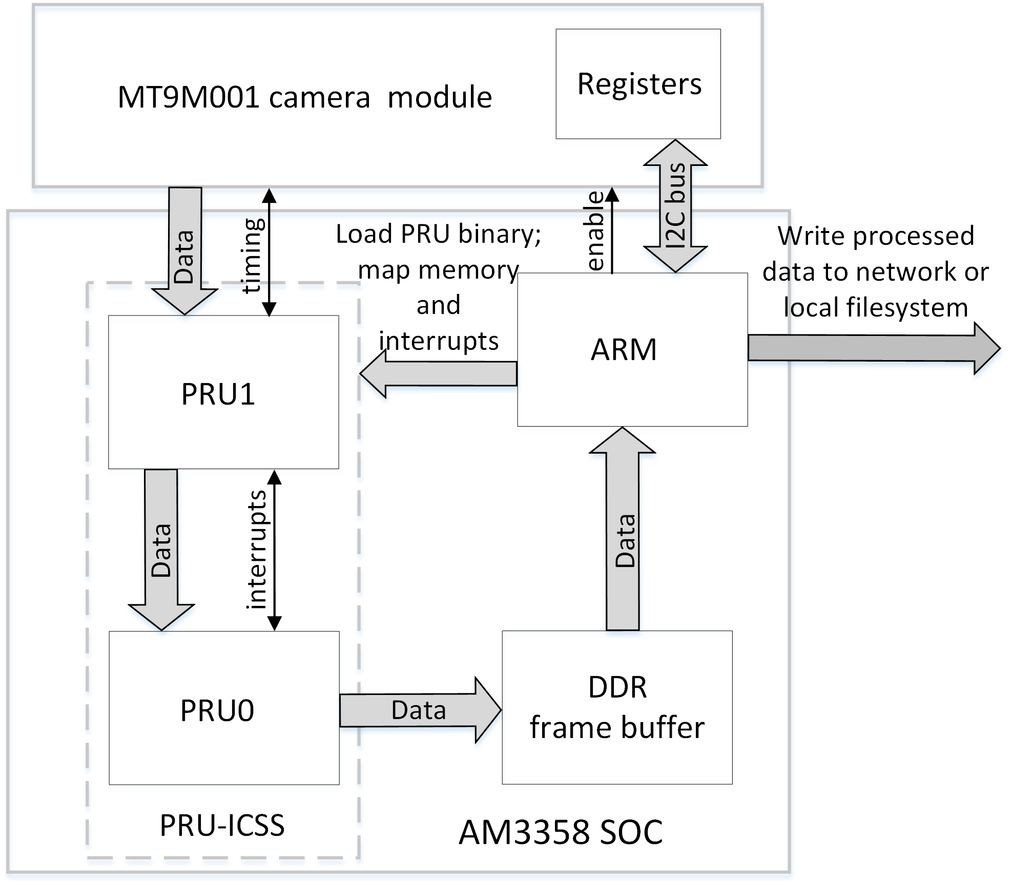
\includegraphics{cmos1/image1.png}
\end{figure}

\begin{figure}[h] \label{cm1image2}
\caption{ (a) An image of the camera,
and (b) the camera's quantum efficiency in single-photon counting mode
as a function of x-ray photon energy, as established by comparison with
a commercial Si drift detector. The glass cover of the CMOS sensor has
been removed to allow direct x-ray detection.}
\centering
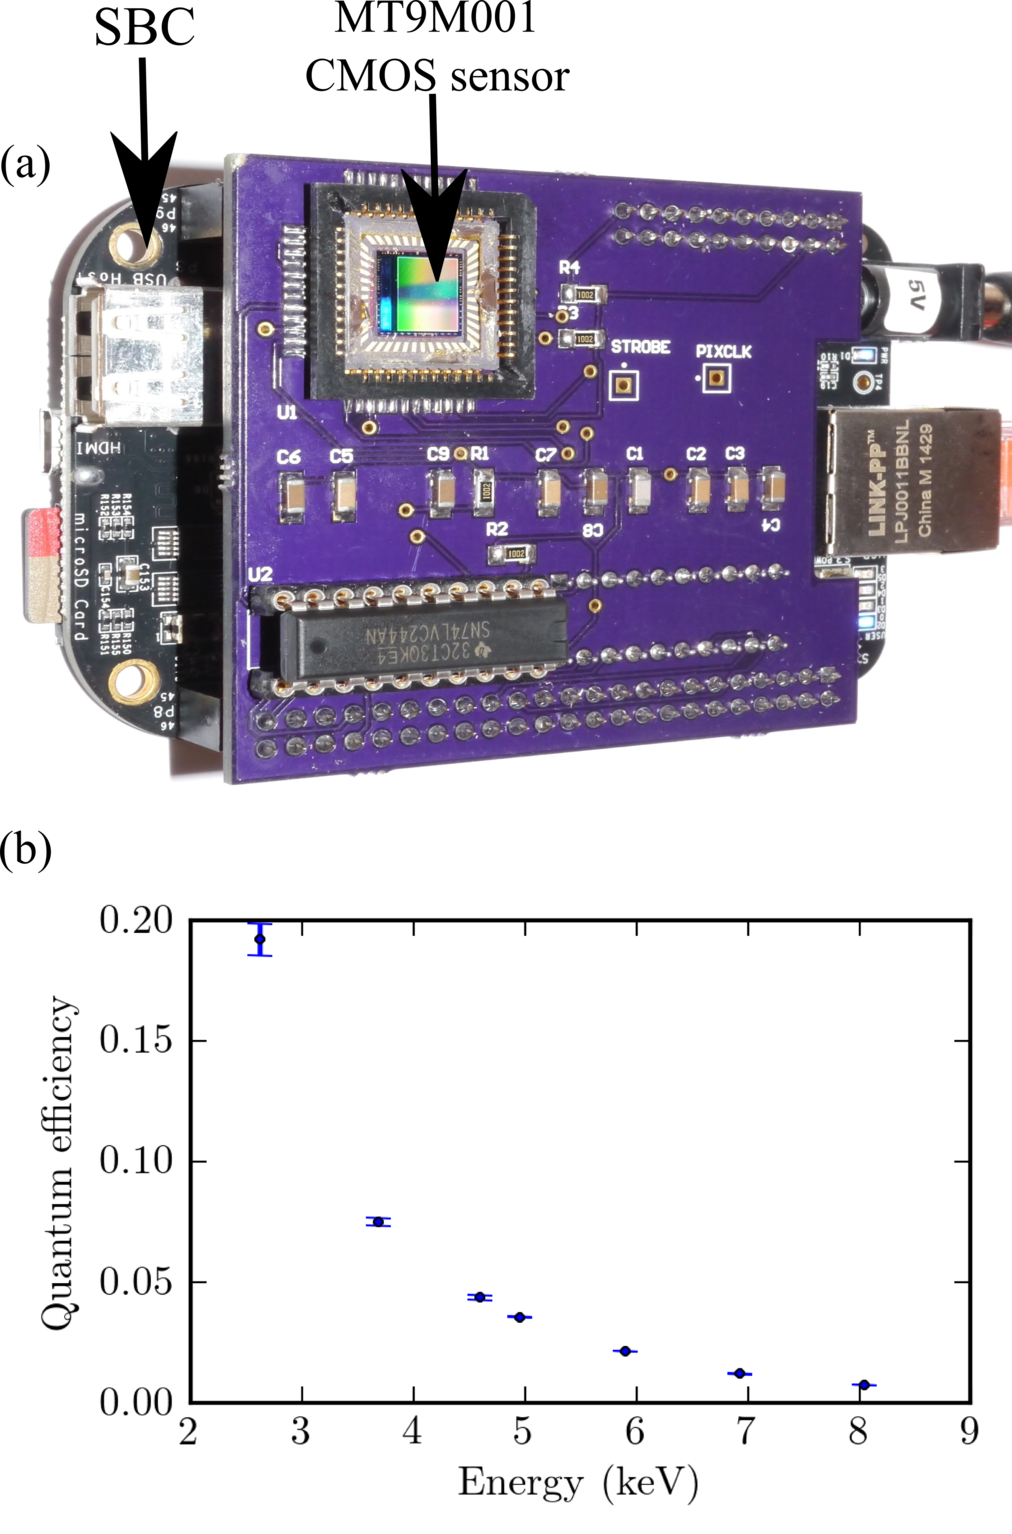
\includegraphics{cmos1/image2.png}
\end{figure}

\FloatBarrier

Multiple steps in processing are all performed on the SBC, and processed
data is stored on the SBC's SD card before transfer to the control
workstation. An exposure sequence accumulates the sum of all individual
frames as a single image. Additionally, a spectrum is generated by
binning the number of pixels per ADC channel. The finest energy
resolution requires operating the sensor in the low-intensity single
photon counting (SPC) regime where the mean period between photons
incident on a given pixel is significantly larger than the frame time.
Only x-ray events for which the entire charge cloud is concentrated in a
single pixel are incorporated into the spectrum; this filtering step,
which we refer to as cluster rejection, is well-established as necessary
for optimal performance in pixel detectors used for SPC
spectroscopy {[}13,19{]}\textsuperscript{,}

In cluster-rejection mode the sensor's saturation rate is 100,000
photons per second, but this can improved $\sim$3-fold by
resolving the aforementioned memory bottleneck. The quantum efficiency
(QE) of the detector was characterized by measurement of the
\emph{K}-shell fluorescence spectra of chlorine, calcium, and several
transition metals. This was done using a low-power laboratory x-ray tube
source to excite 1\emph{s} core holes of these elements in various solid
samples. The intensity of resulting
\hyperdef{}{OLEux5fLINK2}{}{\hyperdef{}{OLEux5fLINK3}{}{\hyperdef{}{OLEux5fLINK4}{}{\hyperdef{}{OLEux5fLINK15}{}{\hyperdef{}{OLEux5fLINK16}{}{\hyperdef{}{OLEux5fLINK17}{}{\hyperdef{}{OLEux5fLINK20}{}{\hyperdef{}{OLEux5fLINK21}{}{\hyperdef{}{OLEux5fLINK22}{}{\hyperdef{}{OLEux5fLINK23}{}{\hyperdef{}{OLEux5fLINK24}{}{\hyperdef{}{OLEux5fLINK25}{}{\hyperdef{}{OLEux5fLINK26}{}{\hyperdef{}{OLEux5fLINK27}{}{\hyperdef{}{OLEux5fLINK28}{}{\hyperdef{}{OLEux5fLINK29}{}{}}}}}}}}}}}}}}}}\(K_{\alpha}\)
and
\hyperdef{}{OLEux5fLINK30}{}{\hyperdef{}{OLEux5fLINK31}{}{\hyperdef{}{OLEux5fLINK32}{}{\hyperdef{}{OLEux5fLINK33}{}{}}}}\(K_{\beta}\)
emission registered by the detector was referenced to that recorded at
the same position by a commercial Si drift detector (Amptek XR-100SDD)
having known QE; results are presented in Fig. 2. Due to the small
active layer thickness of the CMOS sensor, its quantum efficiency
rapidly decreases from 19\% at 2.6 keV (Cl \(K_{\alpha}\) emission) to
$\sim$1\% at 8.0 keV (Cu \(K_{\alpha}\) emission). For
imaging applications, such as use as a position-sensitive detector in
wavelength-dispersive spectroscopy, it is clear that higher QE can be
obtained by cluster identification, i.e., including information from
events with some multipixel character. Our initial experience suggests a
50\% increase in detected photon rate, but this requires further
investigation. We expect that the QE will decrease below the Si
\emph{K}-edge because of the sudden increase in penetration length
compared to the active layer thickness, but that some utility will
remain below 1.5 keV. The present camera design is being modified for
easier vacuum compatibility and the above issue will be investigated.

We now present detector performance in two representative applications.
The radiograph in Fig. 3 (a) demonstrates the sensor's use as an imaging
detector, while Fig. 3 (b) presents a spectrum of Mn \emph{K}-shell
emission. No dark-field corrections are used here: the dark counts are
negligible in this bin range. The FWHM of the sensor's energy response
function at Mn \(K_{\alpha}\) is 280 eV, approximately two times as
large as in Fano noise-limited x-ray CCDs but still sufficiently small
for the Mn \(K_{\alpha}\) and \(K_{\beta}\) emission peaks to be
resolved. The resolution generally scales as \(\sqrt{E}\), where
\emph{E} is photon energy, for example showing 190 eV resolution at Cl
\hyperdef{}{OLEux5fLINK34}{}{\hyperdef{}{OLEux5fLINK35}{}{\hyperdef{}{OLEux5fLINK36}{}{\hyperdef{}{OLEux5fLINK37}{}{}}}}\(K_{\alpha}\)
and 330 eV at Cu \(K_{\alpha}\). The spectrum's background below the Mn
\(K_{\alpha}\) peak energy is due to incomplete collection of charge
from photon events, even after filtering for single-pixel events.

The camera's good QE below 4 keV suggests that few-keV x ray
spectroscopy, whether in direct detection or as the position sensitive
detector in a wavelength-dispersive
instrument {[}9-11{]}, would be a
particularly favorable venue. In this regime, the smaller pixel
dimension of CMOS sensors similar to the MT9M001 is a significant
advantage relative to conventional x-ray CCDs, as it enables the
combination of short working distance, high collection solid angle, and
high energy
resolution.
 {[}20-22{]} Additionally, such
CMOS sensors' much smaller (1\% or under) cost, while not in itself a
technical innovation, makes them promising candidates for disposable
direct-detection spectrometers in laser plasma experiments, for
high-resolution radiography in educational (instructional) settings, ,
and for versatile coverage of special scattering angles in synchrotron
studies.

\begin{figure}[h] \label{cm1image3}
\caption{ (a) Radiograph of a flower petal. The grayscale is a
representation of raw incident intensity. Improved spatial resolution
would be achieved by selection of single-pixel
events {[}14{]}. (b) X-ray
emission spectrum of a Mn metal foil excited by a low-power laboratory
x-ray tube source. The spectrum is based only on nominally single-pixel
events.}
\centering
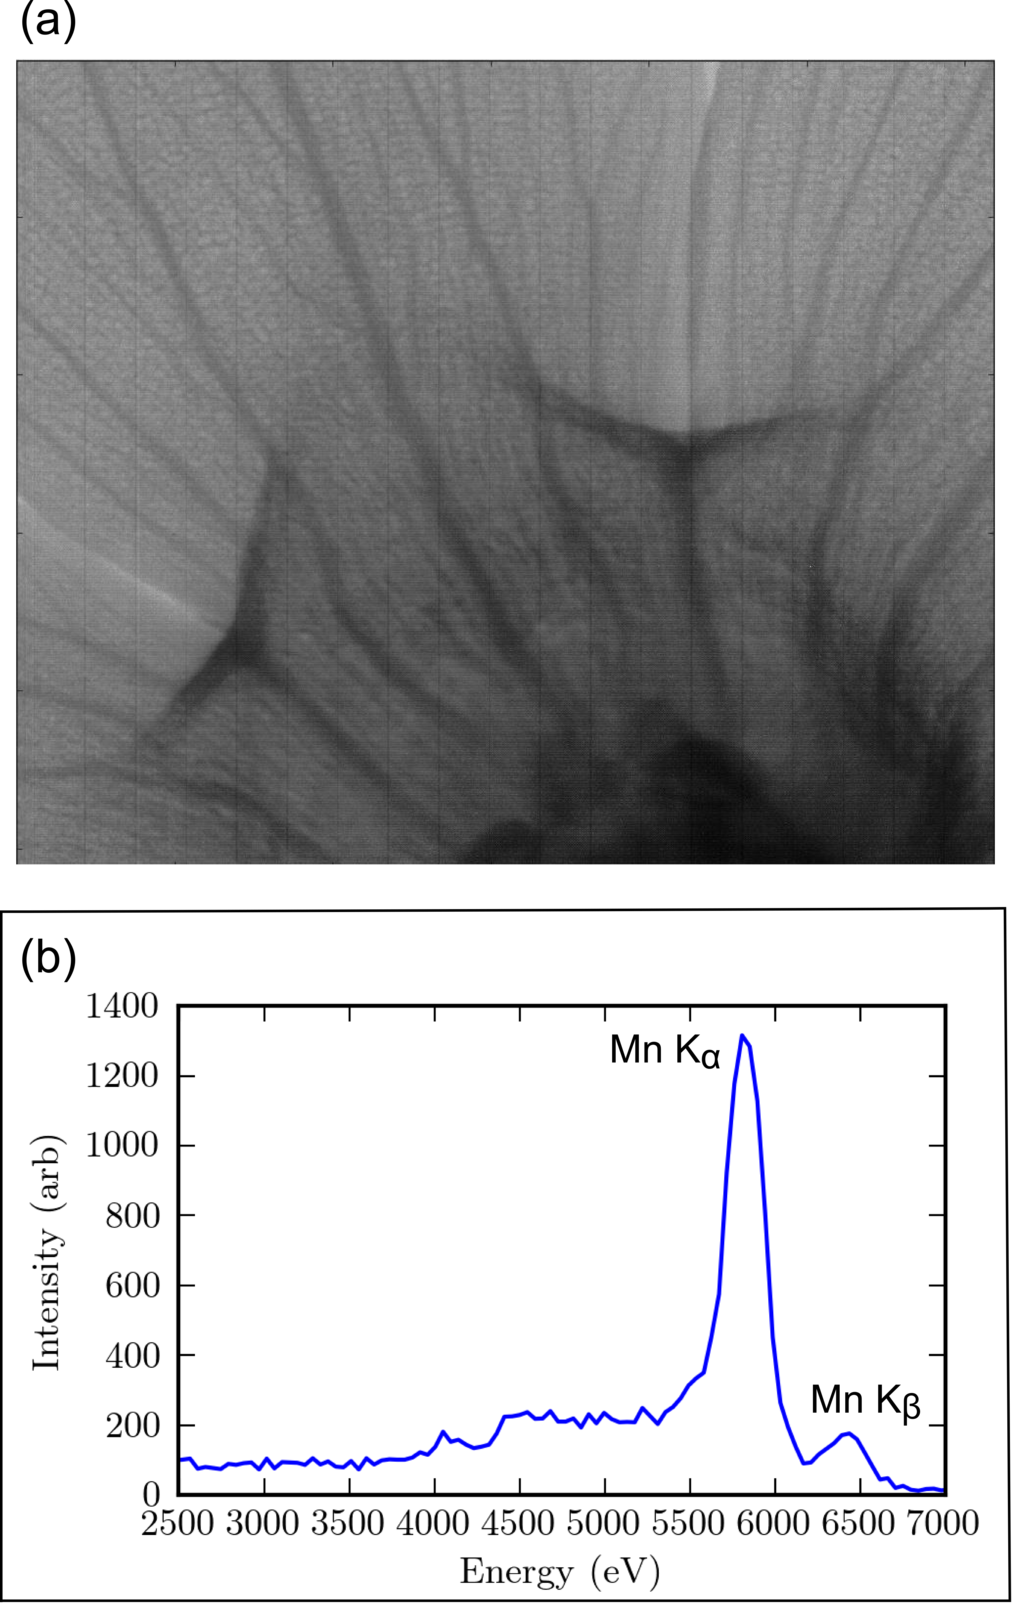
\includegraphics{cmos1/image3.png}
\end{figure}

\FloatBarrier

\section{Conclusions}
We have reported the development of a flexible and
surprisingly effective x-ray camera platform composed of standard
commercial components merged with custom electronics that can be readily
ordered from commercial prototyping services. The observed performance
suggests an interesting range of future applications at photon energies
of a few keV. This includes two aggressive possibilities: (1) large-area
spectroscopic detectors formed by multiplexing large numbers of our
cameras to reach net spectroscopic count rates useful for studies at the
highest-intensity synchrotron beamlines or at x-ray free electron
lasers, and (2) disposable detectors for use in the EMP-rich
environments of laser plasma experiments.

\section*{Acknowledgments}
This work was supported by the U.S.
Department of Energy, Basic Energy Sciences under Grant No.
DE-FG02-09ER16106 and also by the Office of Science, Fusion Energy
Sciences and the National Nuclear Security Administration thought Grant
No. DE-SC0008580. We thank Bryan Venema for assistance with board
assembly and for many useful discussions.


{[}1{]} K. Koyama, et al., Publications of the
Astronomical Society of Japan \textbf{59} (sp1), S23-S33 (2007).

{[}2{]} P. Lechner, R. Hartmann, P. Holl, G.
Lutz, N. Meidinger, R. H. Richter, H. Soltau and L. Strüder, Nuclear
Instruments and Methods in Physics Research Section A: Accelerators,
Spectrometers, Detectors and Associated Equipment \textbf{509} (1--3),
302-314 (2003).

{[}3{]} A. Stefanescu, et al., Nuclear
Instruments and Methods in Physics Research Section A: Accelerators,
Spectrometers, Detectors and Associated Equipment \textbf{624} (2),
533-539 (2010).

{[}4{]} S. R. Nagel, et al., Review of
Scientific Instruments \textbf{83} (10), 10E116 (2012).

{[}5{]} G. R. Plateau, et al., Physical Review
Letters \textbf{109} (6), 064802 (2012).

{[}6{]} E. J. Gamboa, C. M. Huntington, M. R.
Trantham, P. A. Keiter, R. P. Drake, D. S. Montgomery, J. F. Benage and
S. A. Letzring, Review of Scientific Instruments \textbf{83} (10),
10E108 (2012).

{[}7{]} I. Ordavo, et al., Nuclear Instruments
and Methods in Physics Research Section A: Accelerators, Spectrometers,
Detectors and Associated Equipment \textbf{654} (1), 250-257 (2011).

{[}8{]} M. Stampanoni, G. Borchert, P. Wyss,
R. Abela, B. Patterson, S. Hunt, D. Vermeulen and P. Rüegsegger, Nuclear
Instruments and Methods in Physics Research Section A: Accelerators,
Spectrometers, Detectors and Associated Equipment \textbf{491} (1--2),
291-301 (2002).

{[}9{]} S. Huotari, F. Albergamo, G. Vankó, R.
Verbeni and G. Monaco, Review of Scientific Instruments \textbf{77} (5),
053102 (2006).

{[}10{]} S. Huotari, G. Vanko, F. Albergamo,
C. Ponchut, H. Graafsma, C. Henriquet, R. Verbeni and G. Monaco, Journal
of Synchrotron Radiation \textbf{12} (4), 467-472 (2005).

{[}11{]} M. Kavčič, M. Budnar, A. Mühleisen,
F. Gasser, M. Žitnik, K. Bučar and R. Bohinc, Review of Scientific
Instruments \textbf{83} (3), 033113 (2012).

{[}12{]} J. Hoszowska, J. C. Dousse, J. Kern
and C. Rhême, Nuclear Instruments and Methods in Physics Research
Section A: Accelerators, Spectrometers, Detectors and Associated
Equipment \textbf{376} (1), 129-138 (1996).

{[}13{]} L. Servoli, D. Biagetti, D. Passeri
and E. S. Gattuso, Journal of Instrumentation \textbf{5} (07), P07003
(2010).

{[}14{]} F. Nachtrab, T. Hofmann, M.
Firsching, N. Uhlmann and R. Hanke, Nuclear Science Symposium Conference
Record (NSS/MIC), 2009 IEEE, pp. 1636-1639.

{[}15{]} D. W. Lane, Nuclear Instruments and
Methods in Physics Research Section B: Beam Interactions with Materials
and Atoms \textbf{284}, 29-32 (2012).

{[}16{]} K. Abe, et al., Nuclear Instruments
and Methods in Physics Research Section A: Accelerators, Spectrometers,
Detectors and Associated Equipment \textbf{400} (2), 287-343 (1997).

{[}17{]} A. D. Falcone, D. N. Burrows, Y.
Bai, M. Farris, R. Cook and S. Bongiorno, Optical Engineering and
Applications \textbf{6686}, pp. 668602-668606.

{[}18{]} G. Seidler, D. Mortensen, A.
Remesnik, J. Pacold, N. Ball, N. Barry, M. Styczinski and O. Hoidn,
Review of Scientific Instruments \textbf{85} (11), 113906 (2014).

{[}19{]} B. R. Maddox, H. S. Park, B. A.
Remington and M. McKernan, Review of Scientific Instruments \textbf{79}
(10), 10E924 (2008).

{[}20{]} J. I. Pacold, et al., Journal of
Synchrotron Radiation \textbf{19} (2), 245-251 (2012).

{[}21{]} B. A. Mattern, G. T. Seidler, M.
Haave, J. I. Pacold, R. A. Gordon, J. Planillo, J. Quintana and B.
Rusthoven, Review of Scientific Instruments \textbf{83} (2), 023901
(2012).

{[}22{]} B. Dickinson, G. T. Seidler, Z. W.
Webb, J. A. Bradley, K. P. Nagle, S. M. Heald, R. A. Gordon and I. M.
Chou, Review of Scientific Instruments \textbf{79} (12), 123112 (2008).


../pandoc/cmos2.tex

\chapter{Real-time analysis tools for the LCLS}
\label{xap}

A significant drawback of current XFELs, compared to synchrotron light sources, is that they are capable of providing photons to only one endstation at a time. As a result they are vastly oversubscribed, and beamtime is granted in small allocations through highly competitive selection processes. Experimental teams therefore have strong incentives to make the most efficient possible use of beam time. Focusing on the specific case of the LCLS, the high power of the XFEL source (and its 120 Hz repetition rate) facilitates rapid completion of experiments by making very high data collection rates possible . However, fully taking advantage of high data throughput is a problem unto itself, as experiments cannot be fully scripted in advance; it is in practice necessary to make rapid evaluations based on measurement of beam conditions (which, in two-color mode, can be strongly variable), the statistical quality of incoming data, and tentative physical interpretations in the incoming data. This feedback often guides important decisions, such as beam tuning and the motion of samples and detectors. 

With the goal of addressing this problem we have developed a software package for real-time analysis and visualization of data in XFEL experiments at the LCLS. The software is implemented using Photon Science Analysis (psana), the internal data analysis framework at the LCLS, and can be run in distributed fashion over hundreds of cores. \ref{damiani2016linac} It attempts to enable a more effective analysis workflow than currently available to LCLS users, excluding those doing specialized experiments of well-established types for which there already exist tailored software packages (such as Cheetah for serial femtosecond crystallography). \ref{barty2014cheetah}

This chapter describes a Python API that that provides high-level analysis and visualization functions that directly implement common analysis operations, and can serve as building blocks more complex custom ones. The API is optimized for use through the Jupyter notebook, and it leverages the rich interactive plotting features available in that environment.

Though it will not be discussed in detail, we note the existence of a second interface to the same analysis framework, consisting of a web application that provides a more user-friendly graphical interface (in exchange for reduced flexibility). This interface was independently developed by Ryan Valenza from the Seidler group.



\section{Integration of Logging and Analysis}
The psana API associates every LCLS pulse (referred to as an event) with two integers, a run number and event number. \ref{damiani2016linac} A run contains a consecutive sequence of events; the maximum number of events in a run is determined by a 17 bit 360 Hz `fiducial' counter that the LCLS timing system distributes to each detector. The association of run/event number combinations to LCLS pulses is in practice further constrained by endstation-specific software and instrumental details: at the Matter of Extreme Conditions beamline (MEC), for example, performing a two-dimensional sample raster involves interruptions between horizontal rows, which in turn requires the run number to be incremented at the beginning of each row. 

Because the LCLS DAQ system does not allow the association of events with user-provided metadata, LCLS users must maintain separate experimental logs in which, for each run number and range of event numbers, they record information related to sample type, beam conditions, and other relevant experimental parameters.  In the vast majority of cases, users' analysis scripts directly expose psana's data access API, requiring them to explicitly specify datasets in terms of lists of run numbers. To do this the user must manually look up and transcribe information from the experimental logbook, an operation that becomes time-consuming (and potentially error-prone) when frequently repeated, as it usually must be.

% TODO: words
\begin{figure}[h] \label{uwxap_block}
\caption{Diagram summarizing the analysis software's architecture.}
\centering
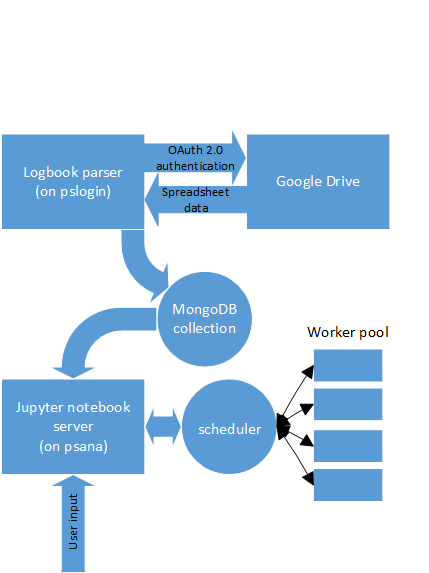
\includegraphics[scale=0.90]{../Figures/UWXAP_block_diagram.png}
\end{figure}

In response, we've made a step to unify the workflows for experimental logging and analysis. We've defined a simple query language with which the user can construct datasets defined by matches to metadata attributes recorded in the experimental logbook. The implementation is described in Fig. \ref{uwxap_block}; briefly, it consists of a daemon (i.e. application component) that accesses data from standard-formatted Google Drive spreadsheets tied to users' personal Google accounts. This daemon parses spreadsheet data into a graph structure associating run numbers with metadata column values and constructs datasets (i.e., sets of run numbers) by parsing user-provided queries on those column values. 

\section{Interactive Distributed Computing}
A second feature of the software is the simplified fashion in which it leverages the LCLS computing cluster. To do real-time analysis during beam runs it is typically necessary to scale one's workload over tensor hundreds of CPU cores. This is typically done with a batch processing workflow, where command lines for launching parallel analysis scripts are submitted to the LCLS's Platform Load Sharing Facility (LSF), which schedules them for execution on nodes of the cluster. Once a batch job is complete, users typically run a second (non-distributed) program to load and visualize the output data. The time that elapses between submission of a batch job and when it begins running is typically on the order 10 seconds or more, assuming an empty job queue. The separation between the steps of submitting an analysis batch job and loading and viewing its results introduces a delay as well, because the user must manually intervene at two points in the analysis pipeline. These two factors give a batch-processing-based workflow significant overhead. 

Our software package offers a significant improvement in this respect: the backend of the analysis API distributes calculations over the LCLS cluster transparently, with no need for the user to submit batch jobs or otherwise steer the parallel computation in any way. Distributed computation is implemented using the parallel computing utility pathos, which allows scatter-gather style computation using the same API as Python's multiprocessing module, but with more flexible serialization capability implemented by the module dill. 


\begin{figure}[h] \label{uwxap_screenshot}
\caption{Jupyter notebook screen capture demonstrating a simple example of the API's usage. First a dataset is defined via a query matching all run numbers between 200 and 210 for which the recorded value for the XFEL transmission is 0.11. Two metadata attributes of the resulting dataset are then printed. In the last line of input, we call the API function datashow.show, which takes a list of datasets (in this case containing the single defined dataset) and an area detector identifier (in this case `si', the identifier for a downstream silicon spectrometer monitoring the XFEL spectrum) and displays the average of detector readouts over all events. This data was collected at LCLS beam run LK20. }
\centering
\includegraphics[scale=0.80]{../Figures/UWXAP_si_screenshot.png}
\end{figure}

\section{API features}
The last component of our package is a library of API functions for analyzing and visualizing data. These are in part tailored to MEC, the location of both our LCLS beam runs, but are for the most part generally applicable to other endstations. The API heavily leverages features of the browser-based Jupyter notebook, including interactive Javascript-based plots.


The API provides standard analysis routines for spectroscopy and X-ray powder diffraction. Miscellaneous diagnostic tools are included for, e.g., viewing the readout of area detectors (per-event or averaged over all events in a dataset) and generating histograms or scatter plots of event-by-event signal incident on arbitrary detectors. Most of these functions adopt a general functional programming style that allows the user to alter their behavior, using them as building blocks in more complex, customized applications. For instance, all analysis API calls accept, as optional arguments, user-defined functions for event rejection that take a detector datum as input and return a boolean. A more specialized example of the functions-as-arguments pattern is the histogram API call. In its most basic usage, this function takes an area detector identifier and one or more datasets as arguments, and returns an interactive figure containing histograms of per-event integrated signal on the detector. In a more sophisticated usage, the user could pass in a keyword parameter consisting of a function that, for example, integrates signal over a subregion of the area detector's 2D data array, instead of its entirety. 

This software is under continued development. The primary ongoing effort is an overhaul of the parallel-processing backend to use the distributed computing library Dask. Dask's valuable features, in our context, include a task scheduler with the ability to dispatch work to a pool of worker processes in intelligent fashion (with awareness of task dependencies and data locality), and with flexibility and fault tolerance--allowing, for example, the dynamic addition and removal of worker processes. 




\cleardoublepage
\printbibliography[heading=bibintoc, title={References}]


\end{document}
